A fit using data is performed on using all bins, without blinding. The signal sample is also included in the fit (it is a signal+background fit). The unblinded data fit is performed over all control and signal regions (combined 1L+2LOS), and with all available samples and systematics. The dominant \ttbar background is reweighted using the NN method.

The post-fit distributions associated with each background and signal region are shown in Figure \ref{fig:unblinded_data_SplusB_postfit_1L} for 1L regions and Figure \ref{fig:unblinded_data_SplusB_postfit_2L} for 2LOS regions from the combined fit using mass point $m_H=400$ GeV. The nuisance parameter pulls and constraints are compared between 1L, 2LOS, and the combined fit in Figures \ref{fig:unblinded_data_SplusB_NP_instrumental}, \ref{fig:unblinded_data_SplusB_NP_ttbar}, and \ref{fig:unblinded_data_SplusB_NP_other}. Comparison for the fits using GNN outputs trained on various mass points are shown in Figures \ref{fig:unblinded_data_SplusB_NP_mass_instrumental}, \ref{fig:unblinded_data_SplusB_NP_mass_ttbar}, and \ref{fig:unblinded_data_SplusB_NP_mass_other}. Correlation matrices for systematics for the fit are shown in Figure Figure \ref{fig:unblinded_data_SplusB_corr_mH400_Data_all}.

\begin{figure}[htbp!]
        \begin{center} \setlength{\tabcolsep}{2.5pt}\footnotesize
        \begin{tabular}{cccc}
        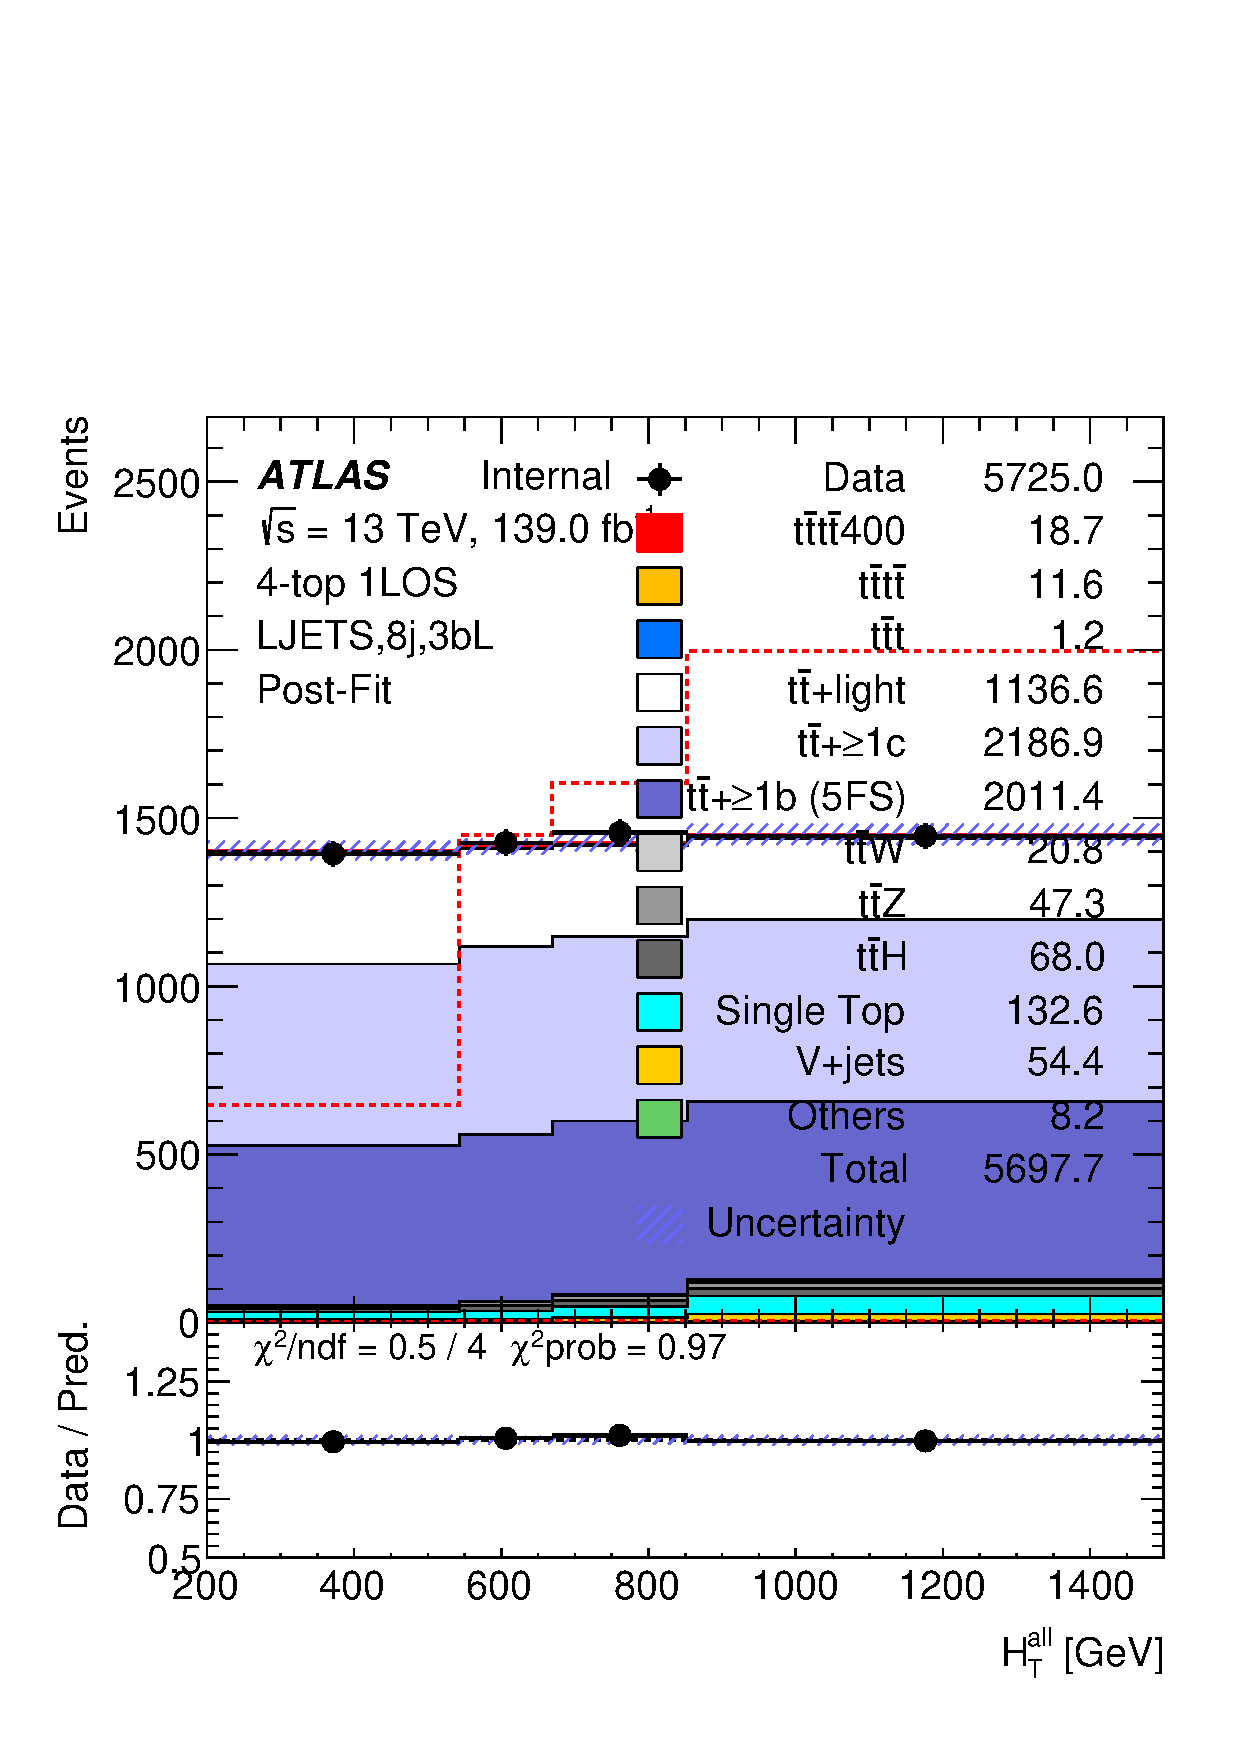
\includegraphics[width=0.23 \textwidth]{figures/fits/GNN/400/all/data_unblindedSplusB/Plots/ljets_8j3bL_postFit.pdf} &
        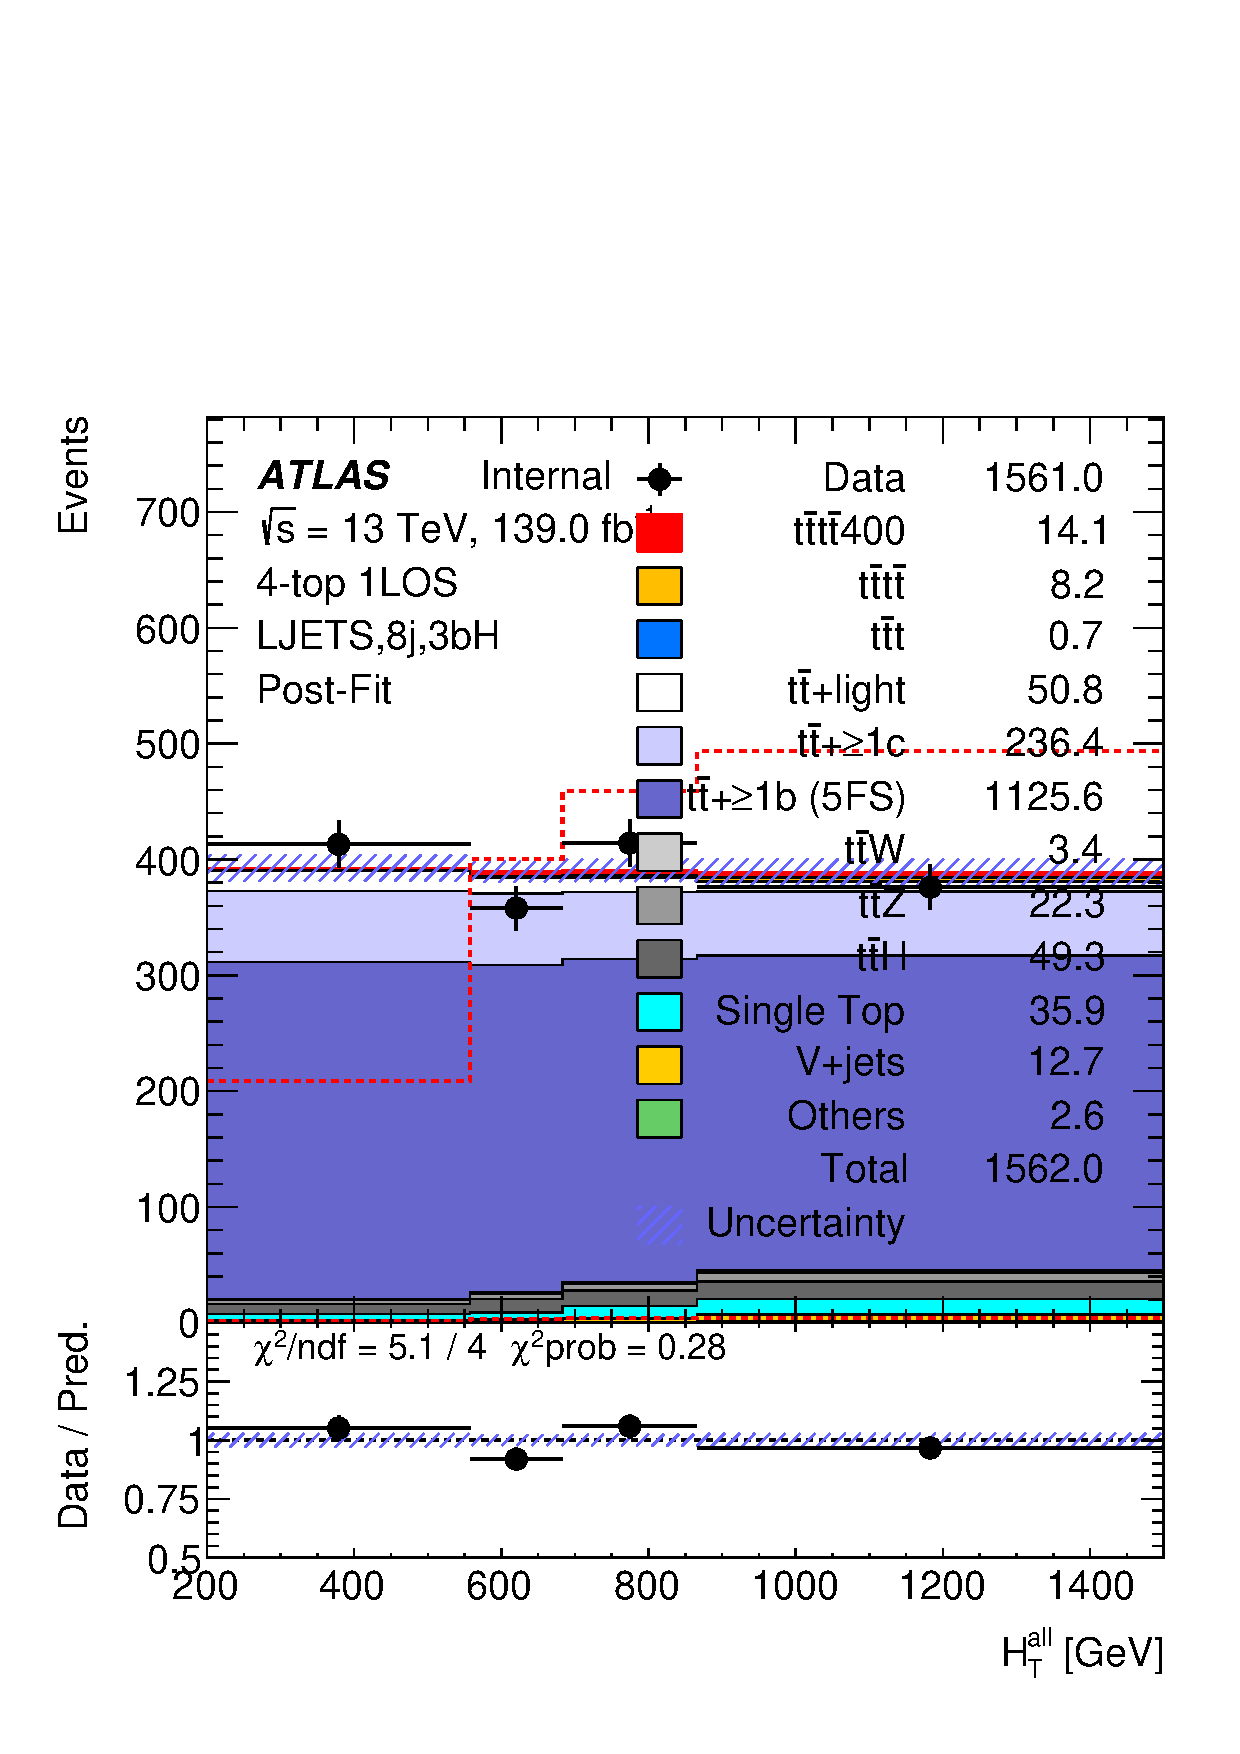
\includegraphics[width=0.23 \textwidth]{figures/fits/GNN/400/all/data_unblindedSplusB/Plots/ljets_8j3bH_postFit.pdf} &
        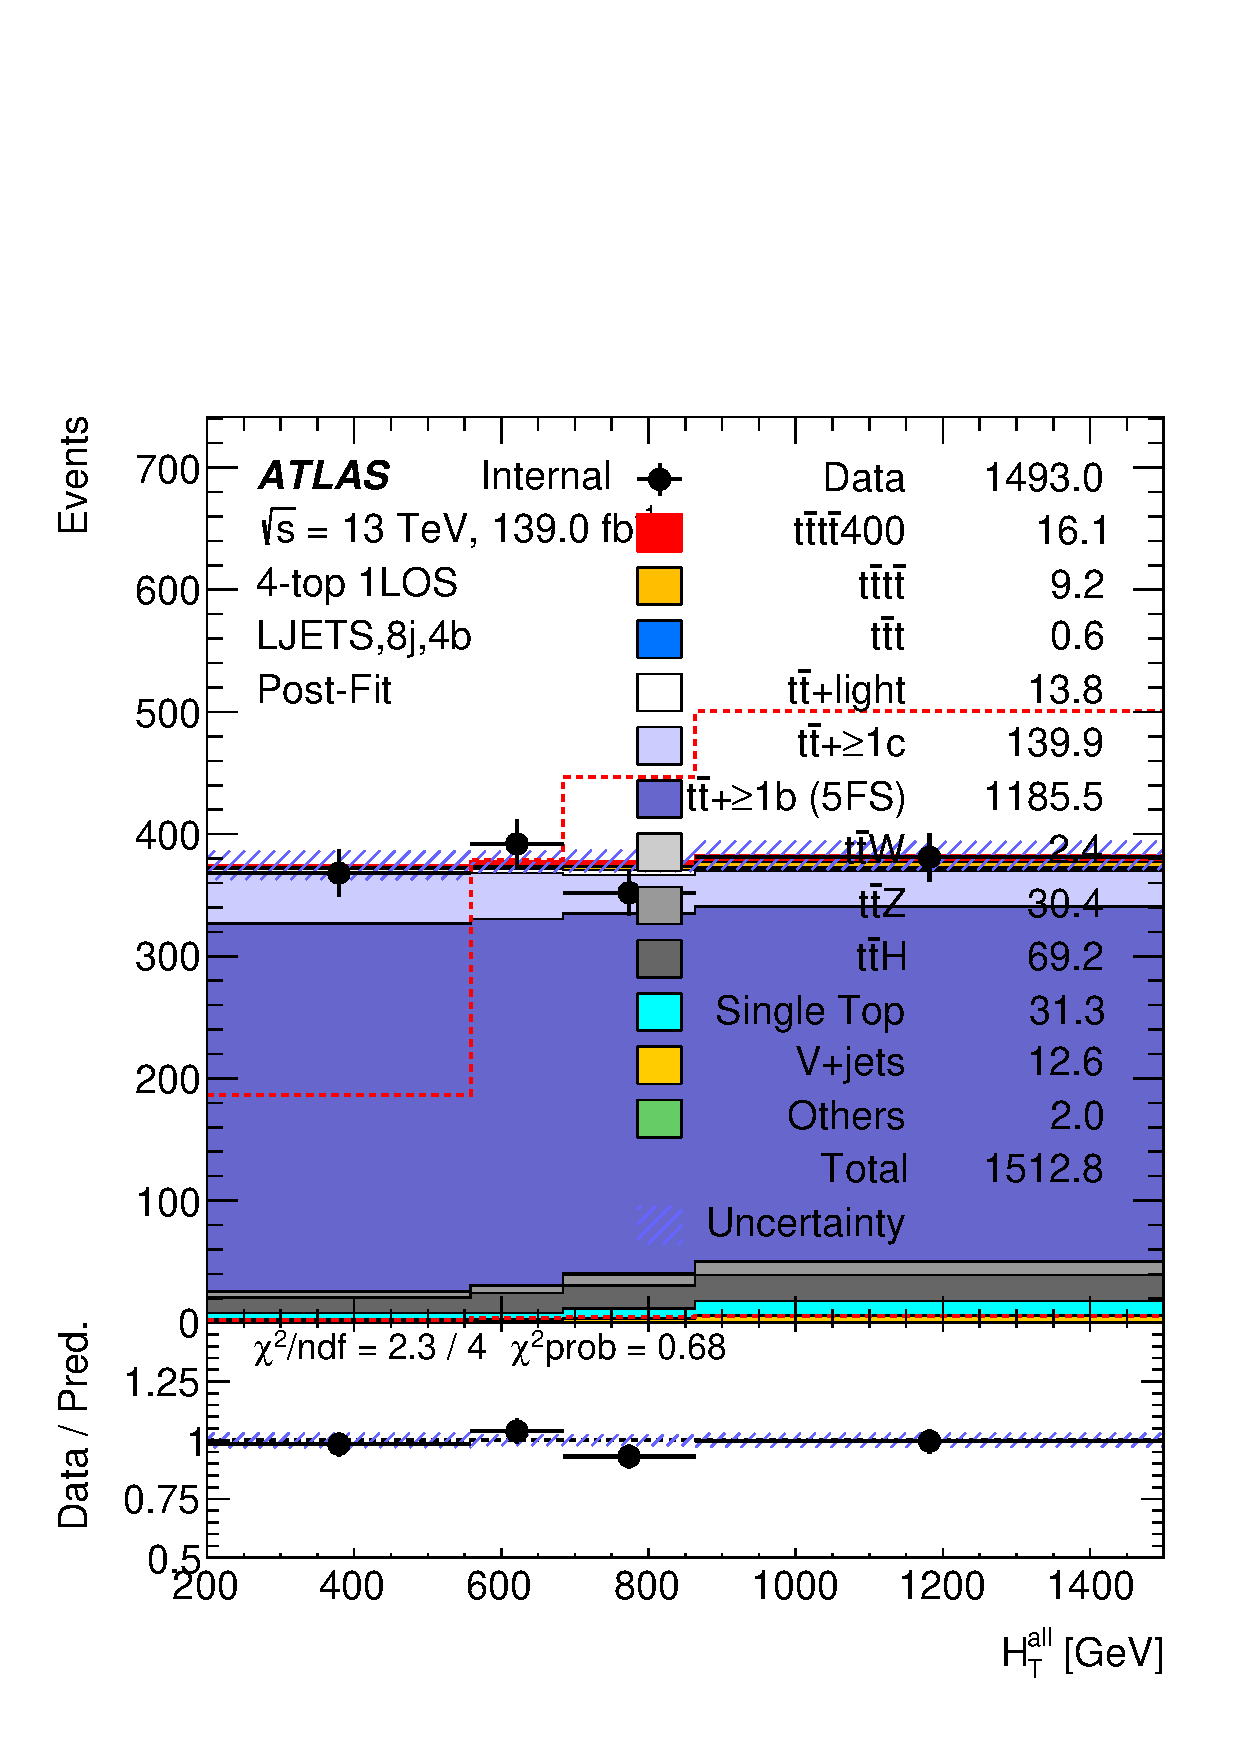
\includegraphics[width=0.23 \textwidth]{figures/fits/GNN/400/all/data_unblindedSplusB/Plots/ljets_8j4b_postFit.pdf} &
        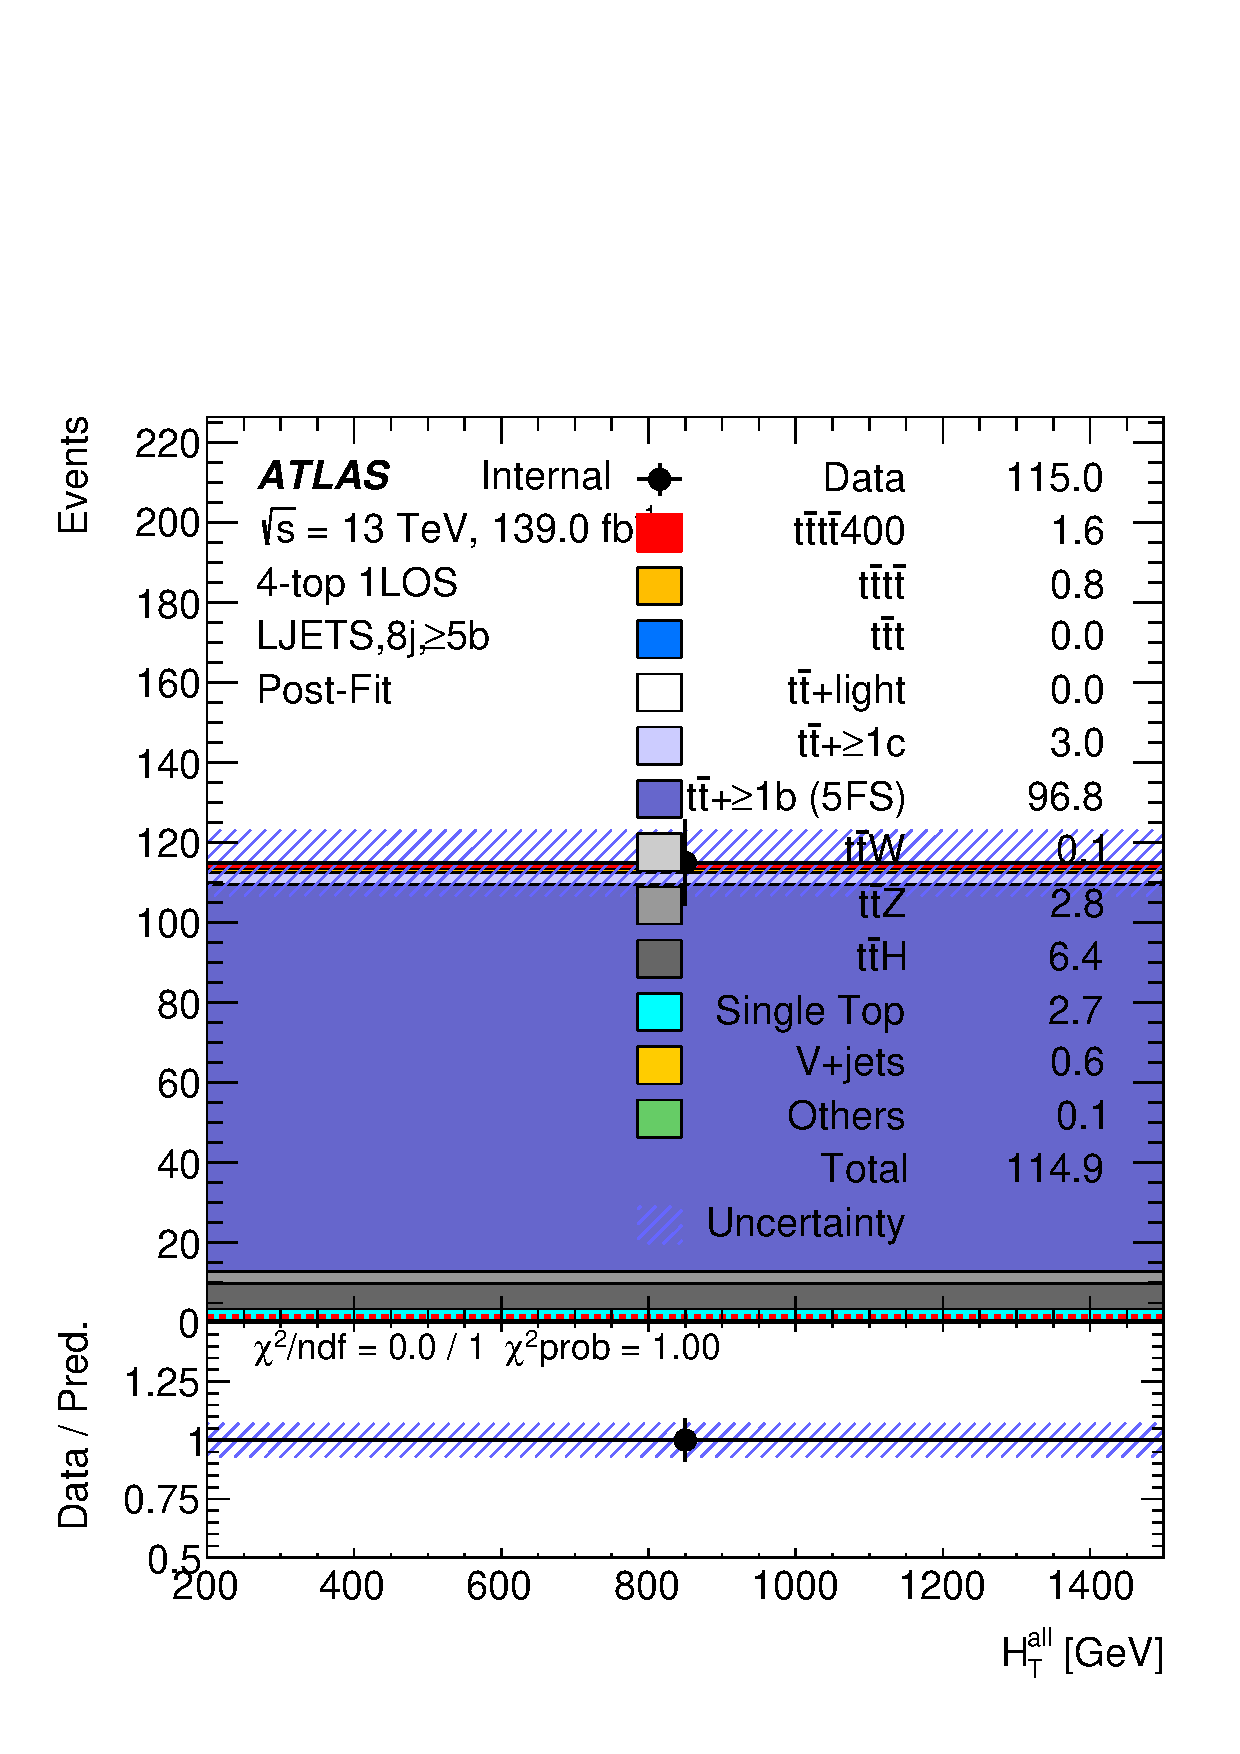
\includegraphics[width=0.23 \textwidth]{figures/fits/GNN/400/all/data_unblindedSplusB/Plots/ljets_8jge5b_postFit.pdf}\\

        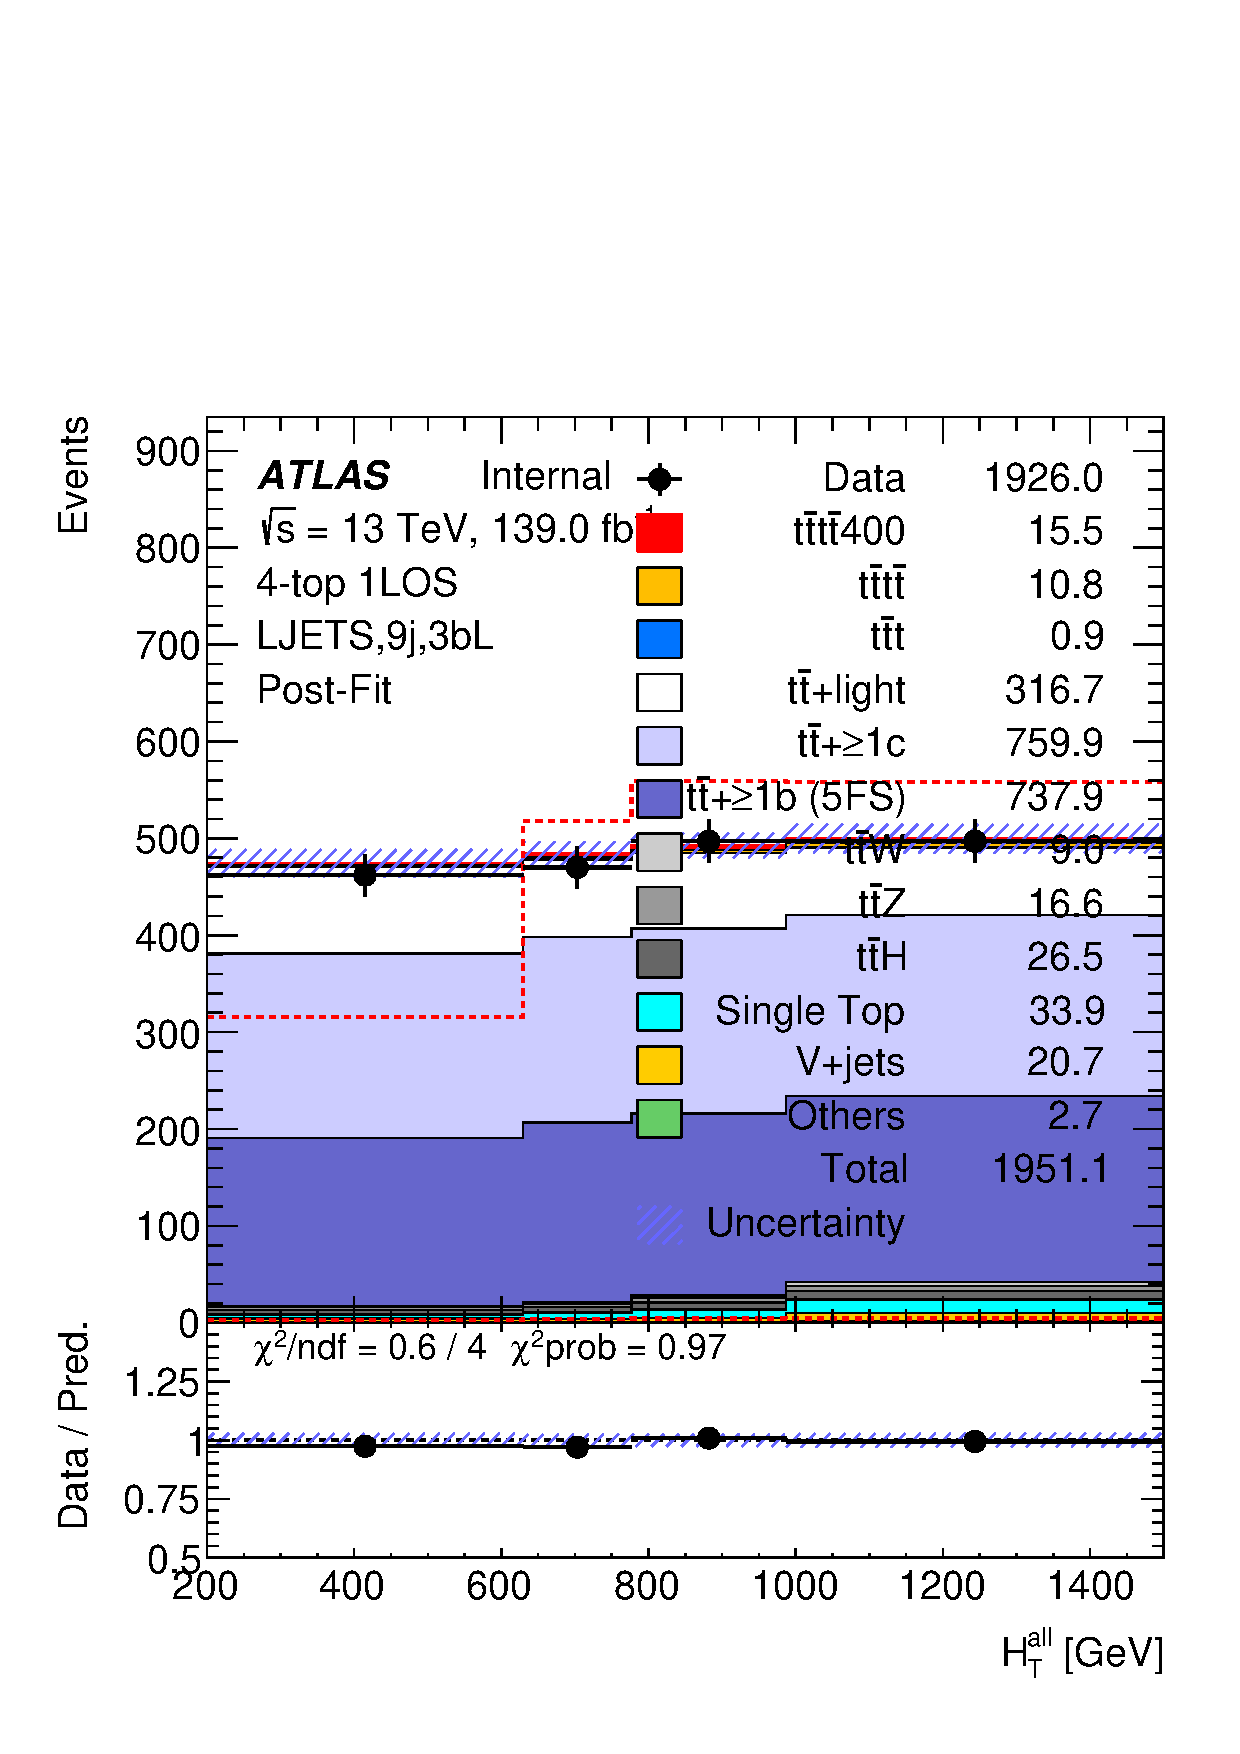
\includegraphics[width=0.23 \textwidth]{figures/fits/GNN/400/all/data_unblindedSplusB/Plots/ljets_9j3bL_postFit.pdf} &
        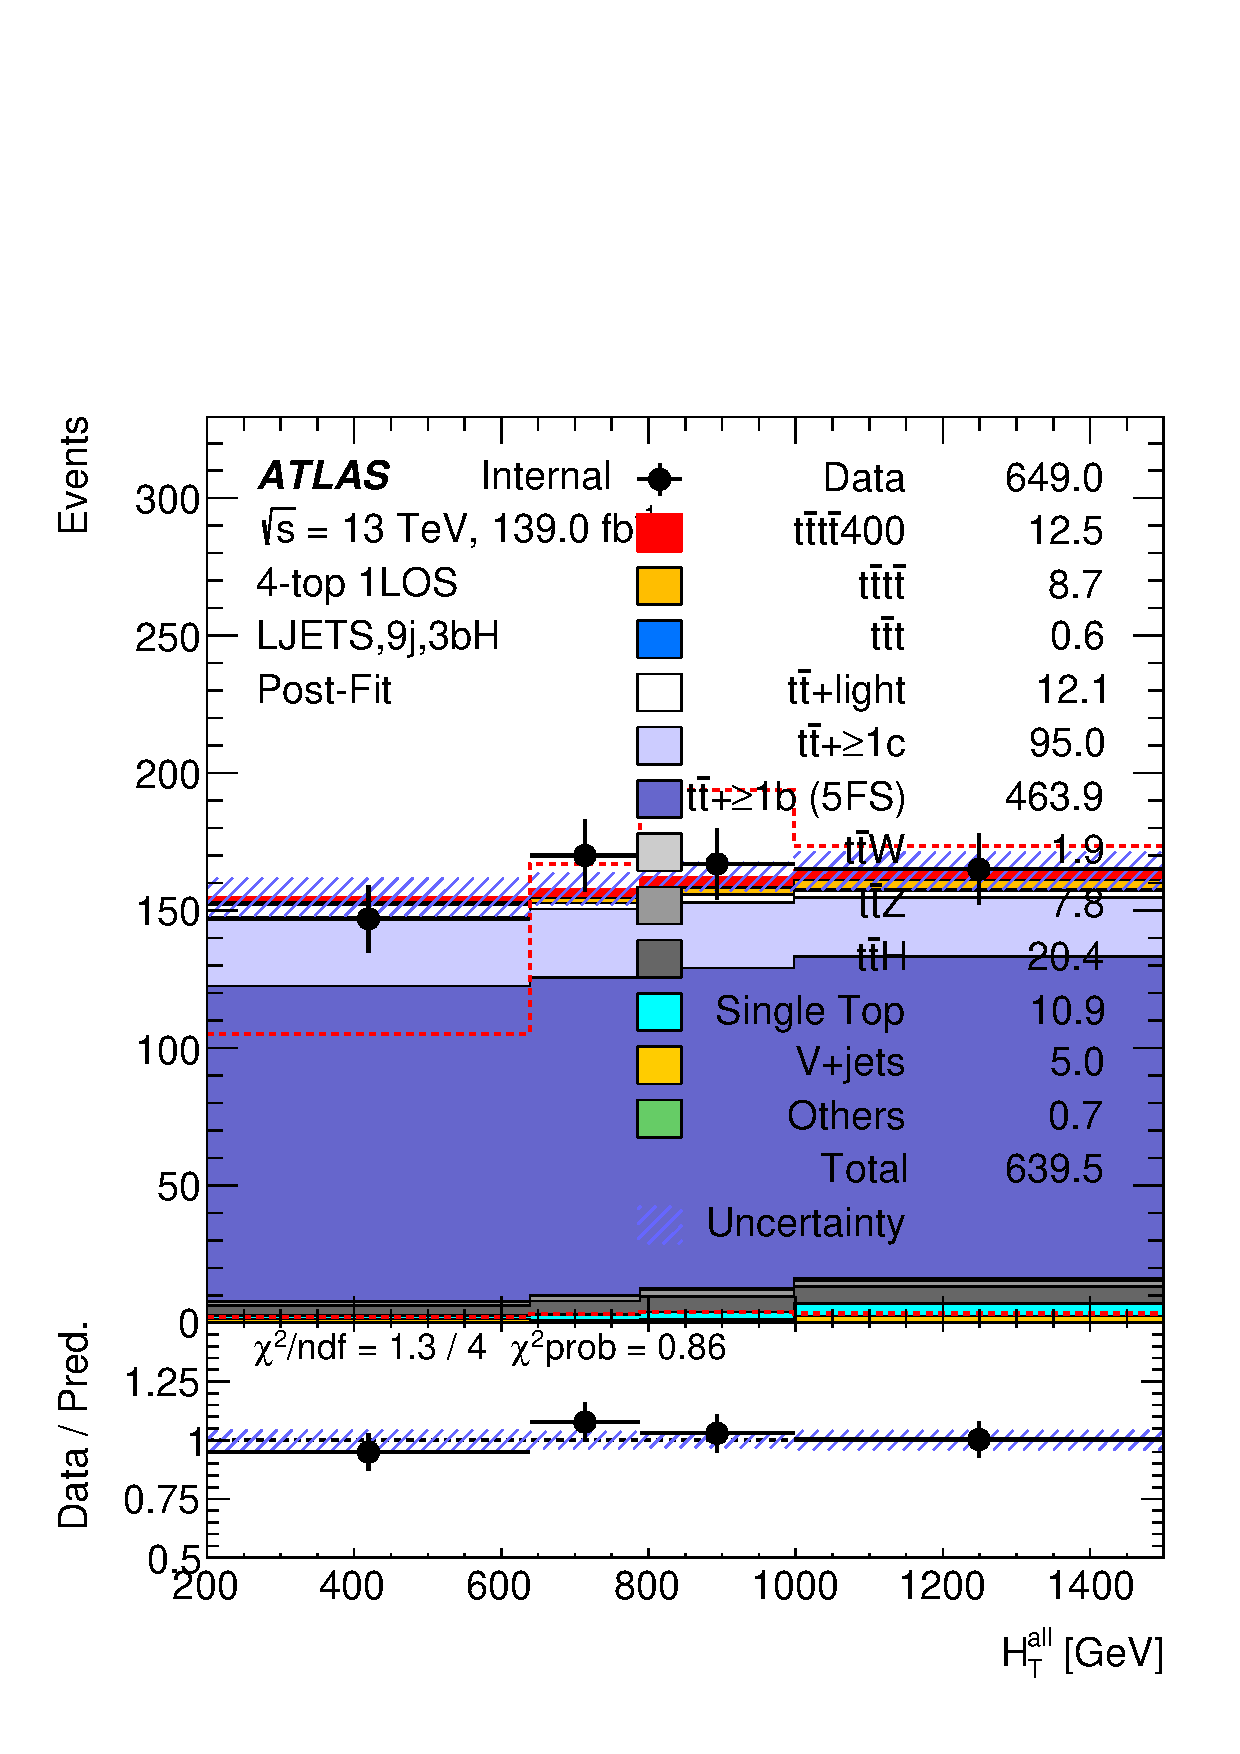
\includegraphics[width=0.23 \textwidth]{figures/fits/GNN/400/all/data_unblindedSplusB/Plots/ljets_9j3bH_postFit.pdf} &
        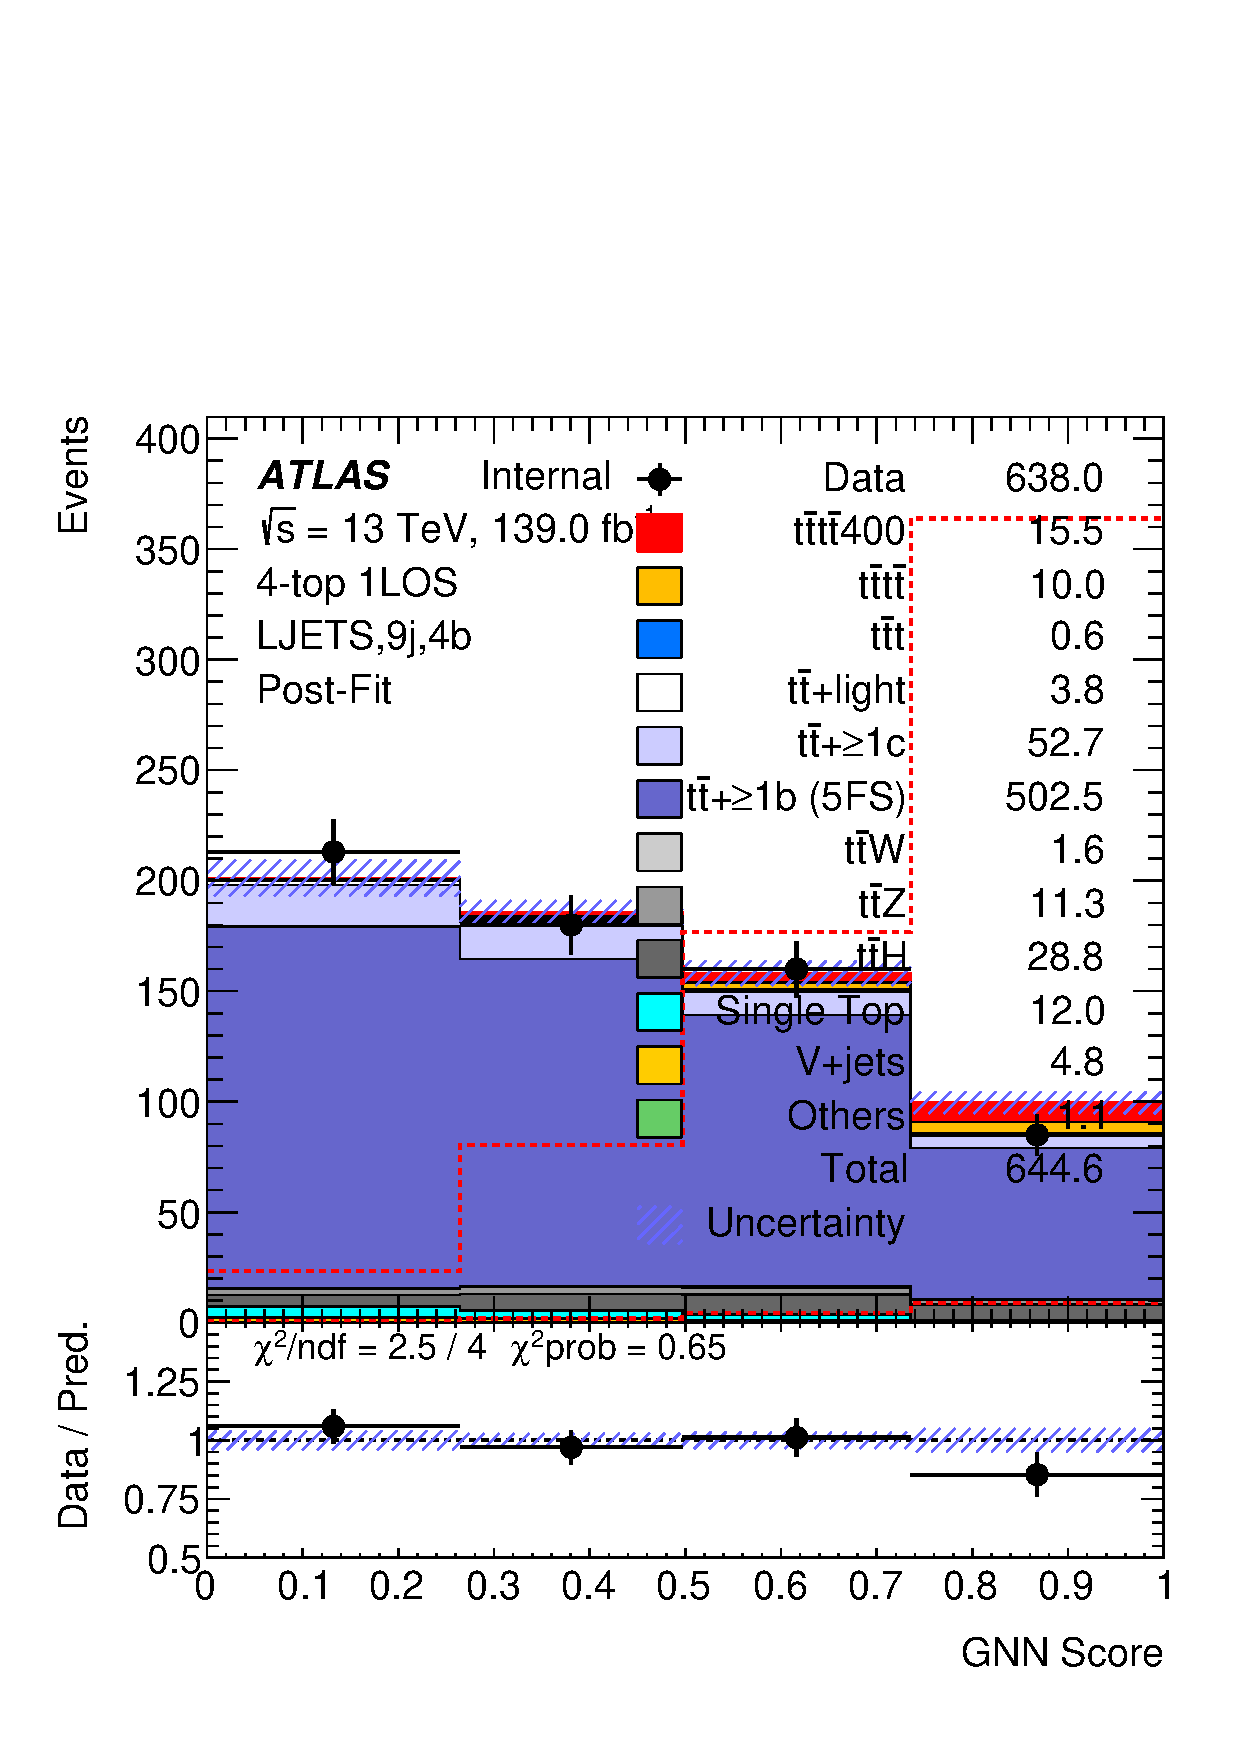
\includegraphics[width=0.23 \textwidth]{figures/fits/GNN/400/all/data_unblindedSplusB/Plots/ljets_9j4b_postFit.pdf} &
        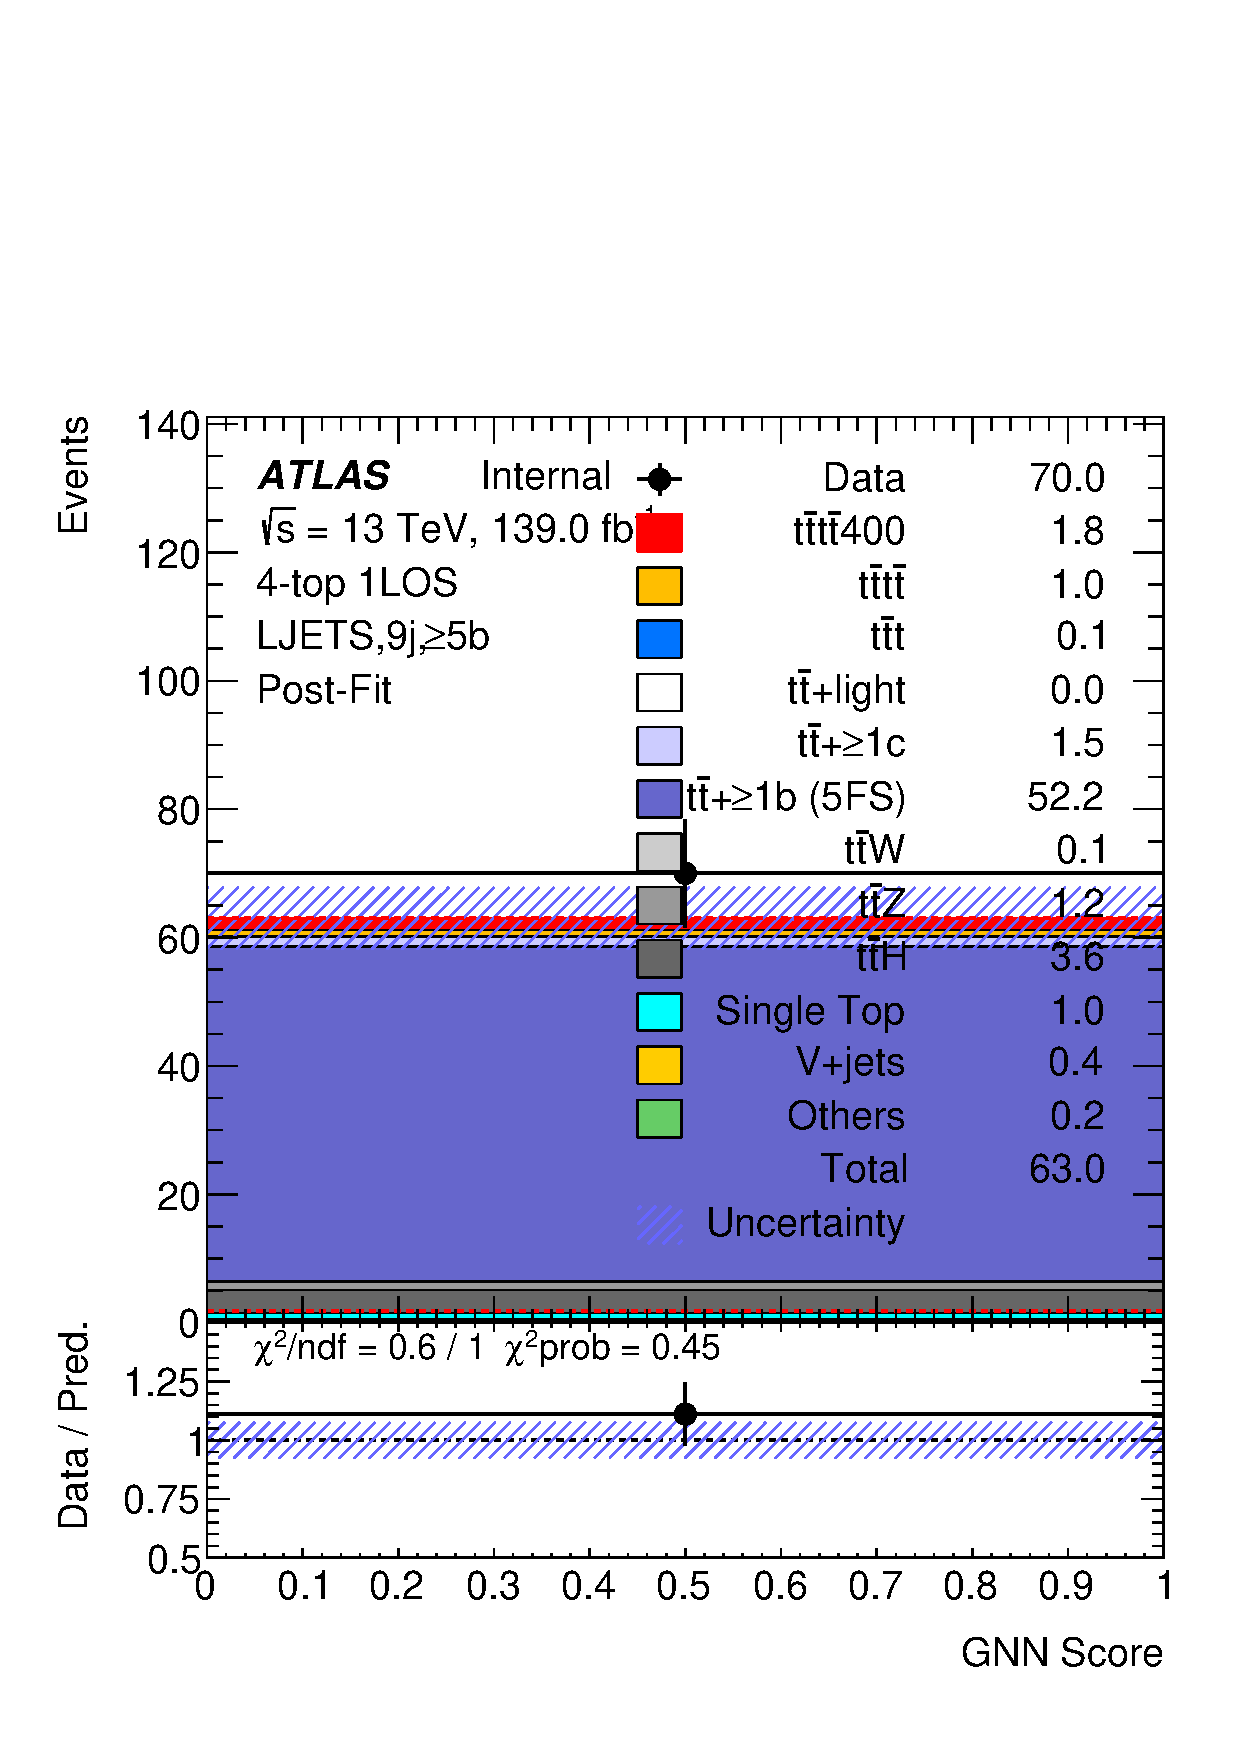
\includegraphics[width=0.23 \textwidth]{figures/fits/GNN/400/all/data_unblindedSplusB/Plots/ljets_9jge5b_postFit.pdf} \\

        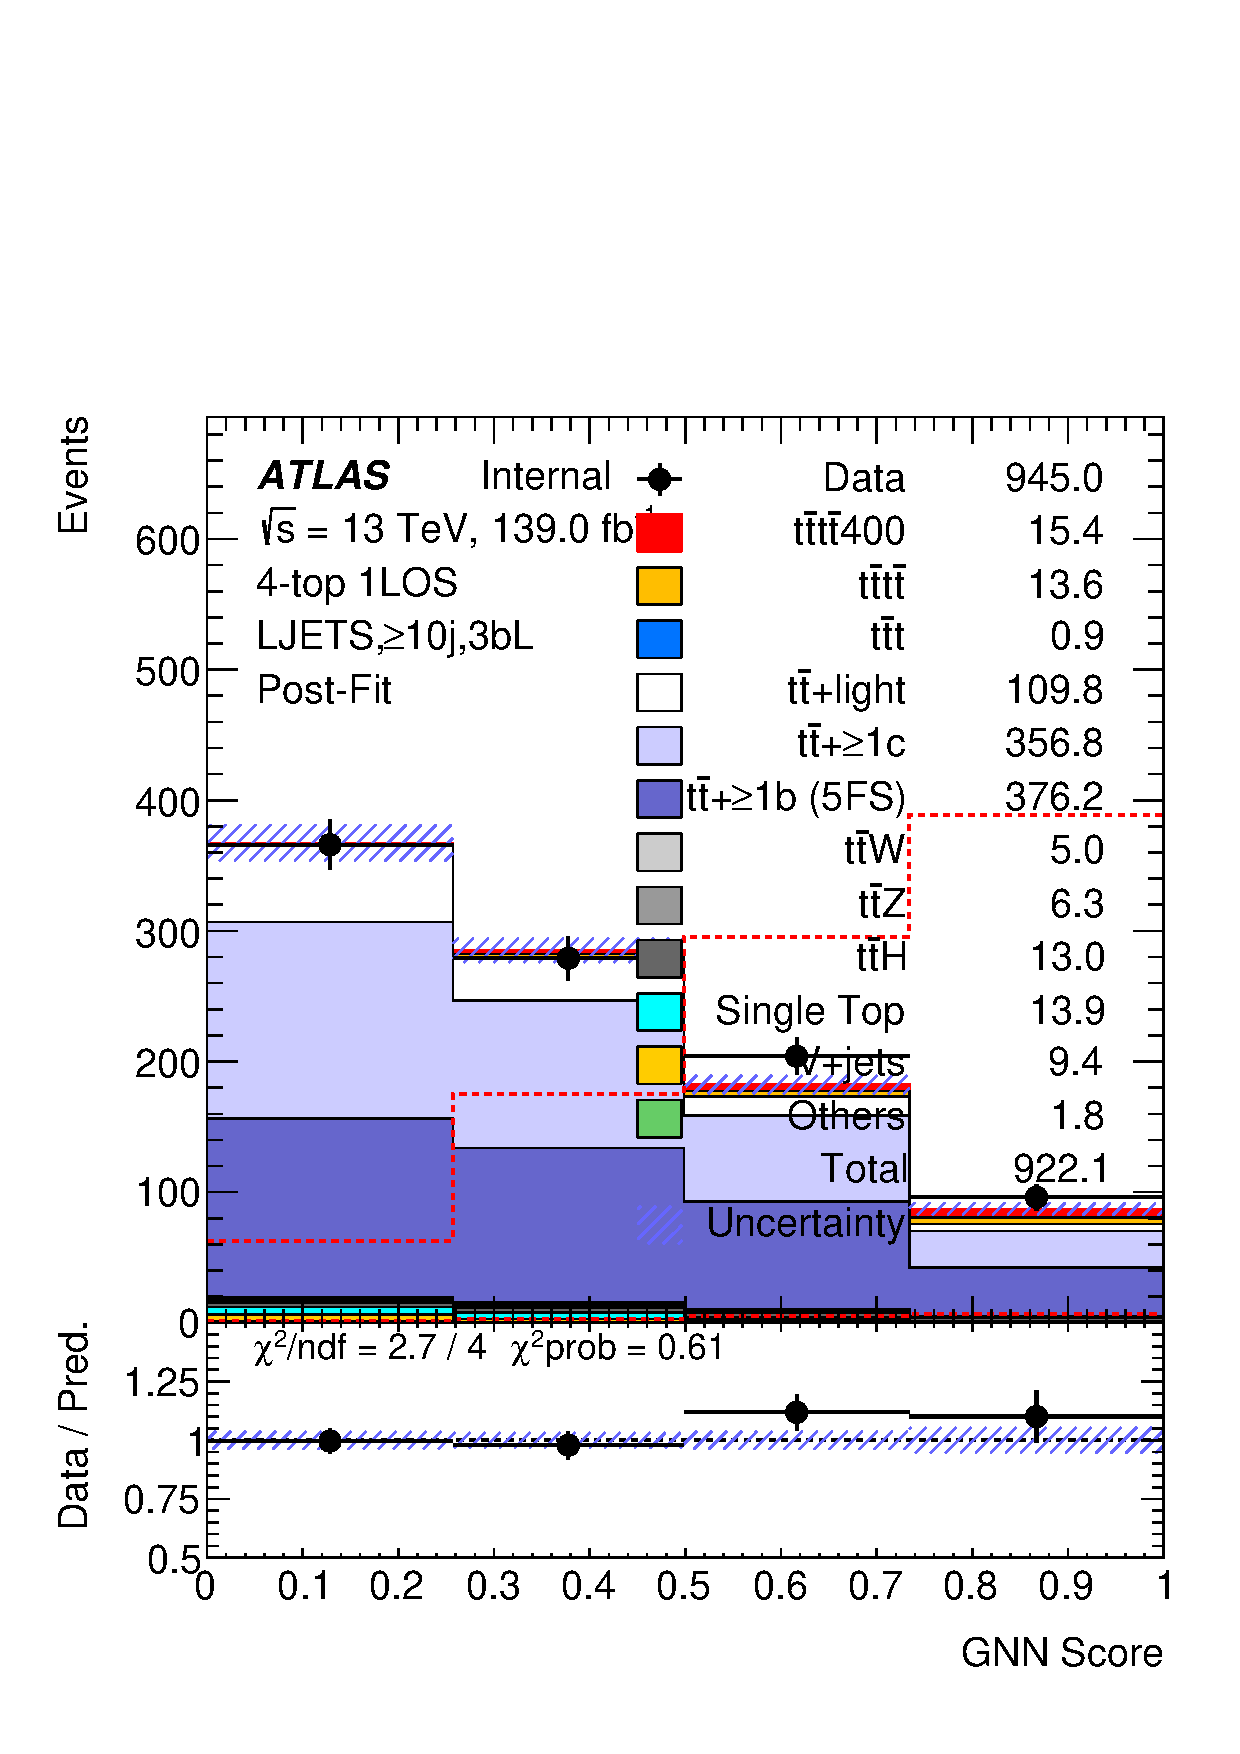
\includegraphics[width=0.23 \textwidth]{figures/fits/GNN/400/all/data_unblindedSplusB/Plots/ljets_ge10j3bL_postFit.pdf} &
        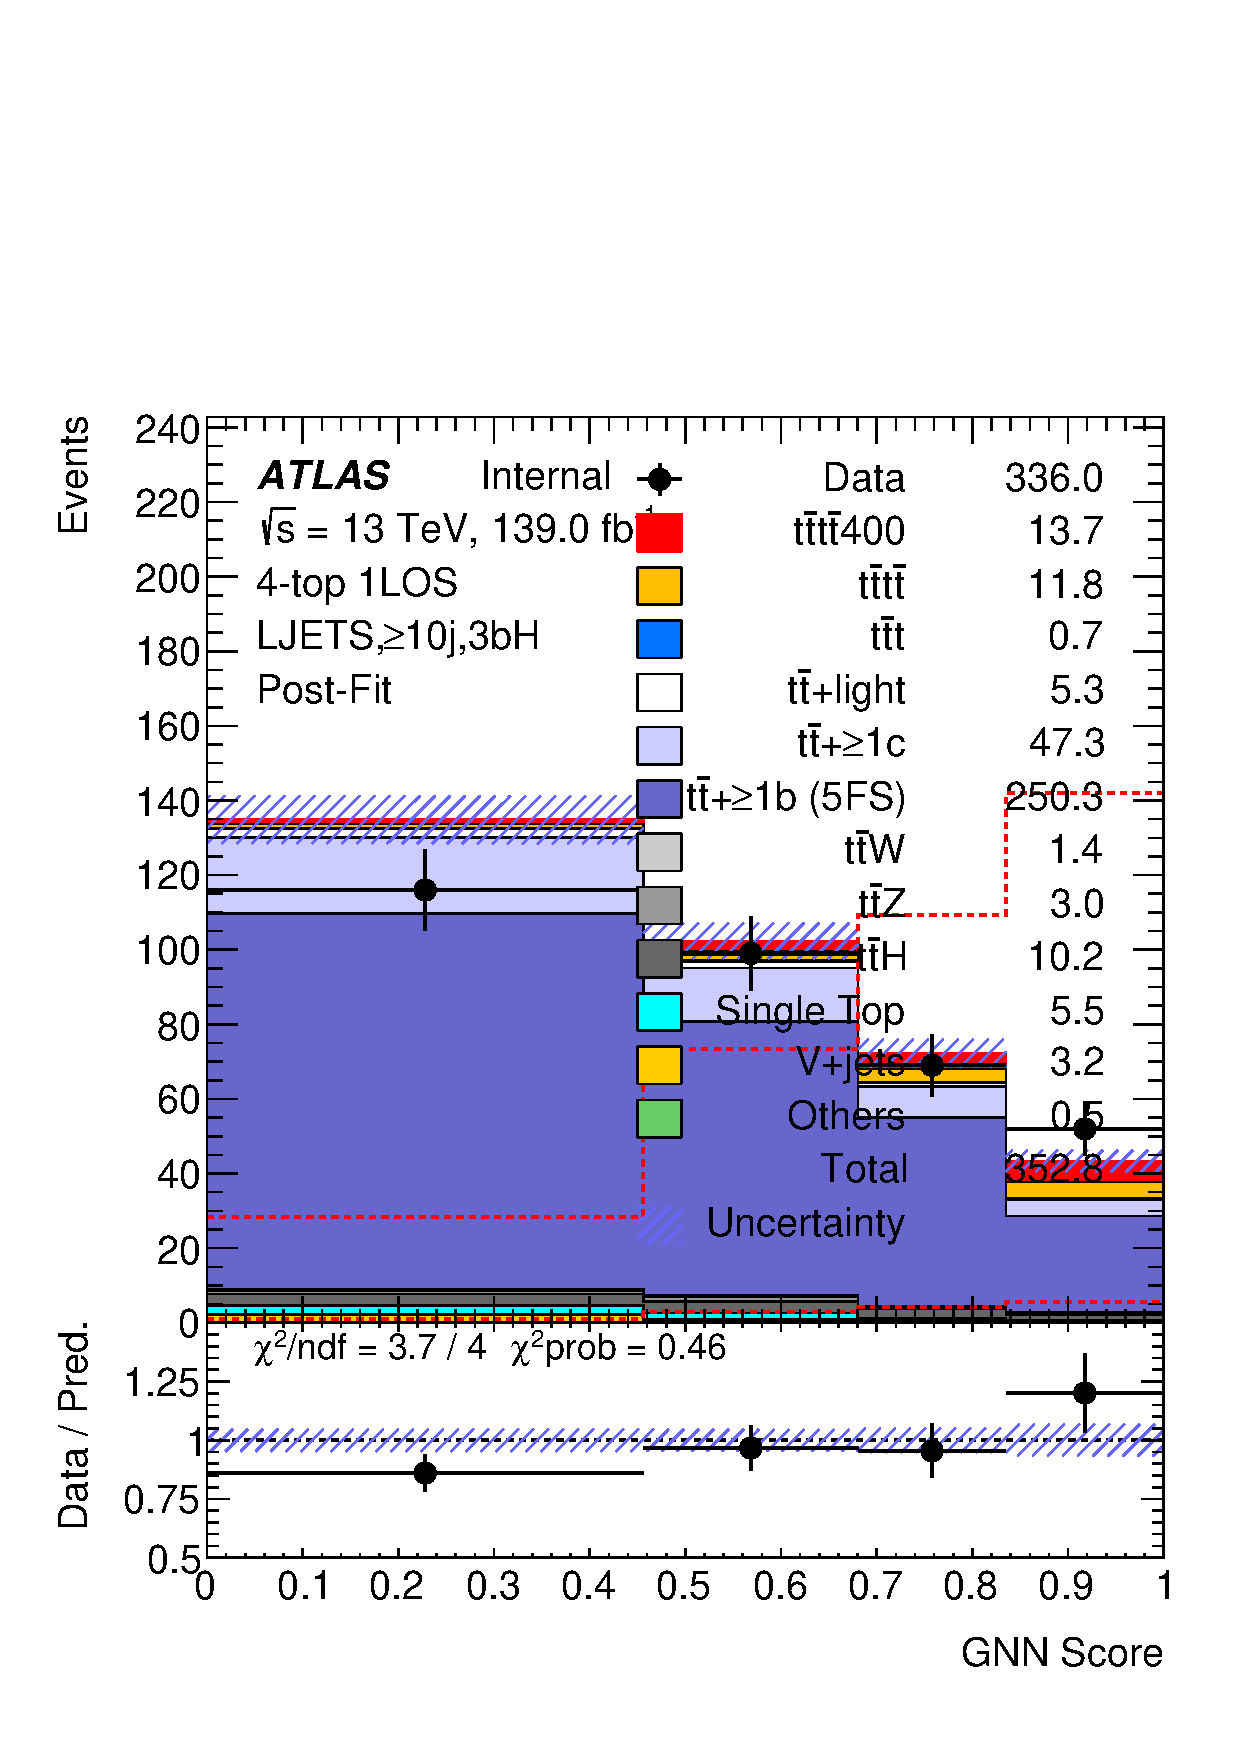
\includegraphics[width=0.23 \textwidth]{figures/fits/GNN/400/all/data_unblindedSplusB/Plots/ljets_ge10j3bH_postFit.pdf} &
        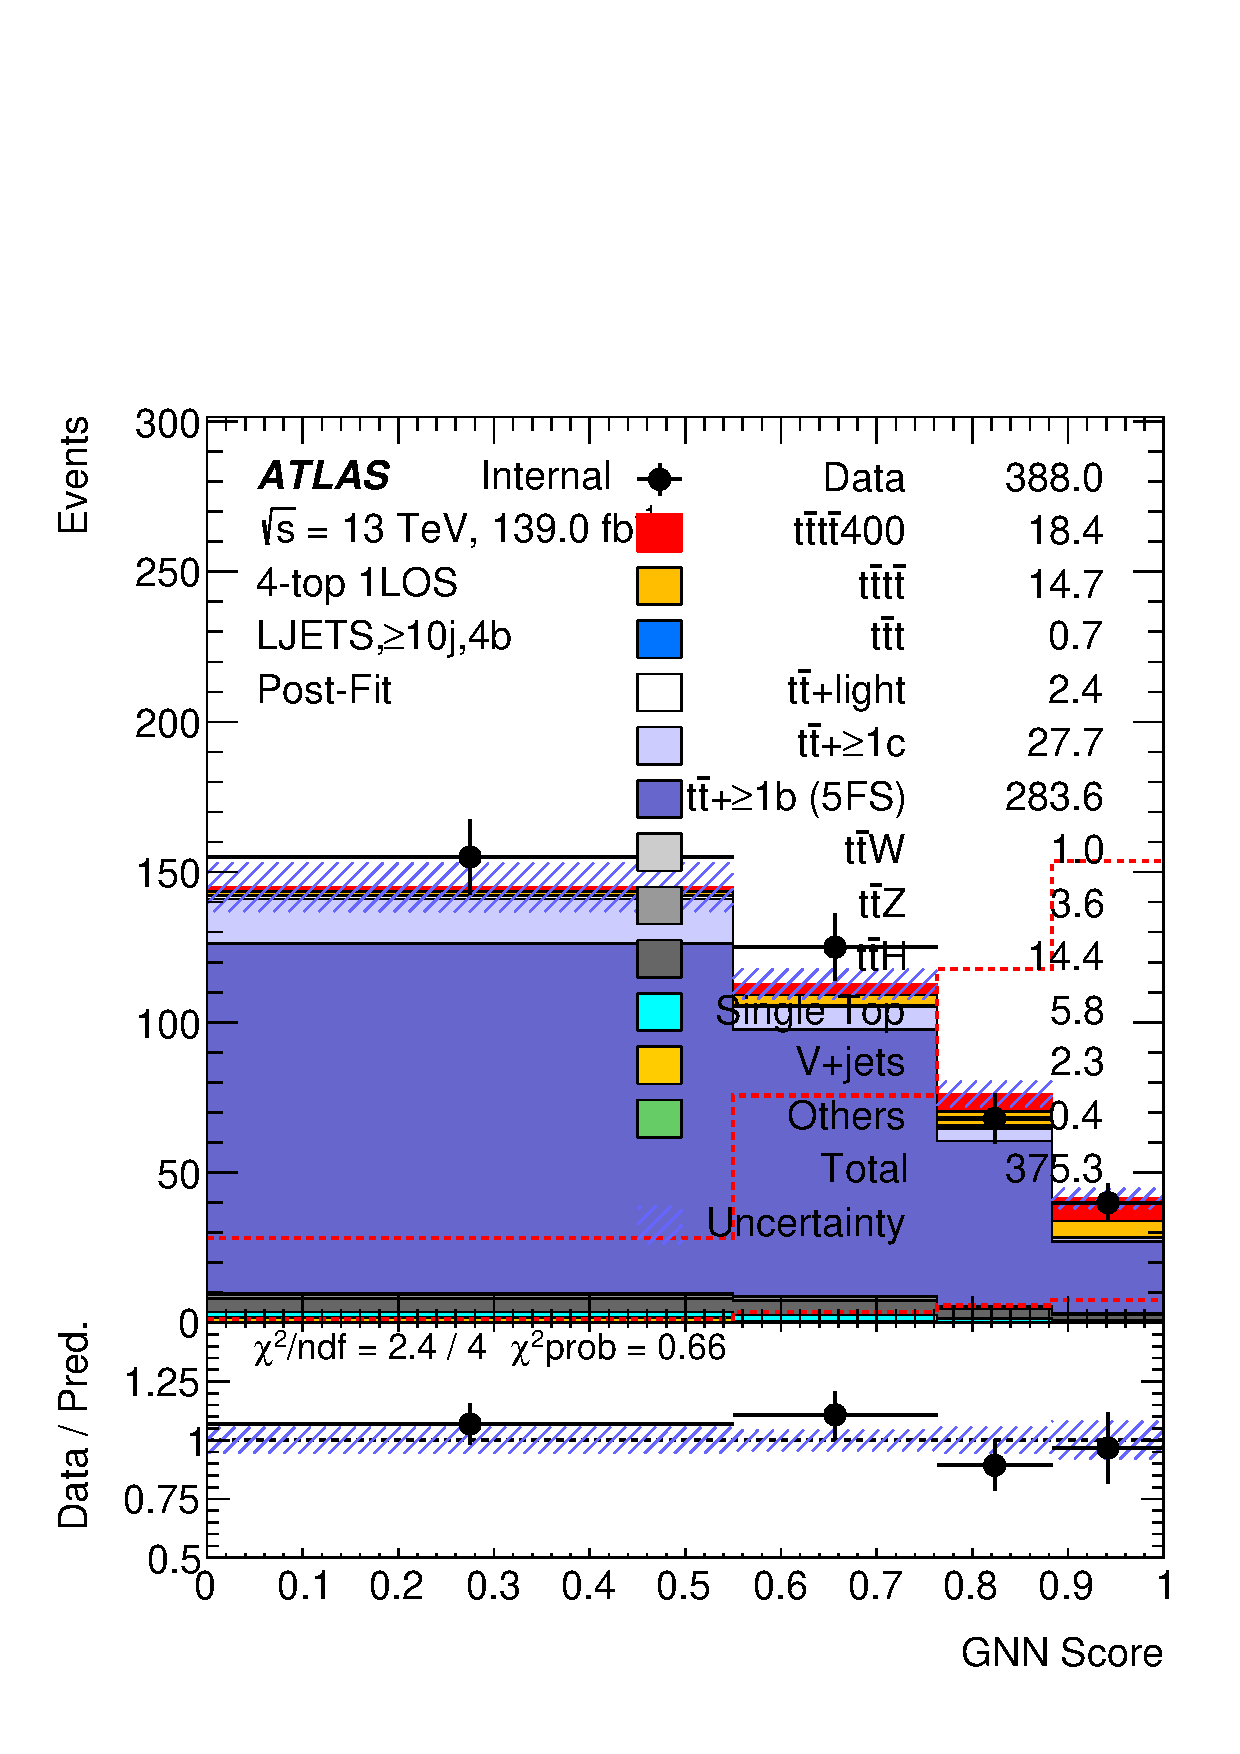
\includegraphics[width=0.23 \textwidth]{figures/fits/GNN/400/all/data_unblindedSplusB/Plots/ljets_ge10j4b_postFit.pdf} &
        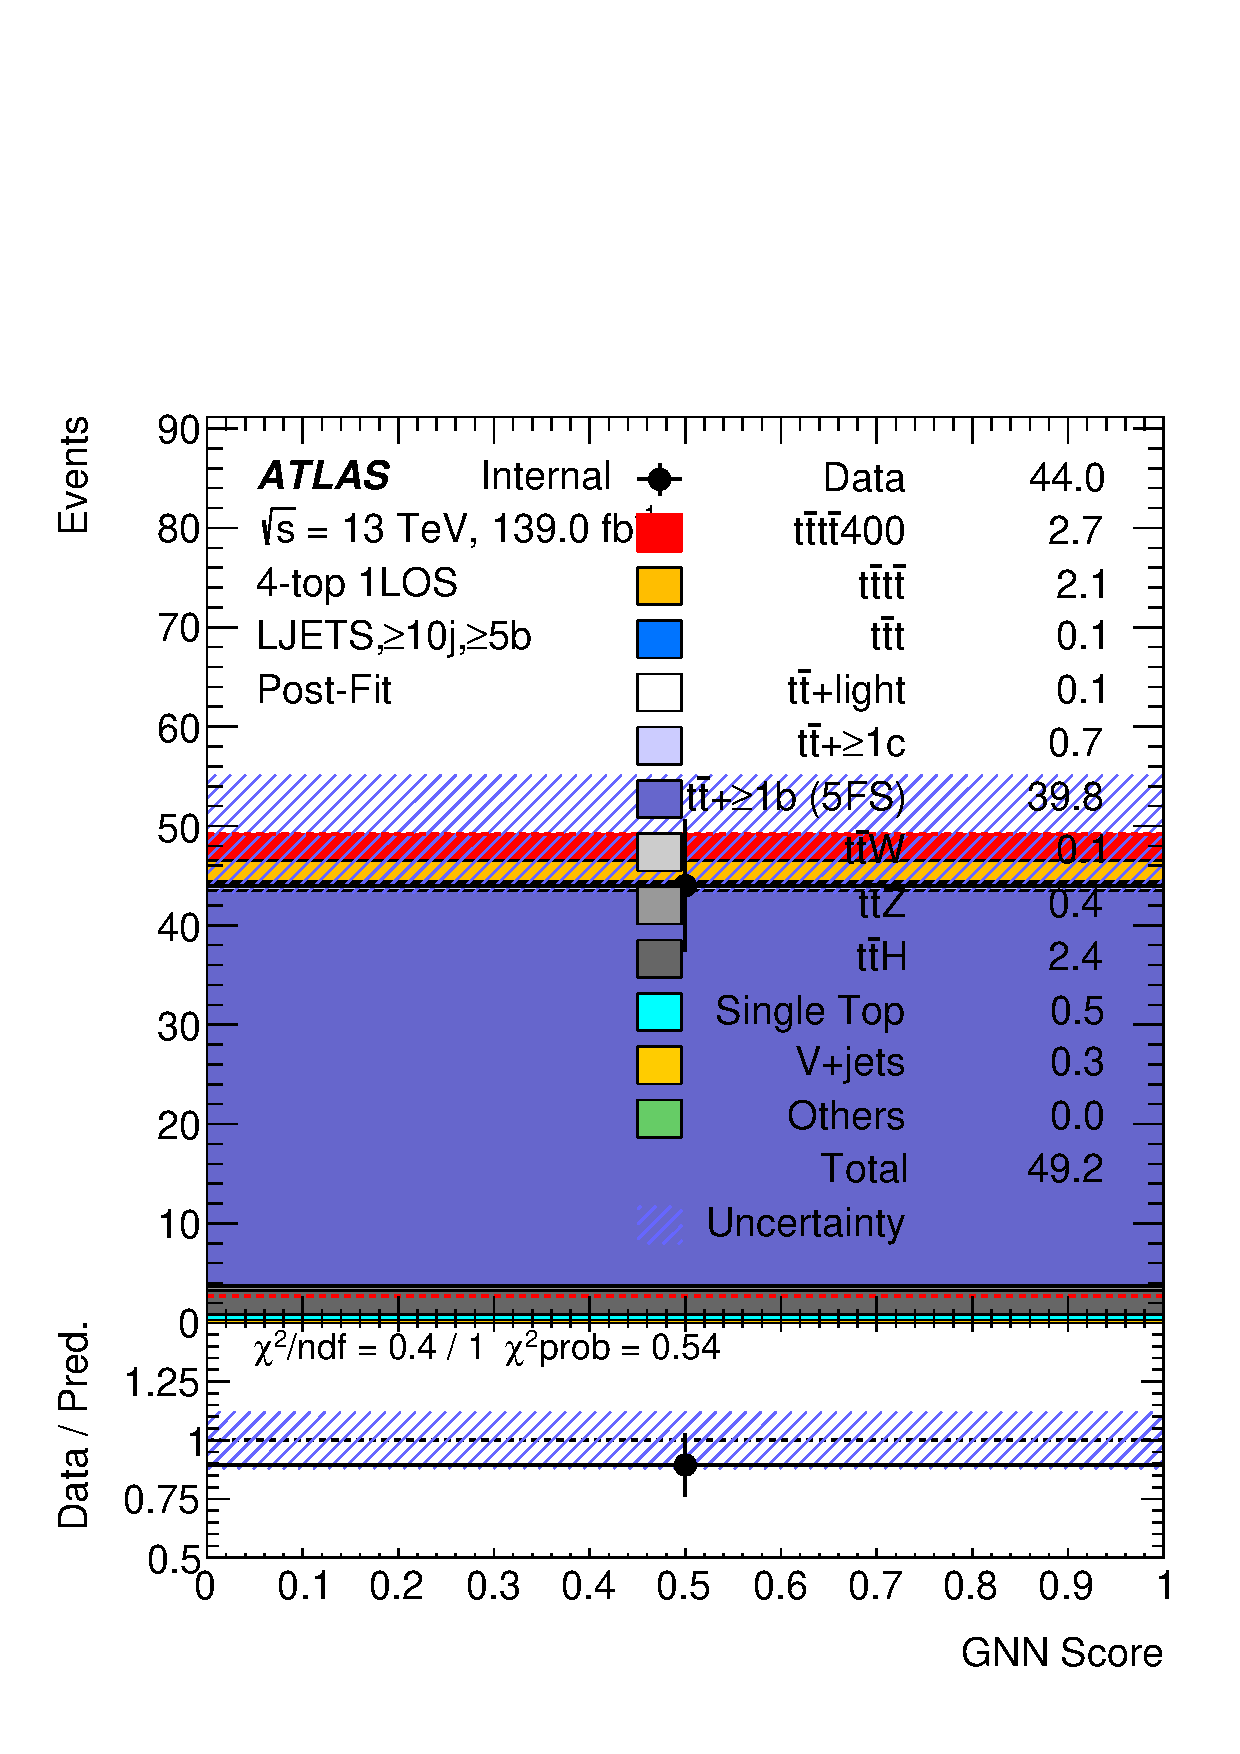
\includegraphics[width=0.23 \textwidth]{figures/fits/GNN/400/all/data_unblindedSplusB/Plots/ljets_ge10jge5b_postFit.pdf} \\
        \end{tabular}
        \caption{\label{fig:unblinded_data_SplusB_postfit_1L}Post-fit distributions for 1L regions obtained from unblinded signal+background data fit, compared with data yields for mH = 400 GeV. The fit is done using all regions (1L+2L).}
\end{center}
\end{figure}

\begin{figure}[htbp!]
        \begin{center} \setlength{\tabcolsep}{2.5pt}\footnotesize
        \begin{tabular}{ccc}
        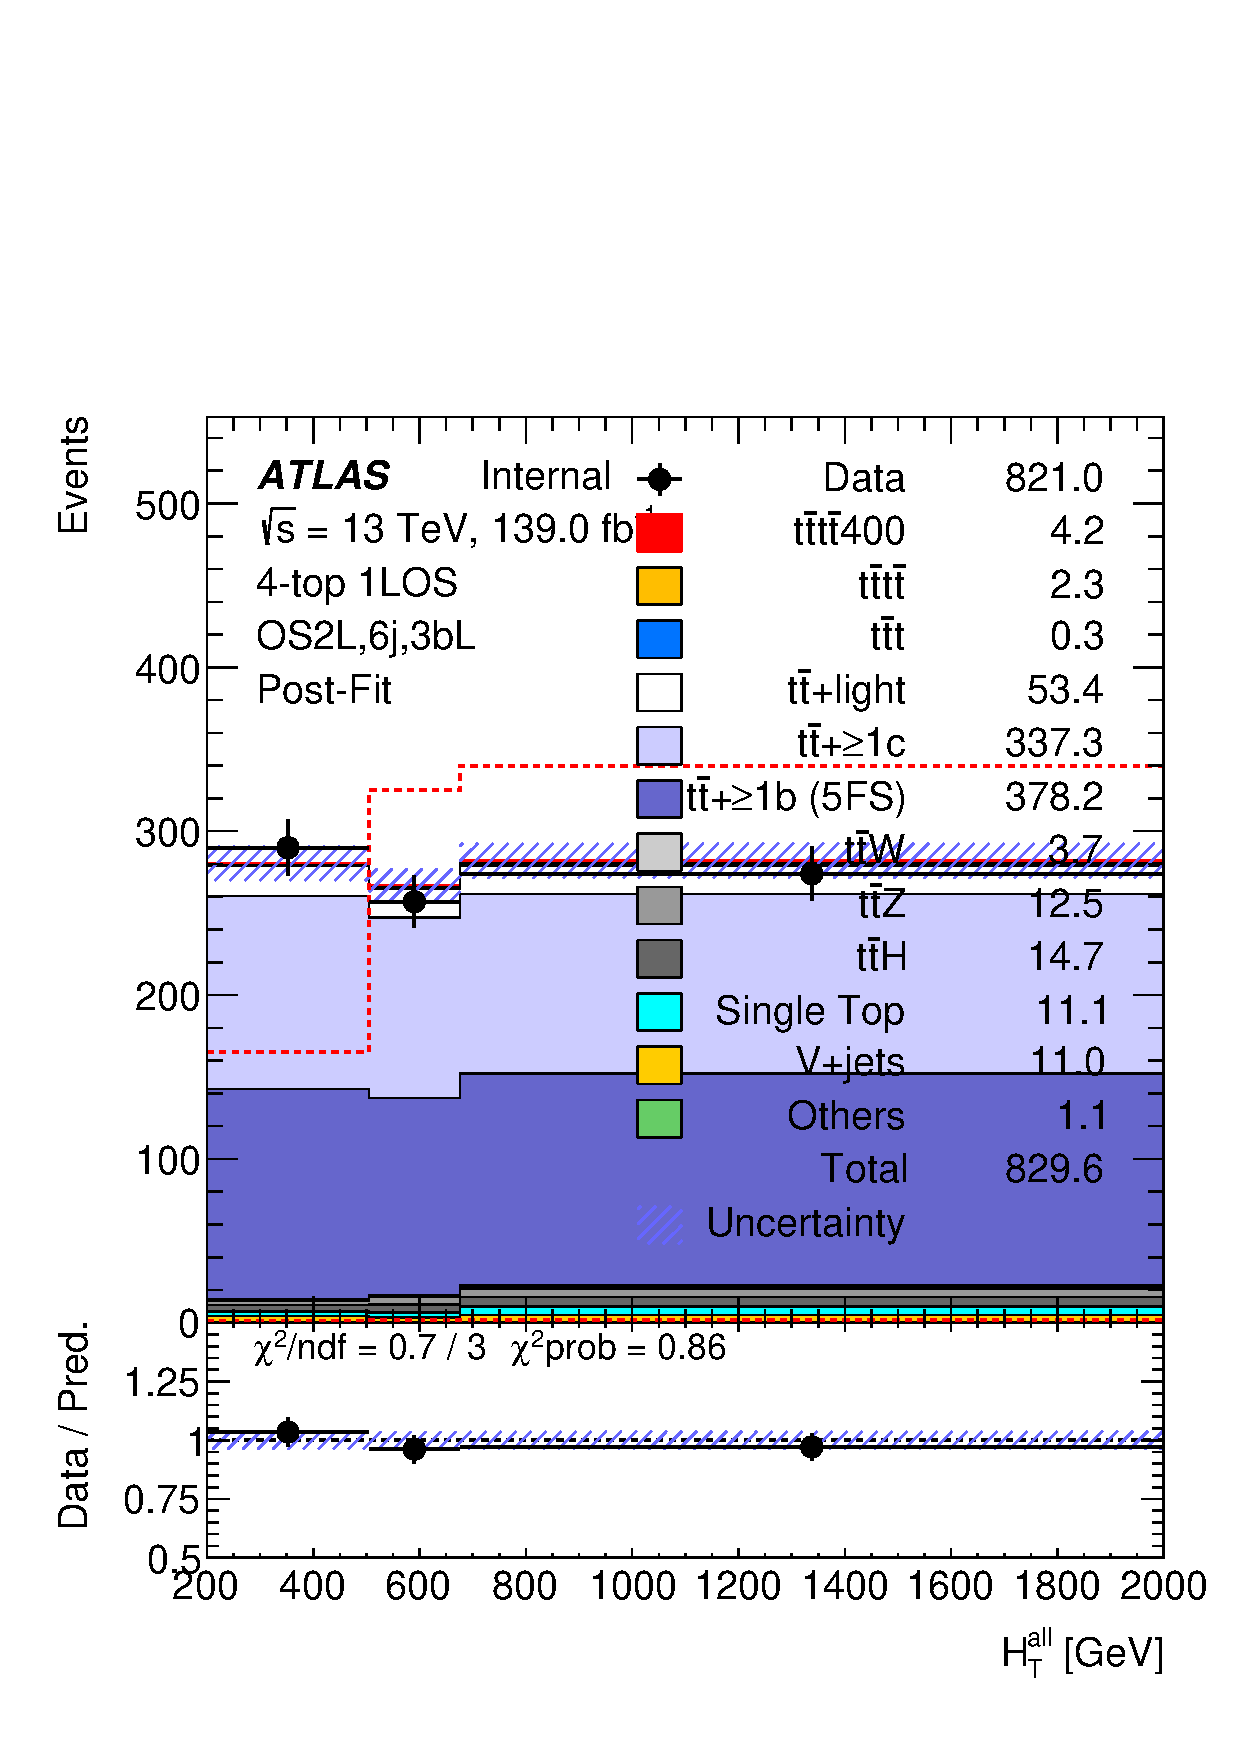
\includegraphics[width=0.31 \textwidth]{figures/fits/GNN/400/all/data_unblindedSplusB/Plots/os2l_6j3bL_postFit.pdf} &
        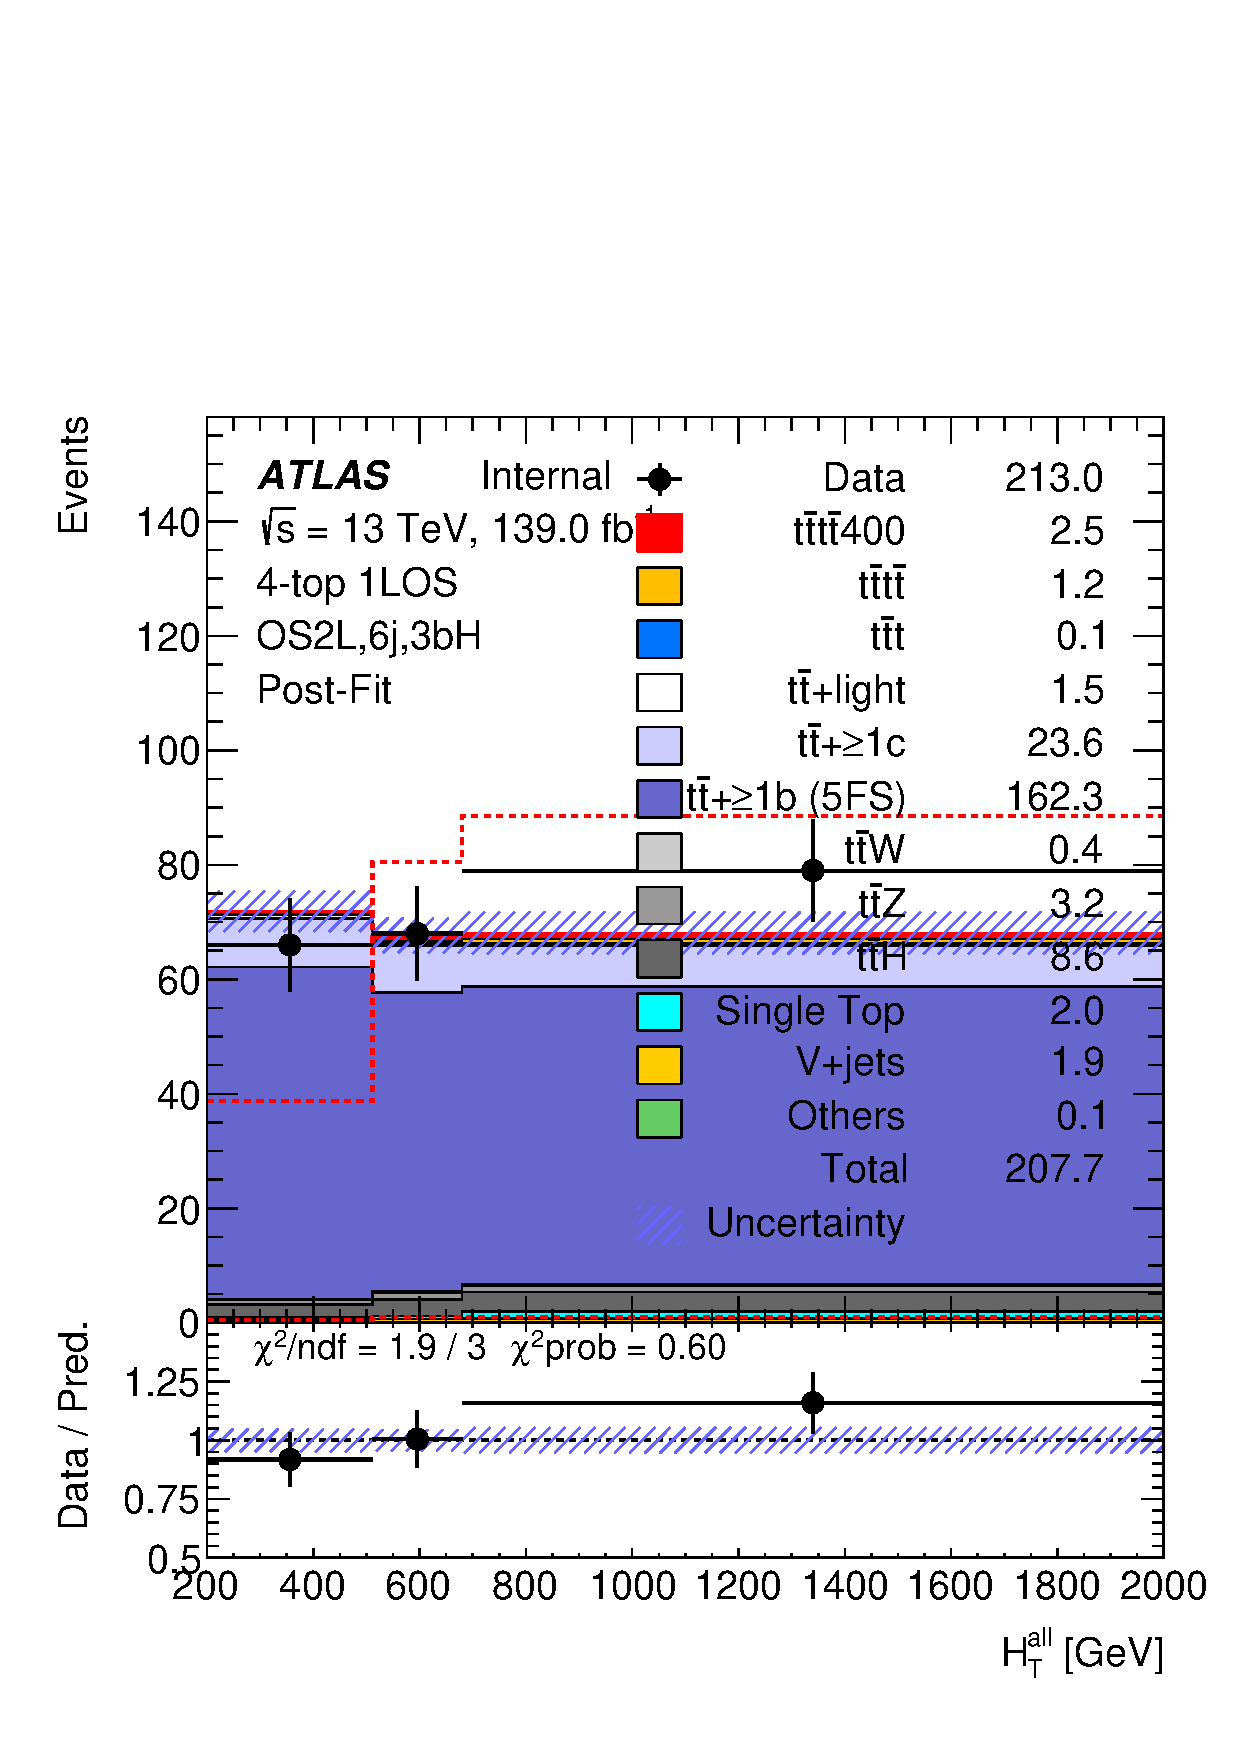
\includegraphics[width=0.31 \textwidth]{figures/fits/GNN/400/all/data_unblindedSplusB/Plots/os2l_6j3bH_postFit.pdf} &
        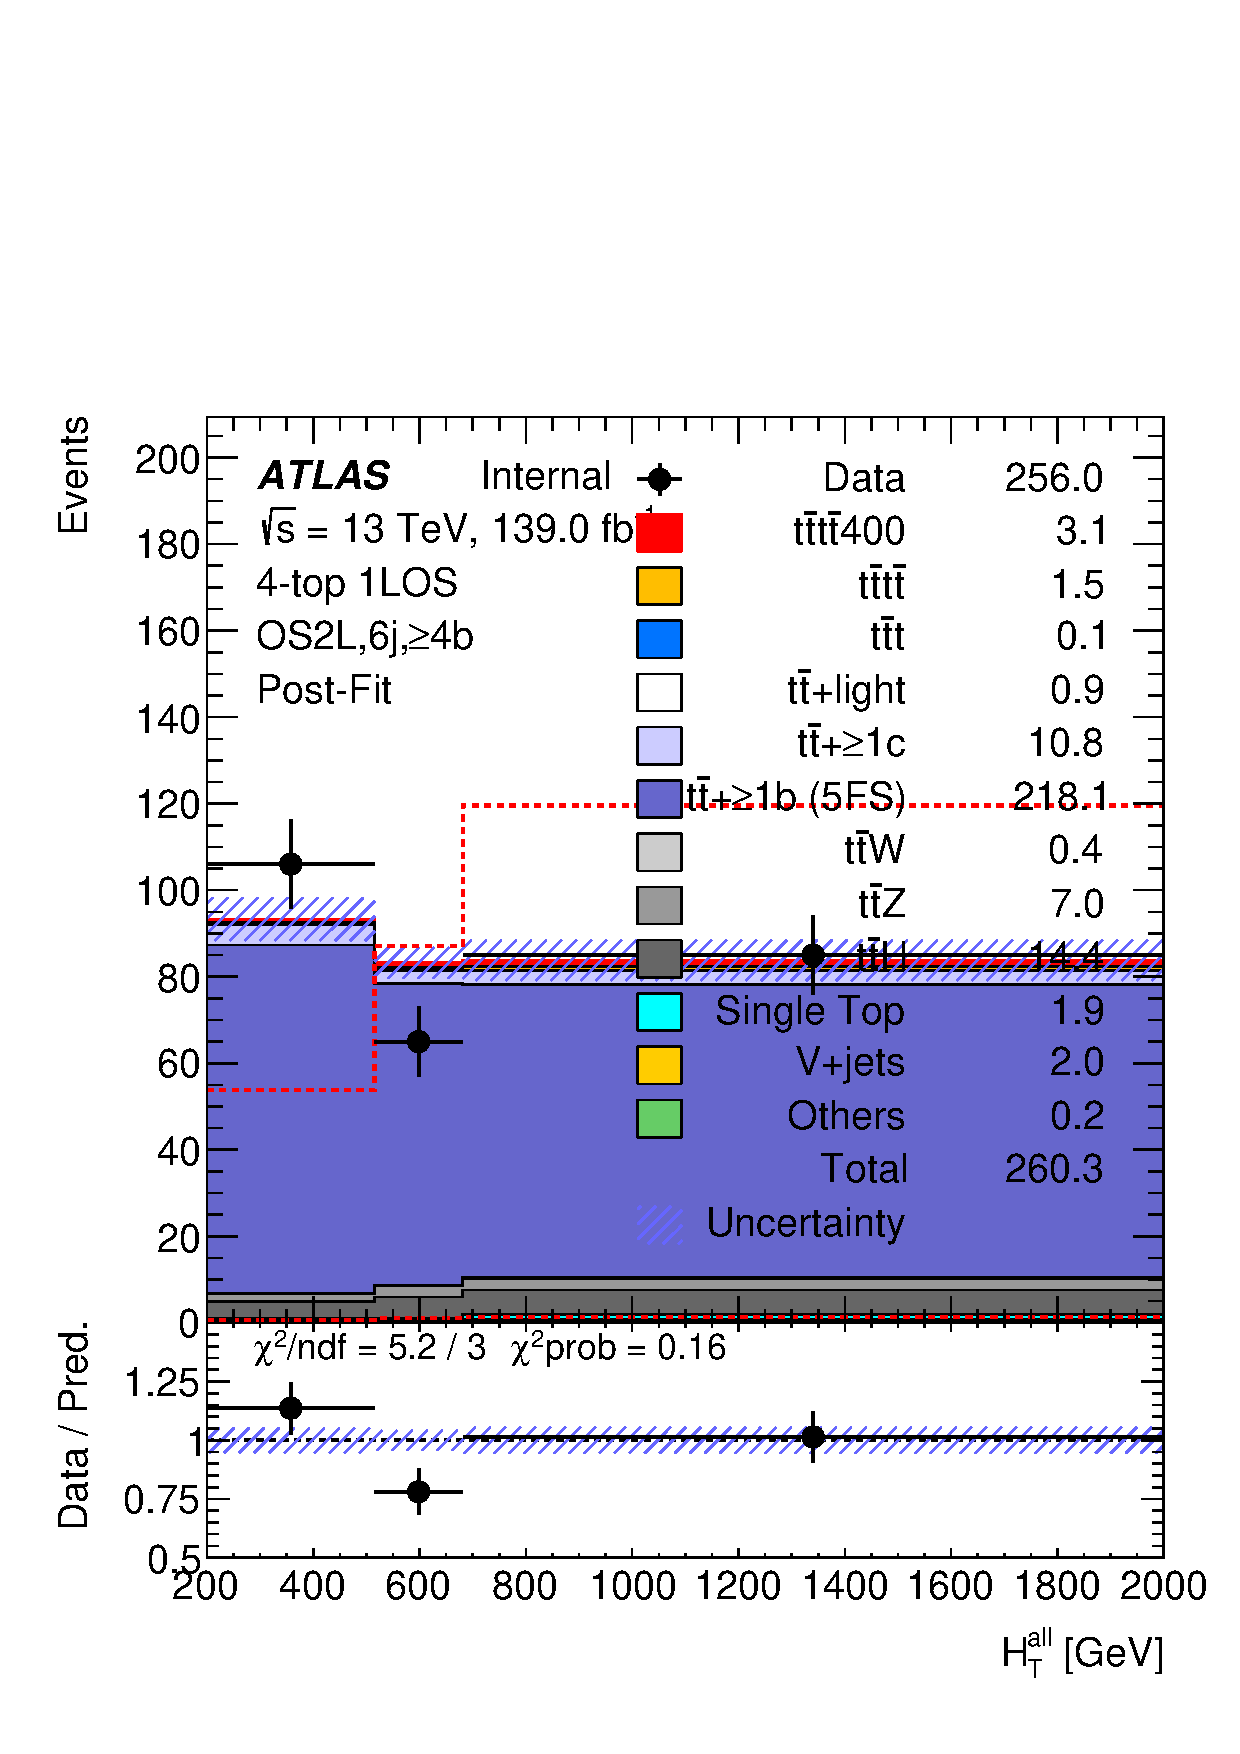
\includegraphics[width=0.31 \textwidth]{figures/fits/GNN/400/all/data_unblindedSplusB/Plots/os2l_6jge4b_postFit.pdf} \\

        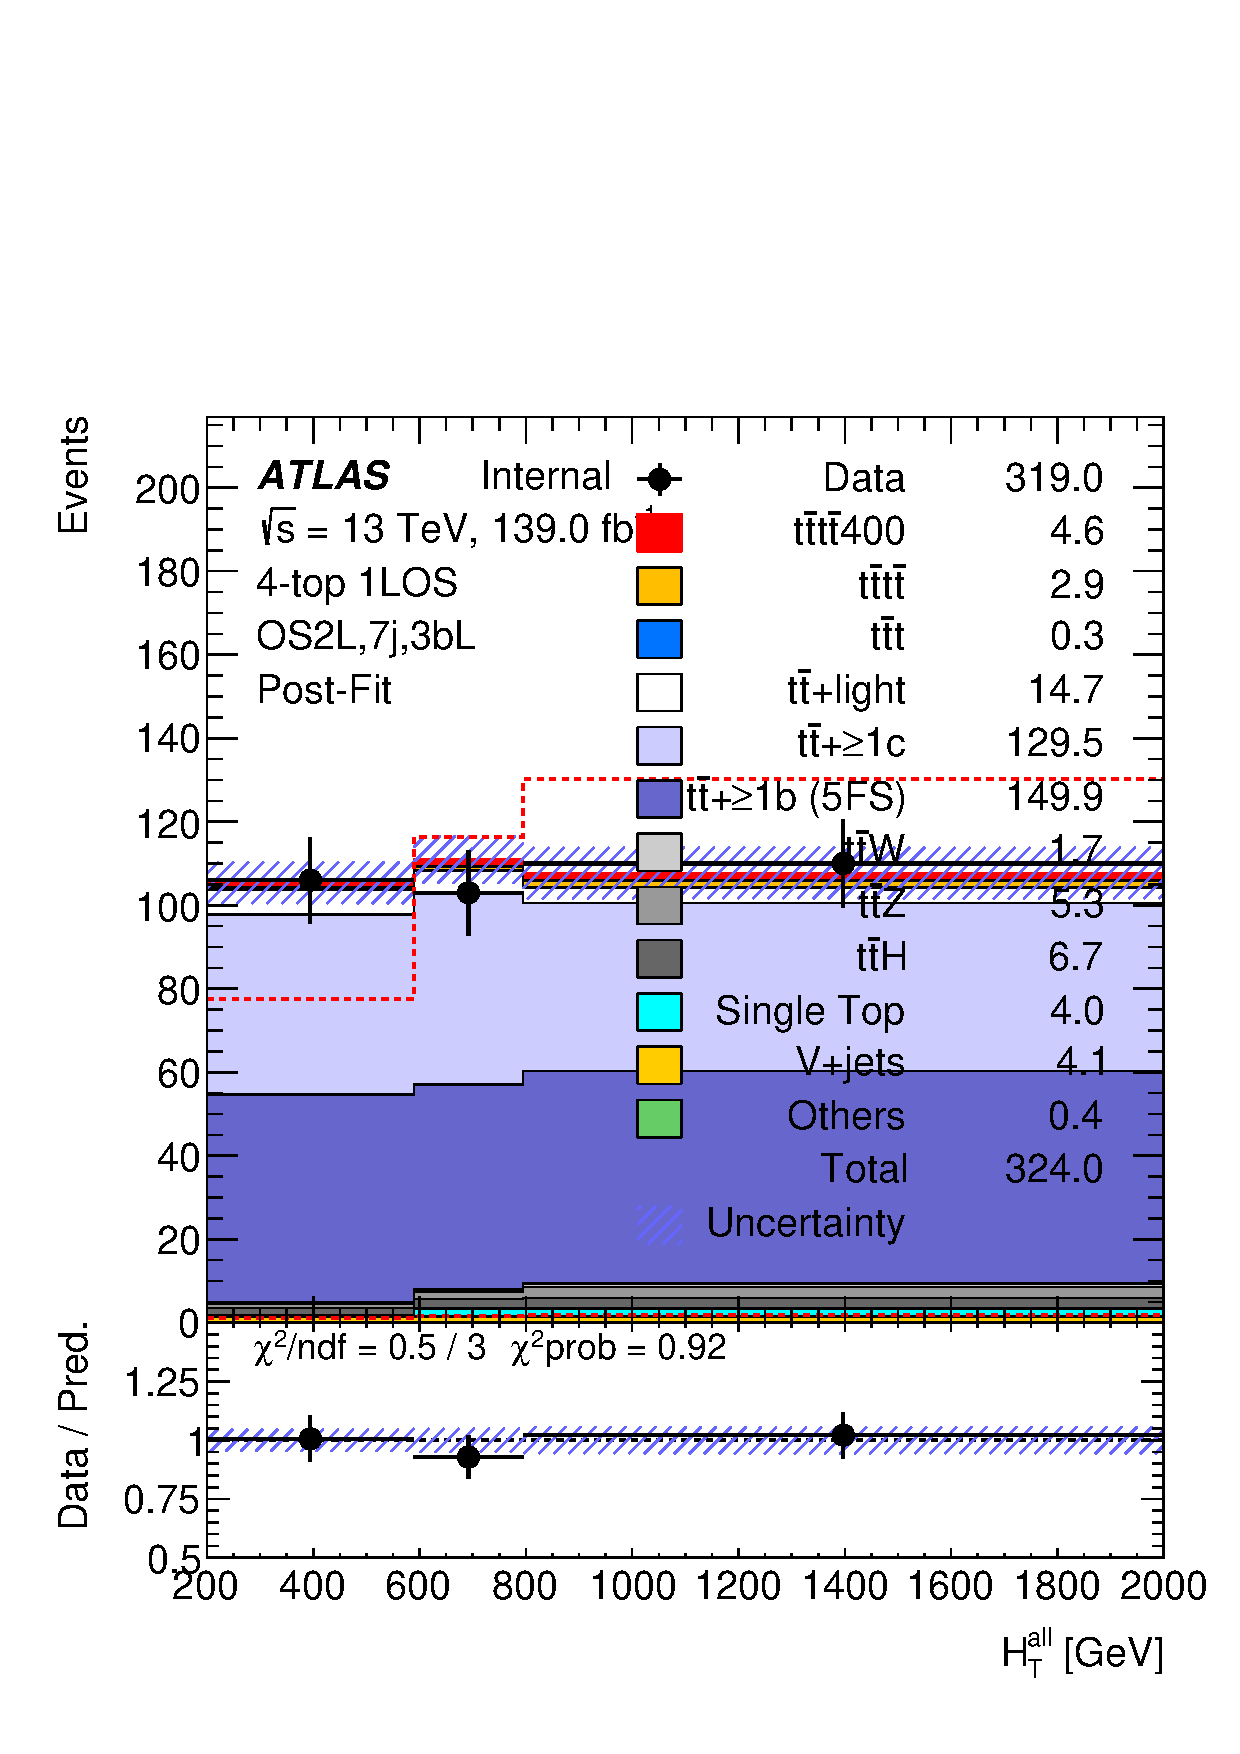
\includegraphics[width=0.31 \textwidth]{figures/fits/GNN/400/all/data_unblindedSplusB/Plots/os2l_7j3bL_postFit.pdf} &
        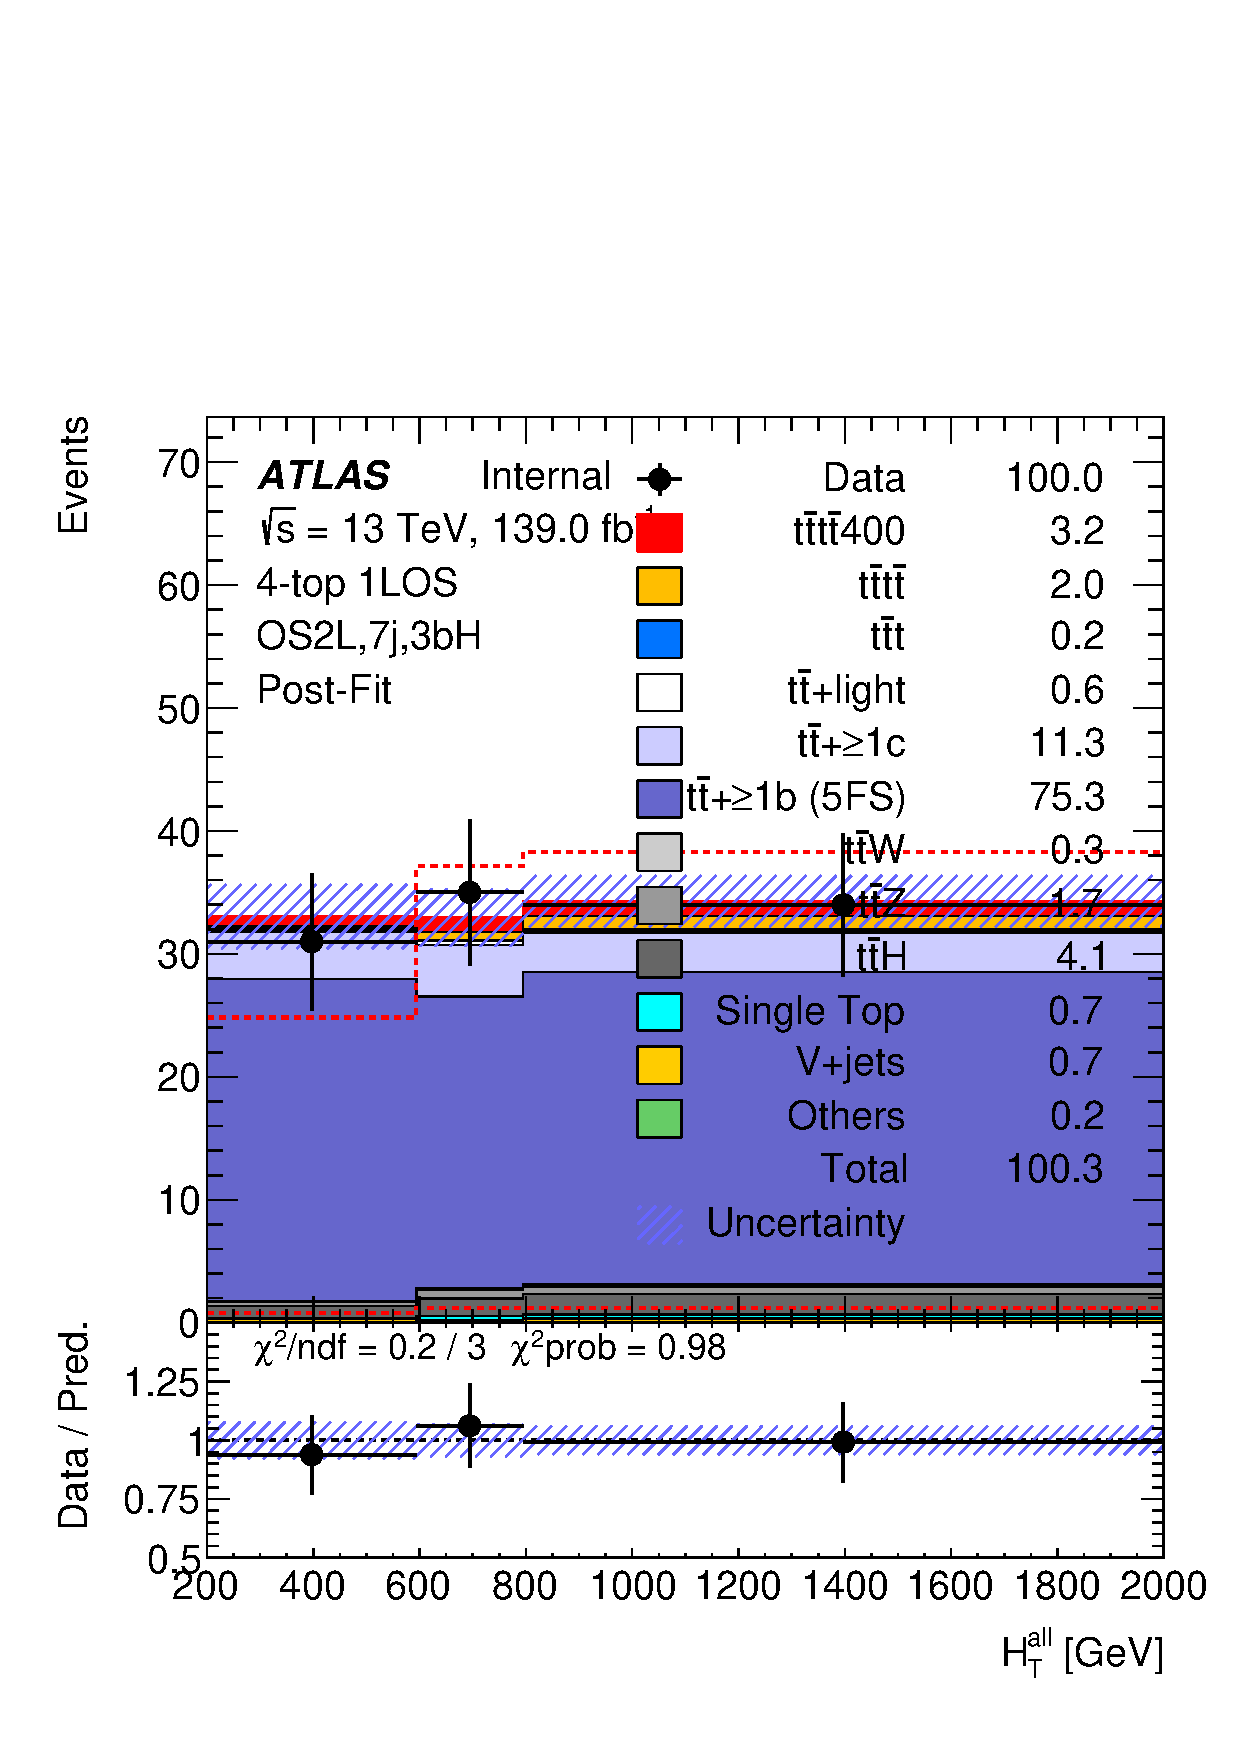
\includegraphics[width=0.31 \textwidth]{figures/fits/GNN/400/all/data_unblindedSplusB/Plots/os2l_7j3bH_postFit.pdf} &
        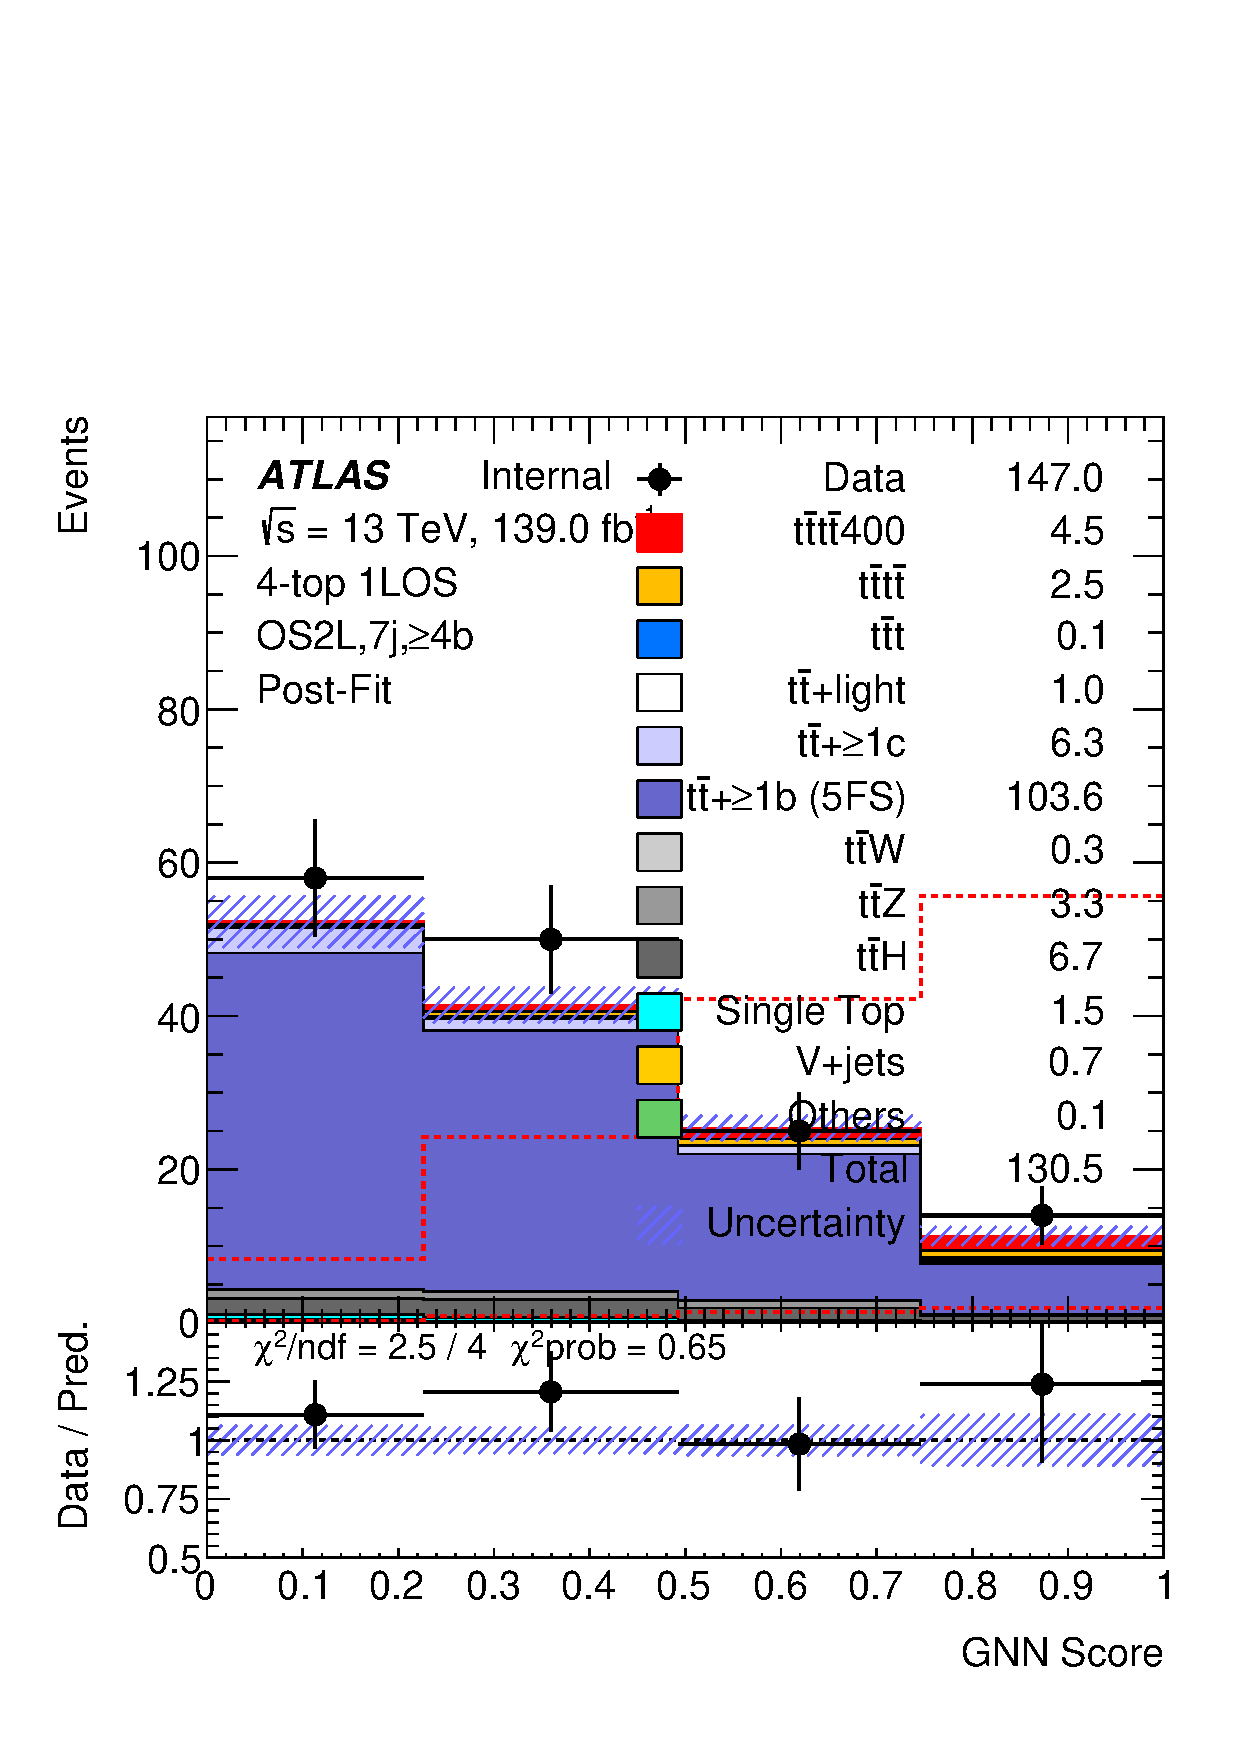
\includegraphics[width=0.31 \textwidth]{figures/fits/GNN/400/all/data_unblindedSplusB/Plots/os2l_7jge4b_postFit.pdf} \\

        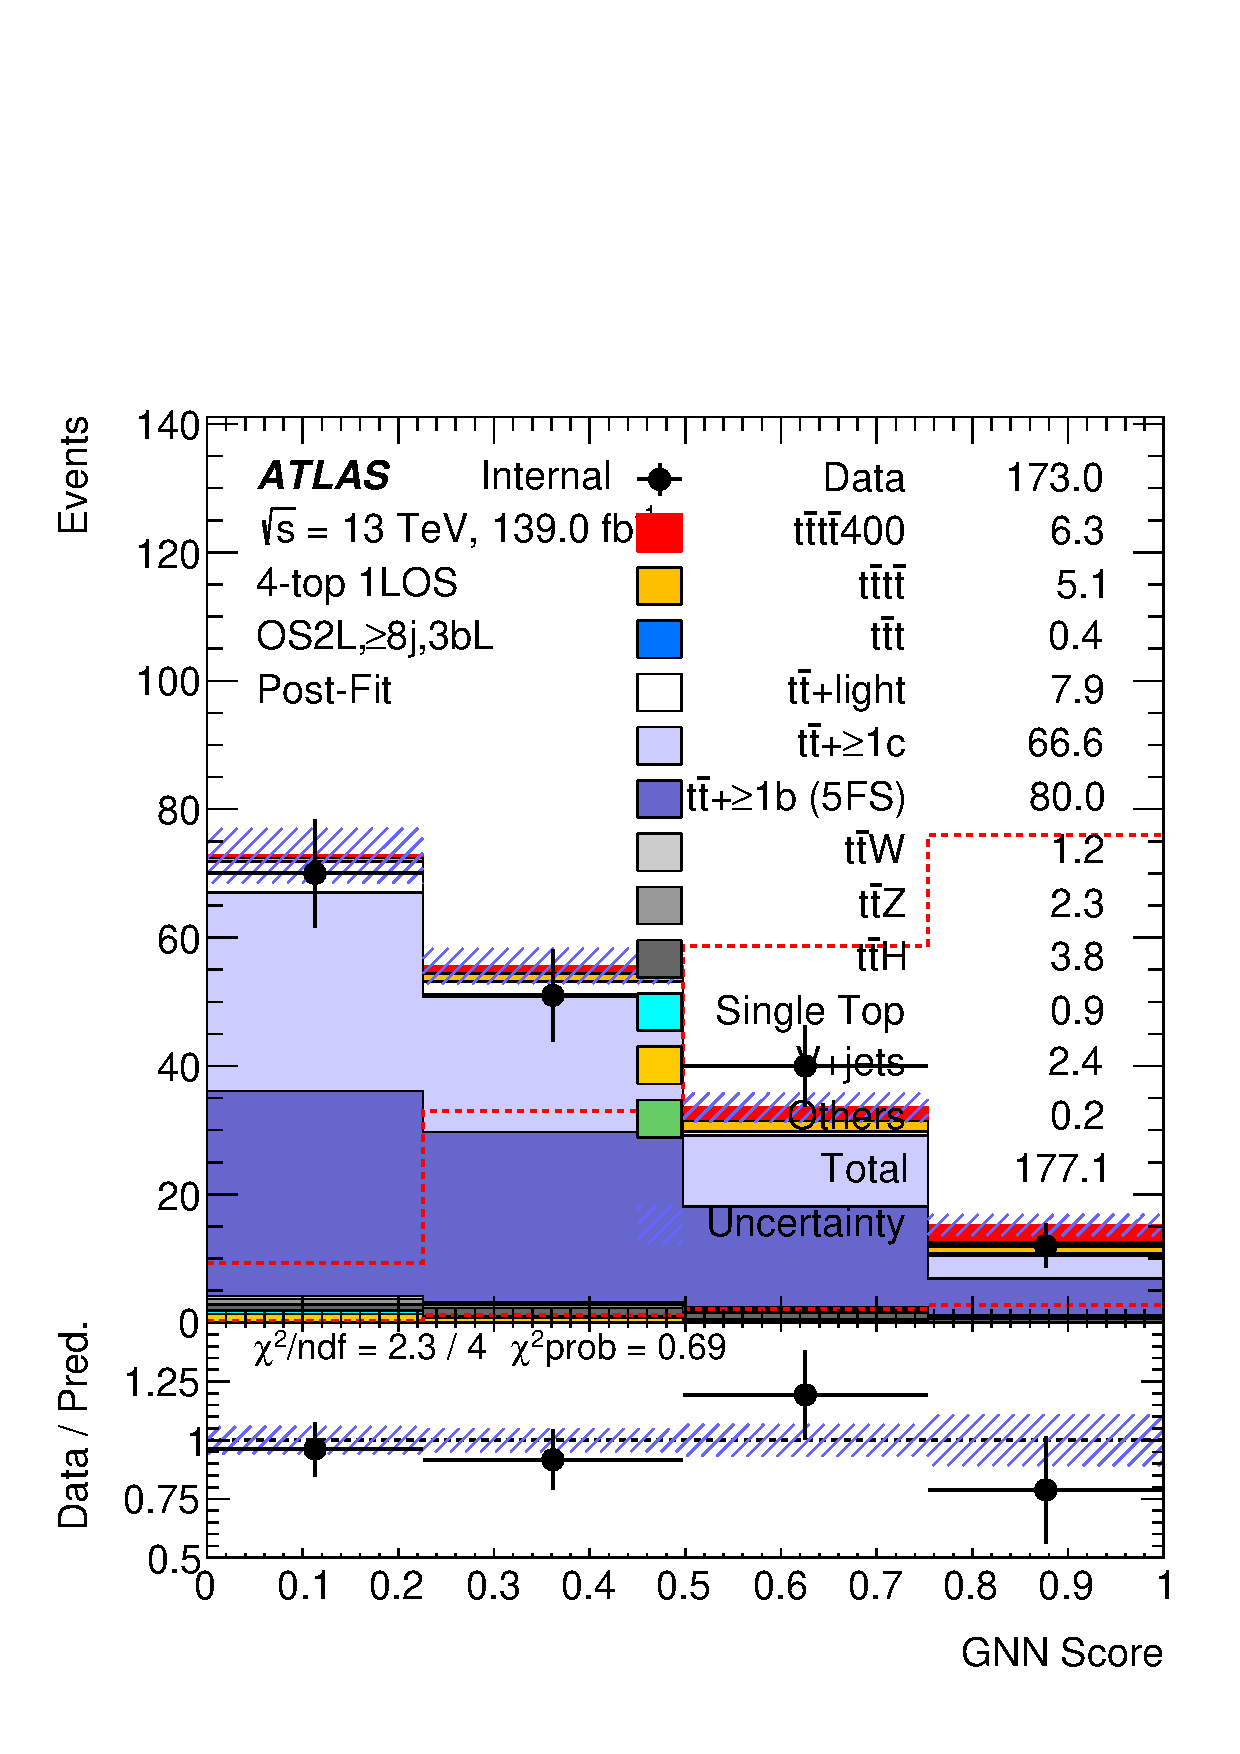
\includegraphics[width=0.31 \textwidth]{figures/fits/GNN/400/all/data_unblindedSplusB/Plots/os2l_ge8j3bL_postFit.pdf} &
        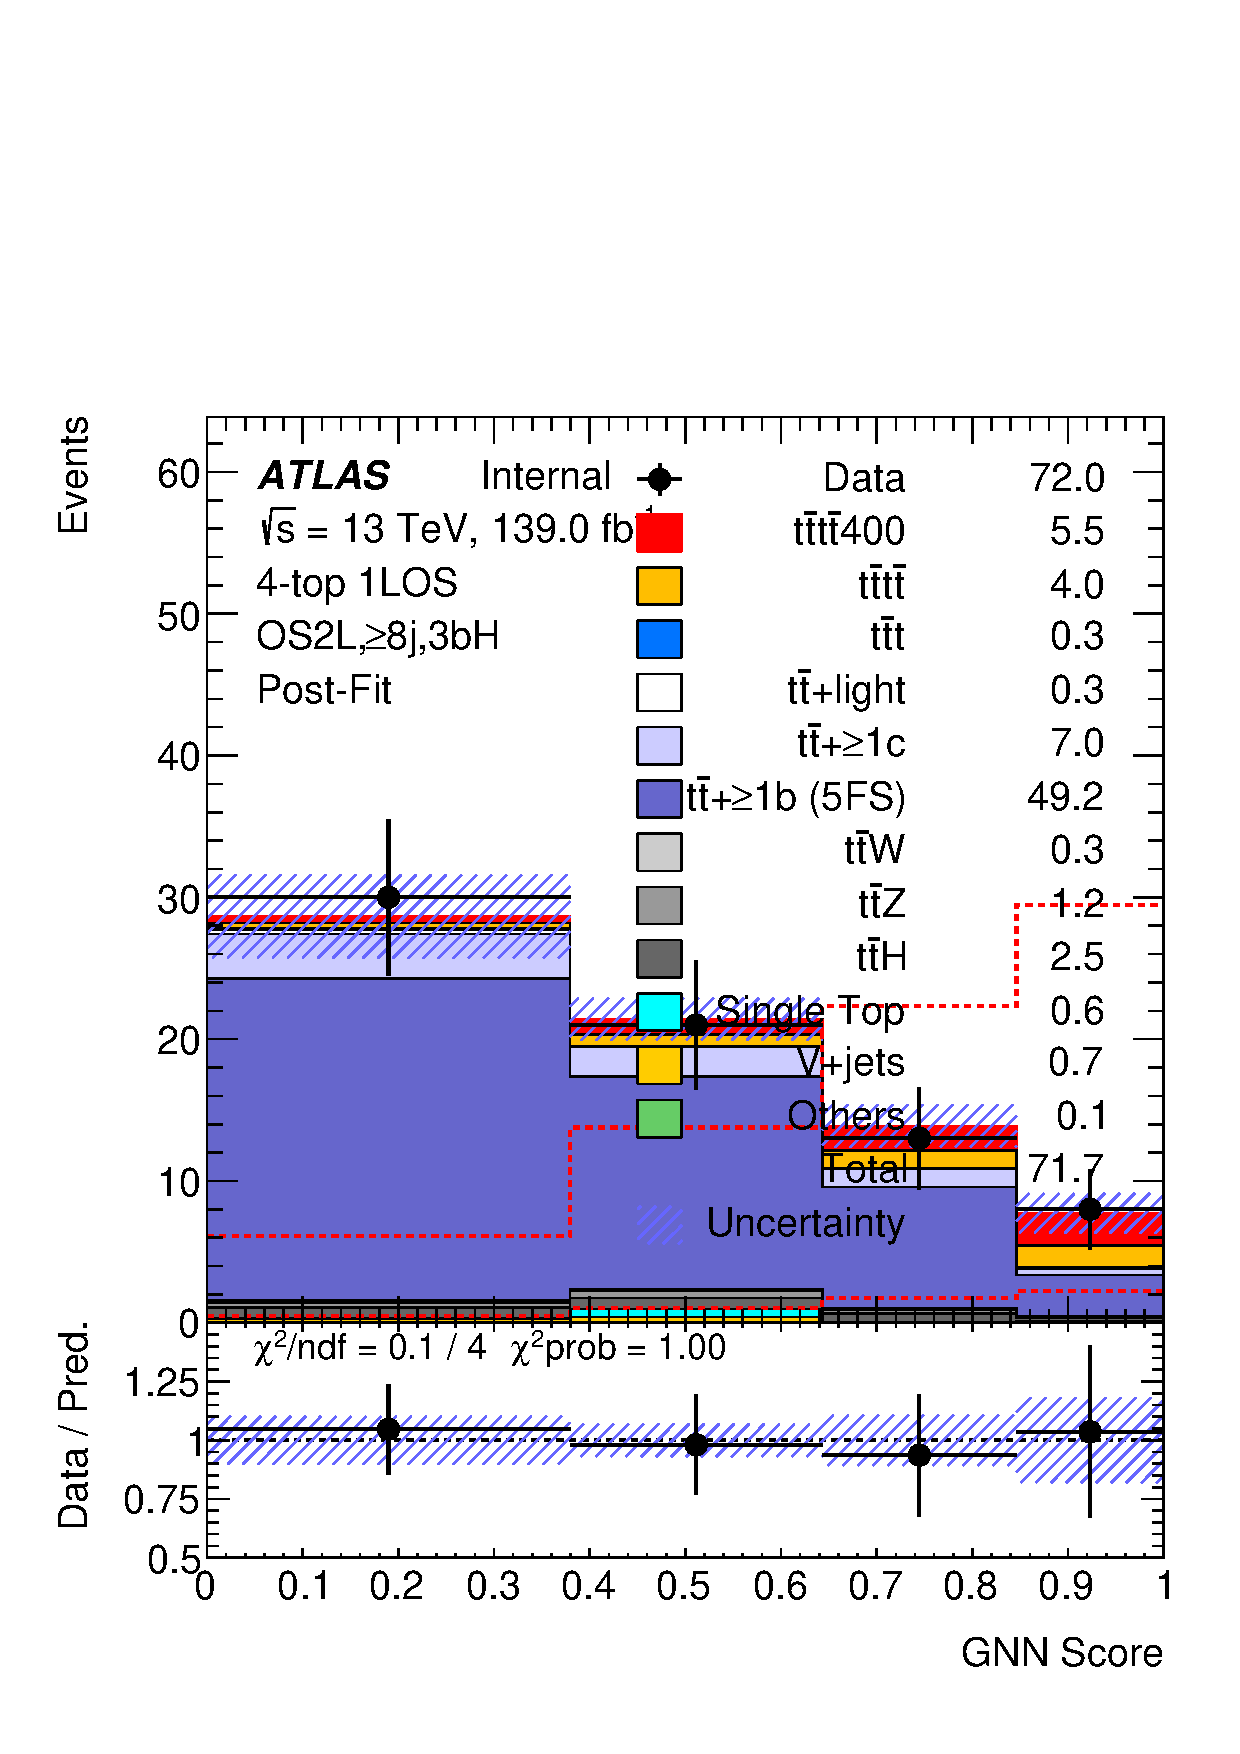
\includegraphics[width=0.31 \textwidth]{figures/fits/GNN/400/all/data_unblindedSplusB/Plots/os2l_ge8j3bH_postFit.pdf} &
        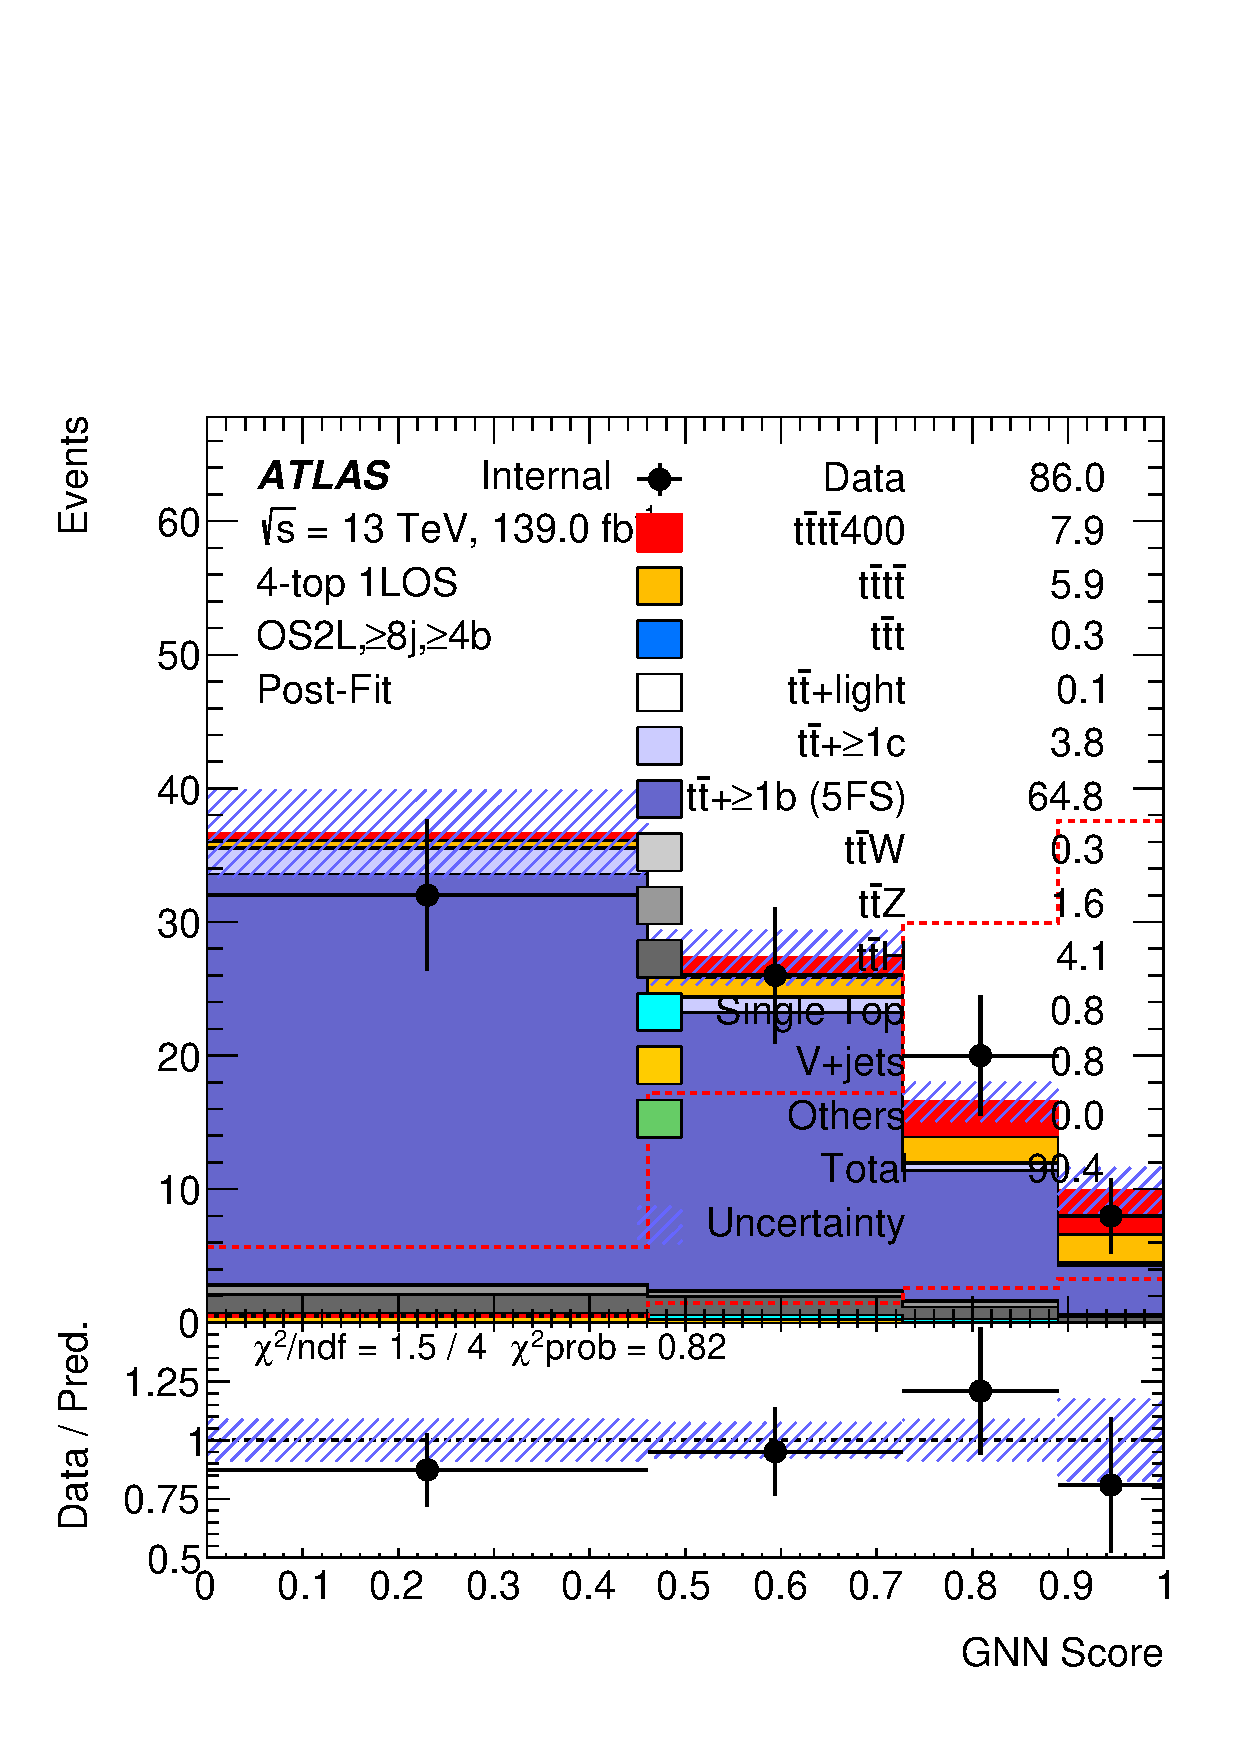
\includegraphics[width=0.31 \textwidth]{figures/fits/GNN/400/all/data_unblindedSplusB/Plots/os2l_ge8jge4b_postFit.pdf} \\
        \end{tabular}
        \caption{\label{fig:unblinded_data_SplusB_postfit_2L}Post-fit distributions for 2LOS regions obtained from unblinded signal+background data fit, compared with data yields for mH = 400 GeV. The fit is done using all regions (1L+2L)}
\end{center}
\end{figure}


\begin{figure}[htbp!]
  \centering
  \begin{subfigure}[t]{0.32\textwidth}
    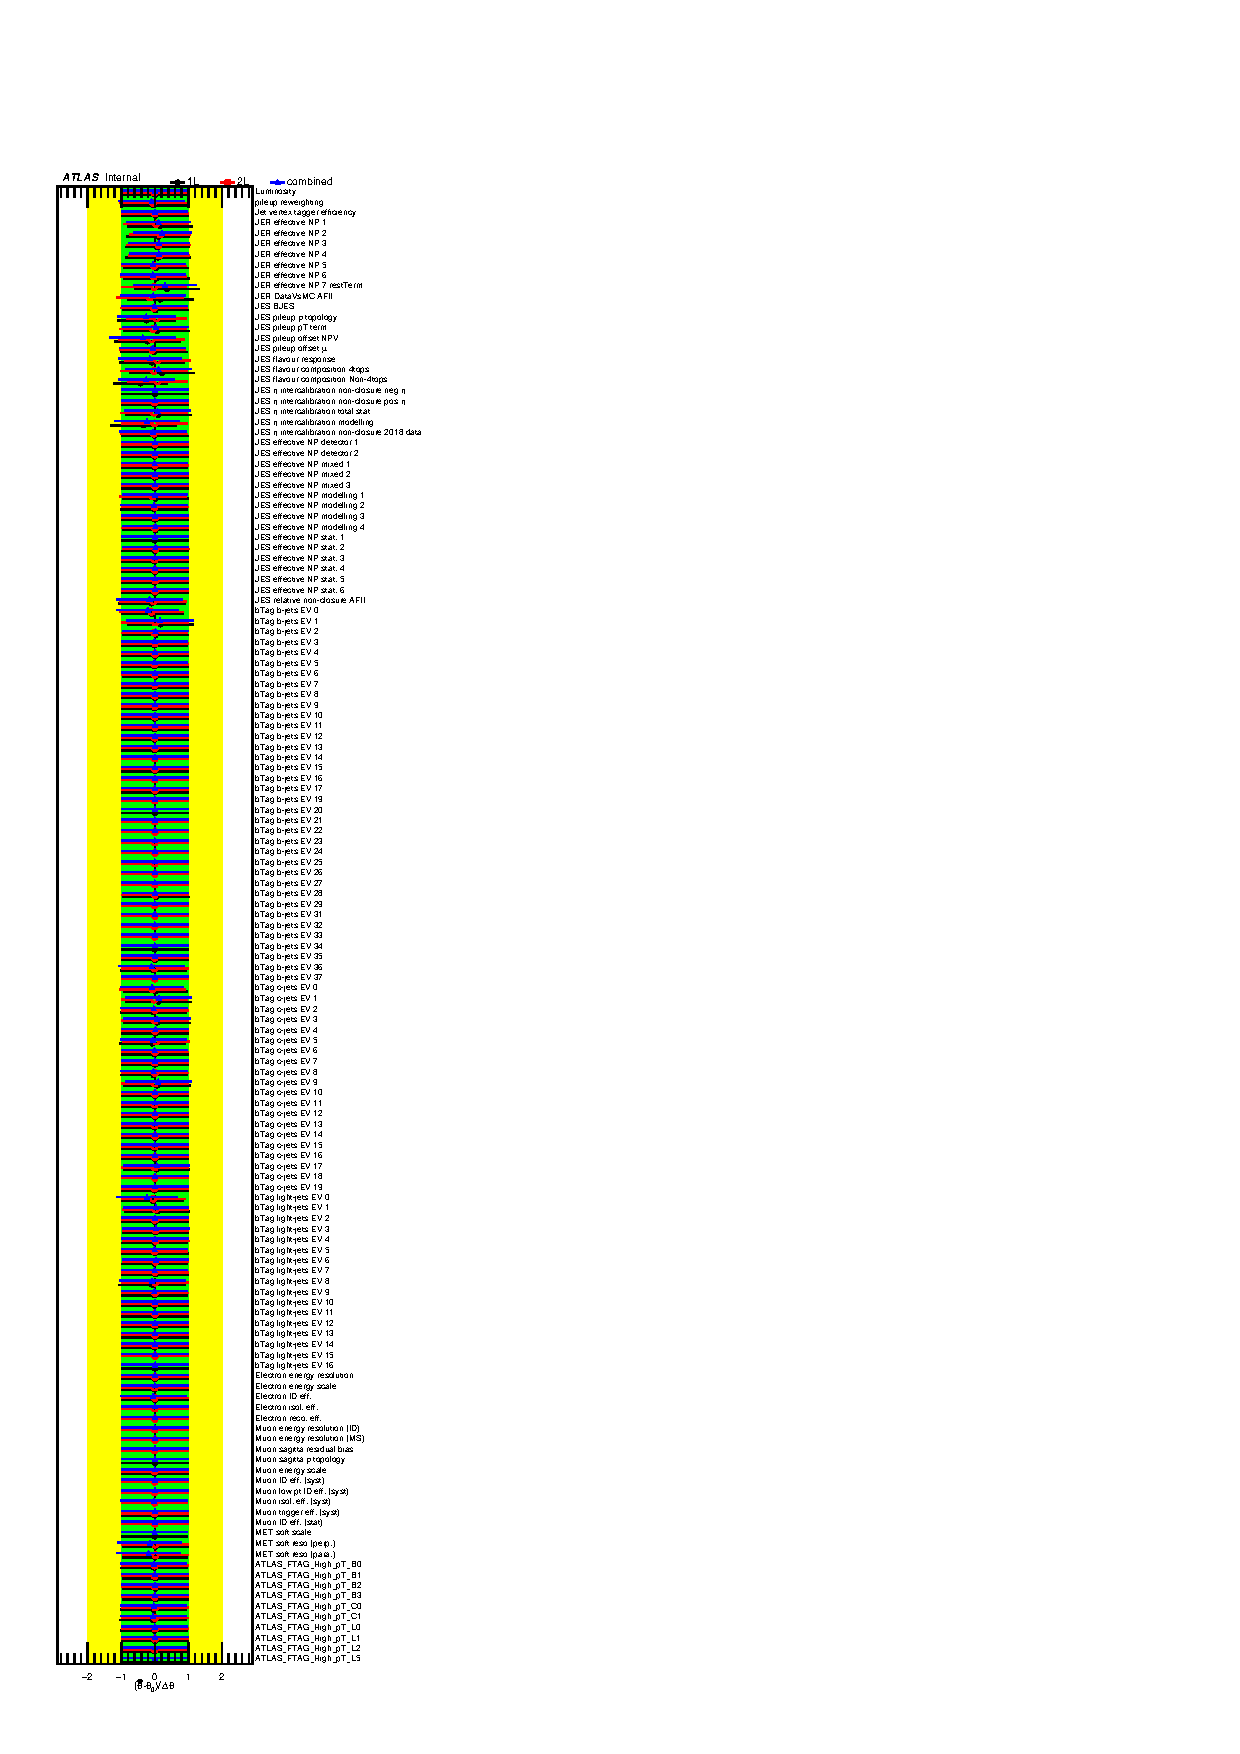
\includegraphics[width=\linewidth]{figures/fits/comparisons/selections/GNN/400/data_unblindedSplusB/NuisPar_comp_Instrumental.pdf}
    \subcaption{mH=400\gev}
    \label{fig:unblinded_data_SplusB_NP_mH400}
  \end{subfigure}
  \begin{subfigure}[t]{0.32\textwidth}
    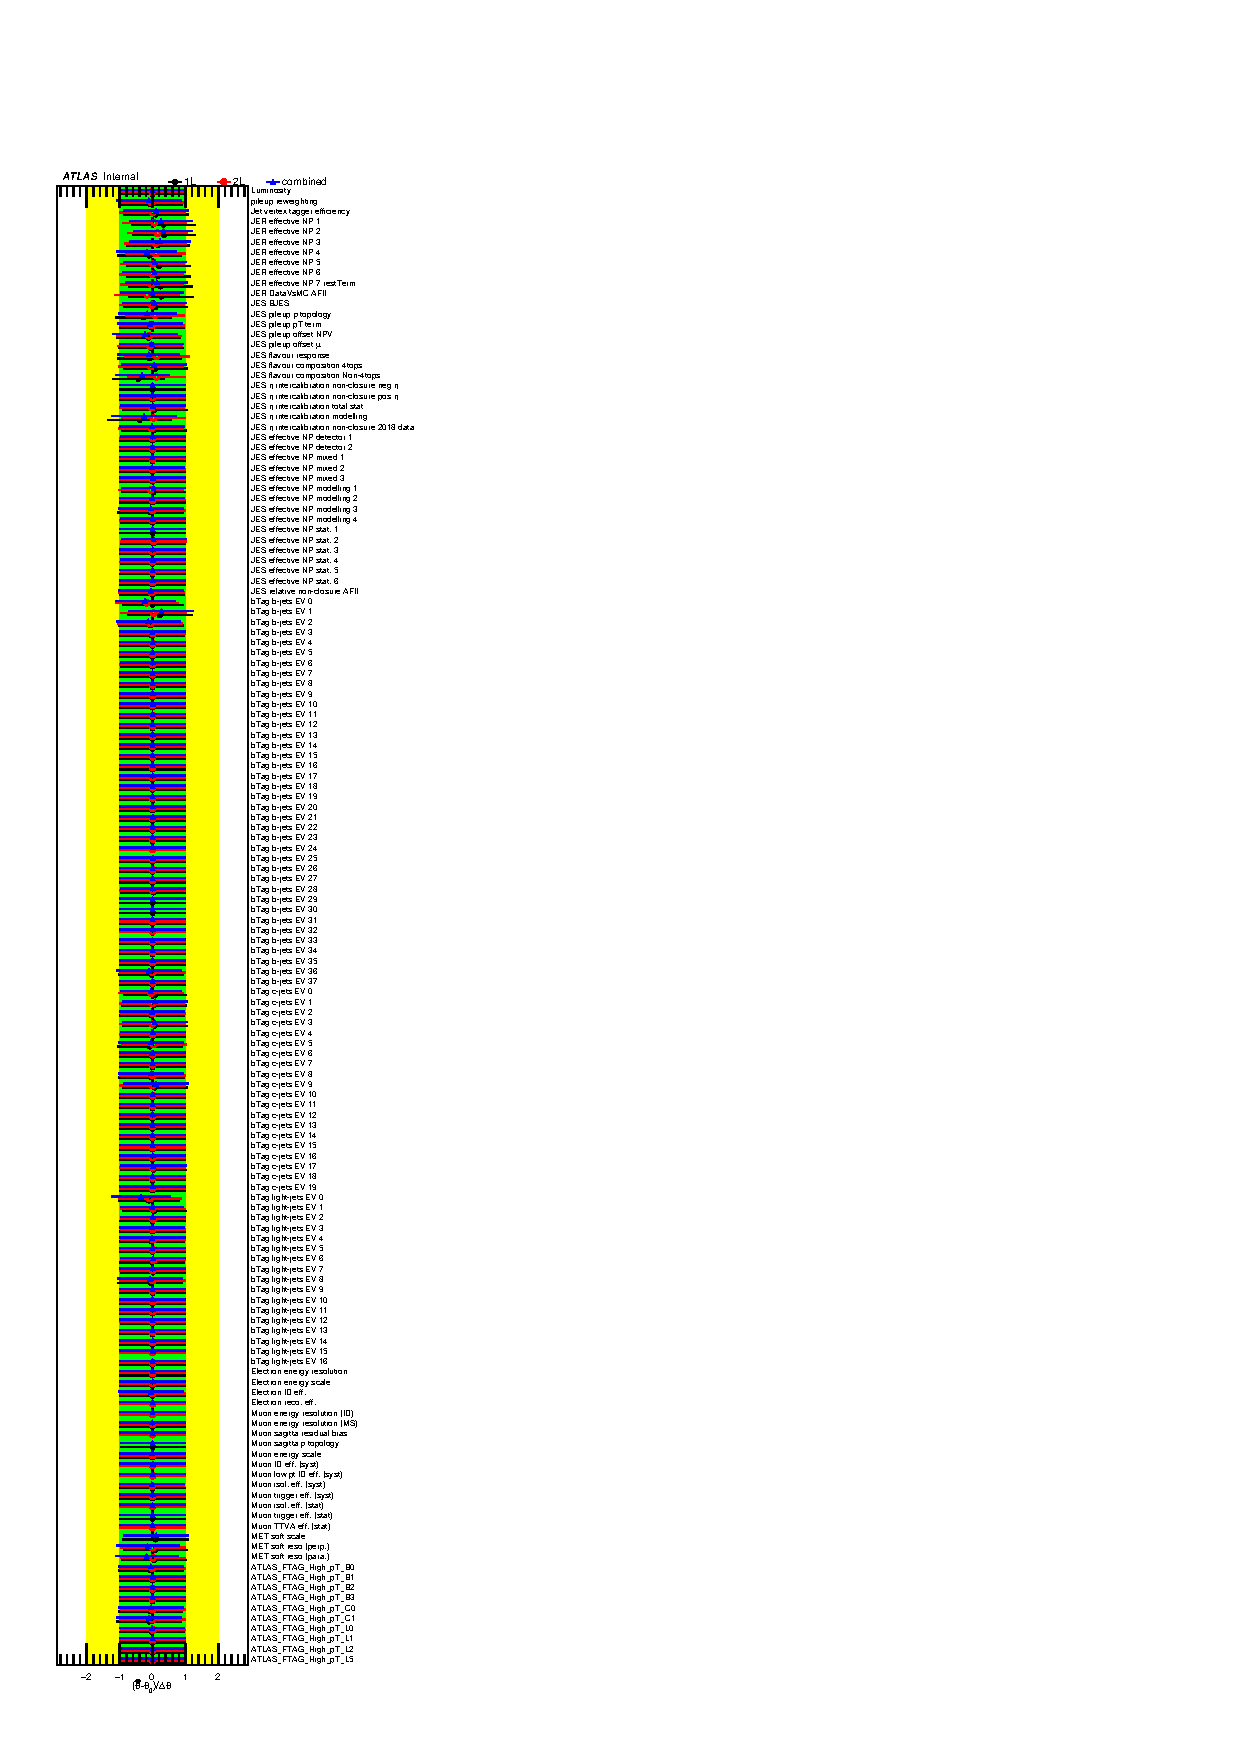
\includegraphics[width=\linewidth]{figures/fits/comparisons/selections/GNN/700/data_unblindedSplusB/NuisPar_comp_Instrumental.pdf}
    \subcaption{mH=700\gev}
    \label{fig:unblinded_data_SplusB_NP_mH400}
  \end{subfigure}
  \begin{subfigure}[t]{0.32\textwidth}
    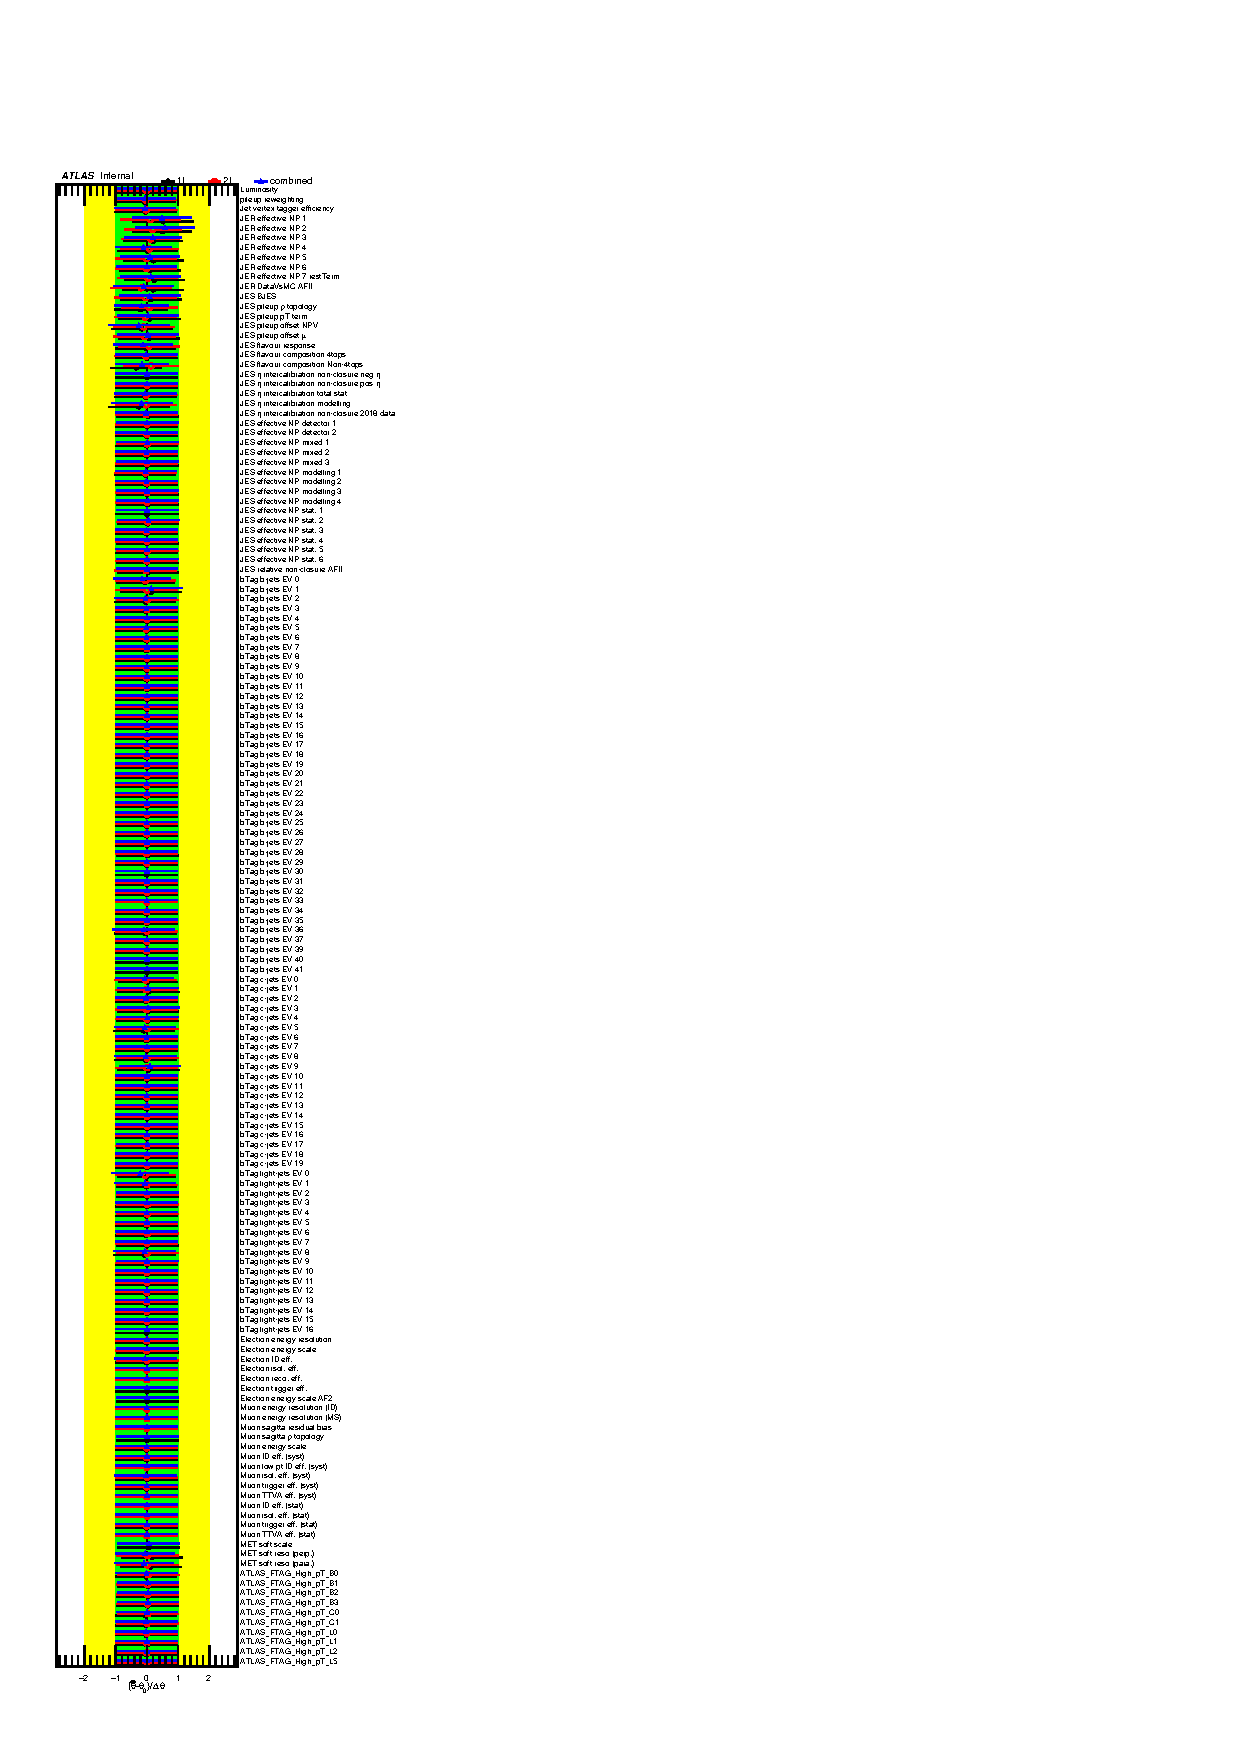
\includegraphics[width=\linewidth]{figures/fits/comparisons/selections/GNN/1000/data_unblindedSplusB/NuisPar_comp_Instrumental.pdf}
    \subcaption{mH=1000\gev}
    \label{fig:unblinded_data_SplusB_NP_mH400}
  \end{subfigure}
  \caption{\label{fig:unblinded_data_SplusB_NP_instrumental}Fitted pulls and constraints for the nuisance parameters corresponding to the instrumental systematic uncertainties for the signal+background unblinded Data fit for three mass points. Comparison is done for three fits: using only 1L regions, using only 2LOS regions and using all regions.}
\end{figure}


\begin{figure}[htbp!]
  \centering
  \begin{subfigure}[t]{0.32\textwidth}
    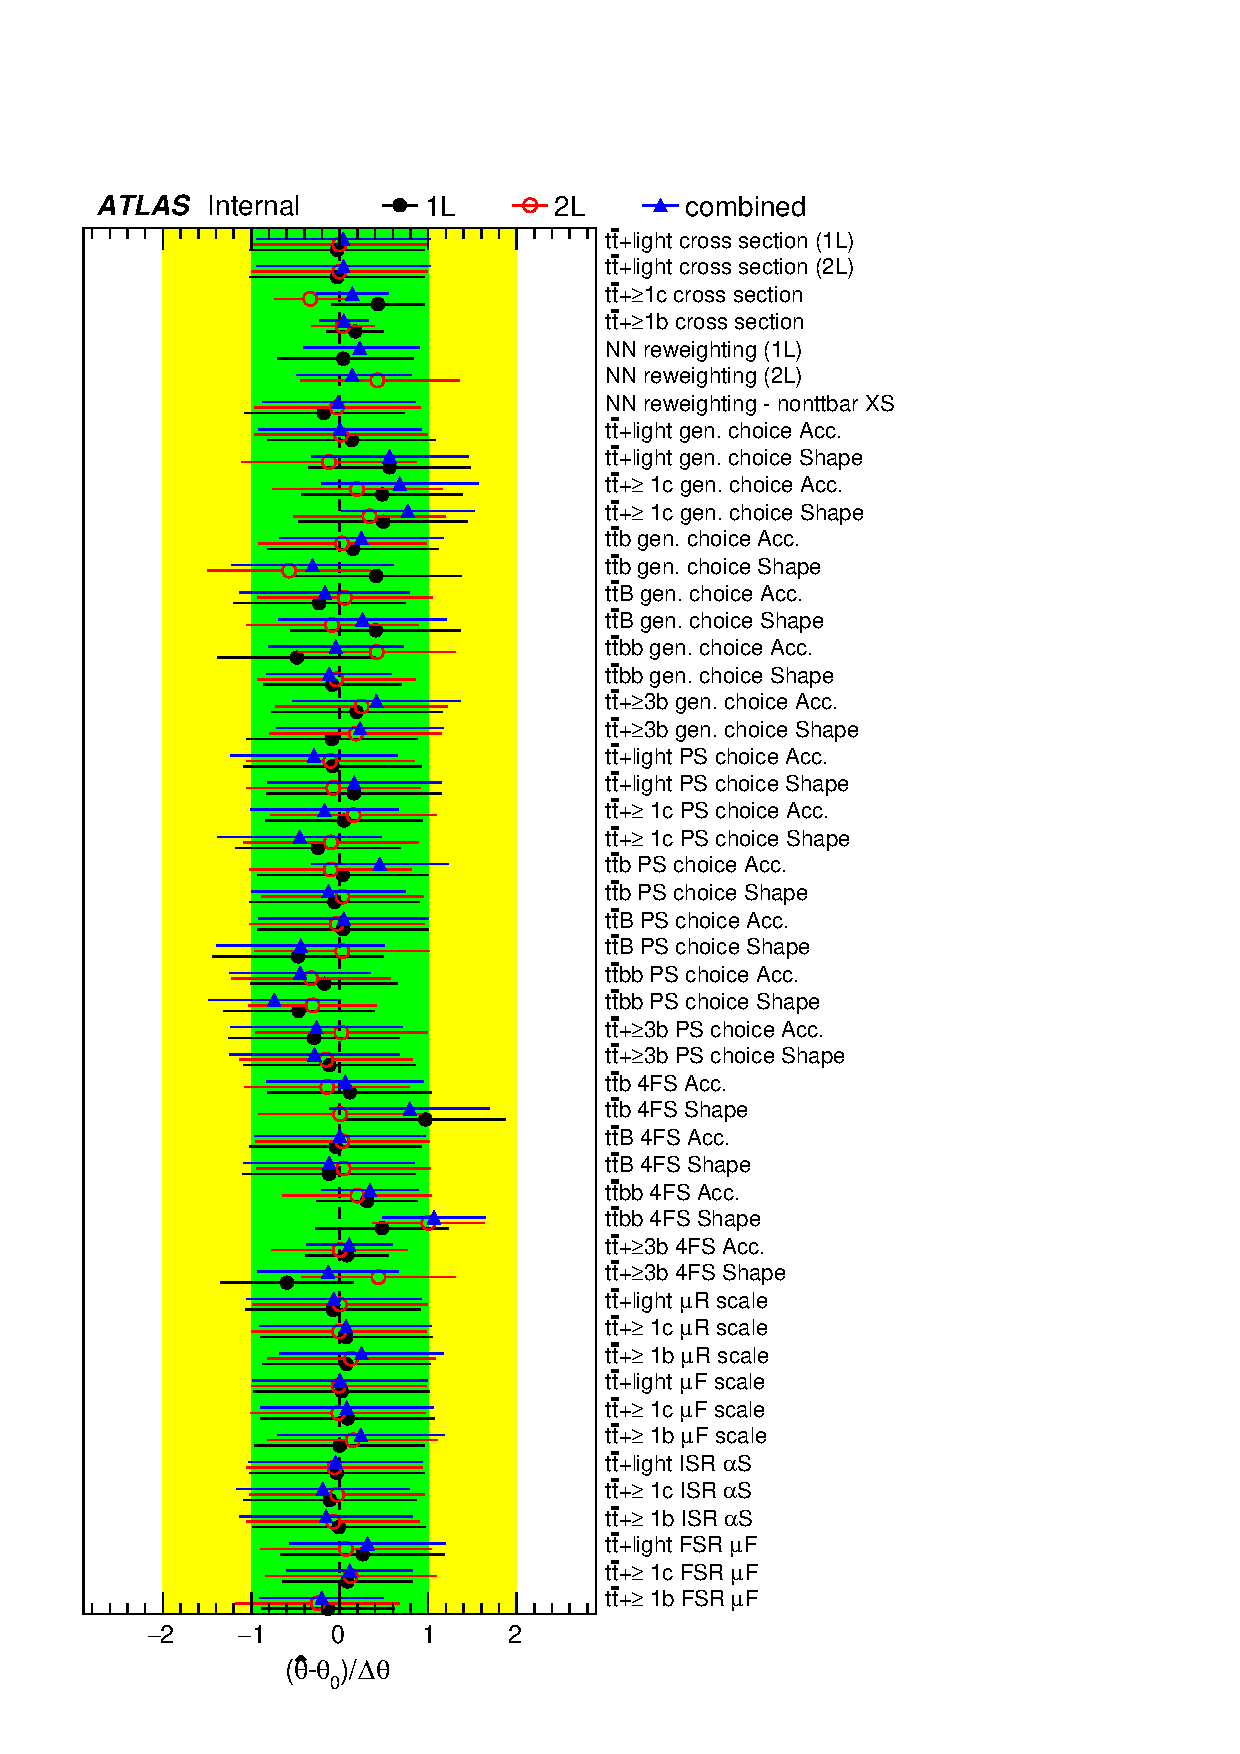
\includegraphics[width=\linewidth]{figures/fits/comparisons/selections/GNN/400/data_unblindedSplusB/NuisPar_comp_ttbar.pdf}
    \subcaption{mH=400\gev}
    \label{fig:unblinded_data_SplusB_NP_mH400}
  \end{subfigure}
  \begin{subfigure}[t]{0.32\textwidth}
    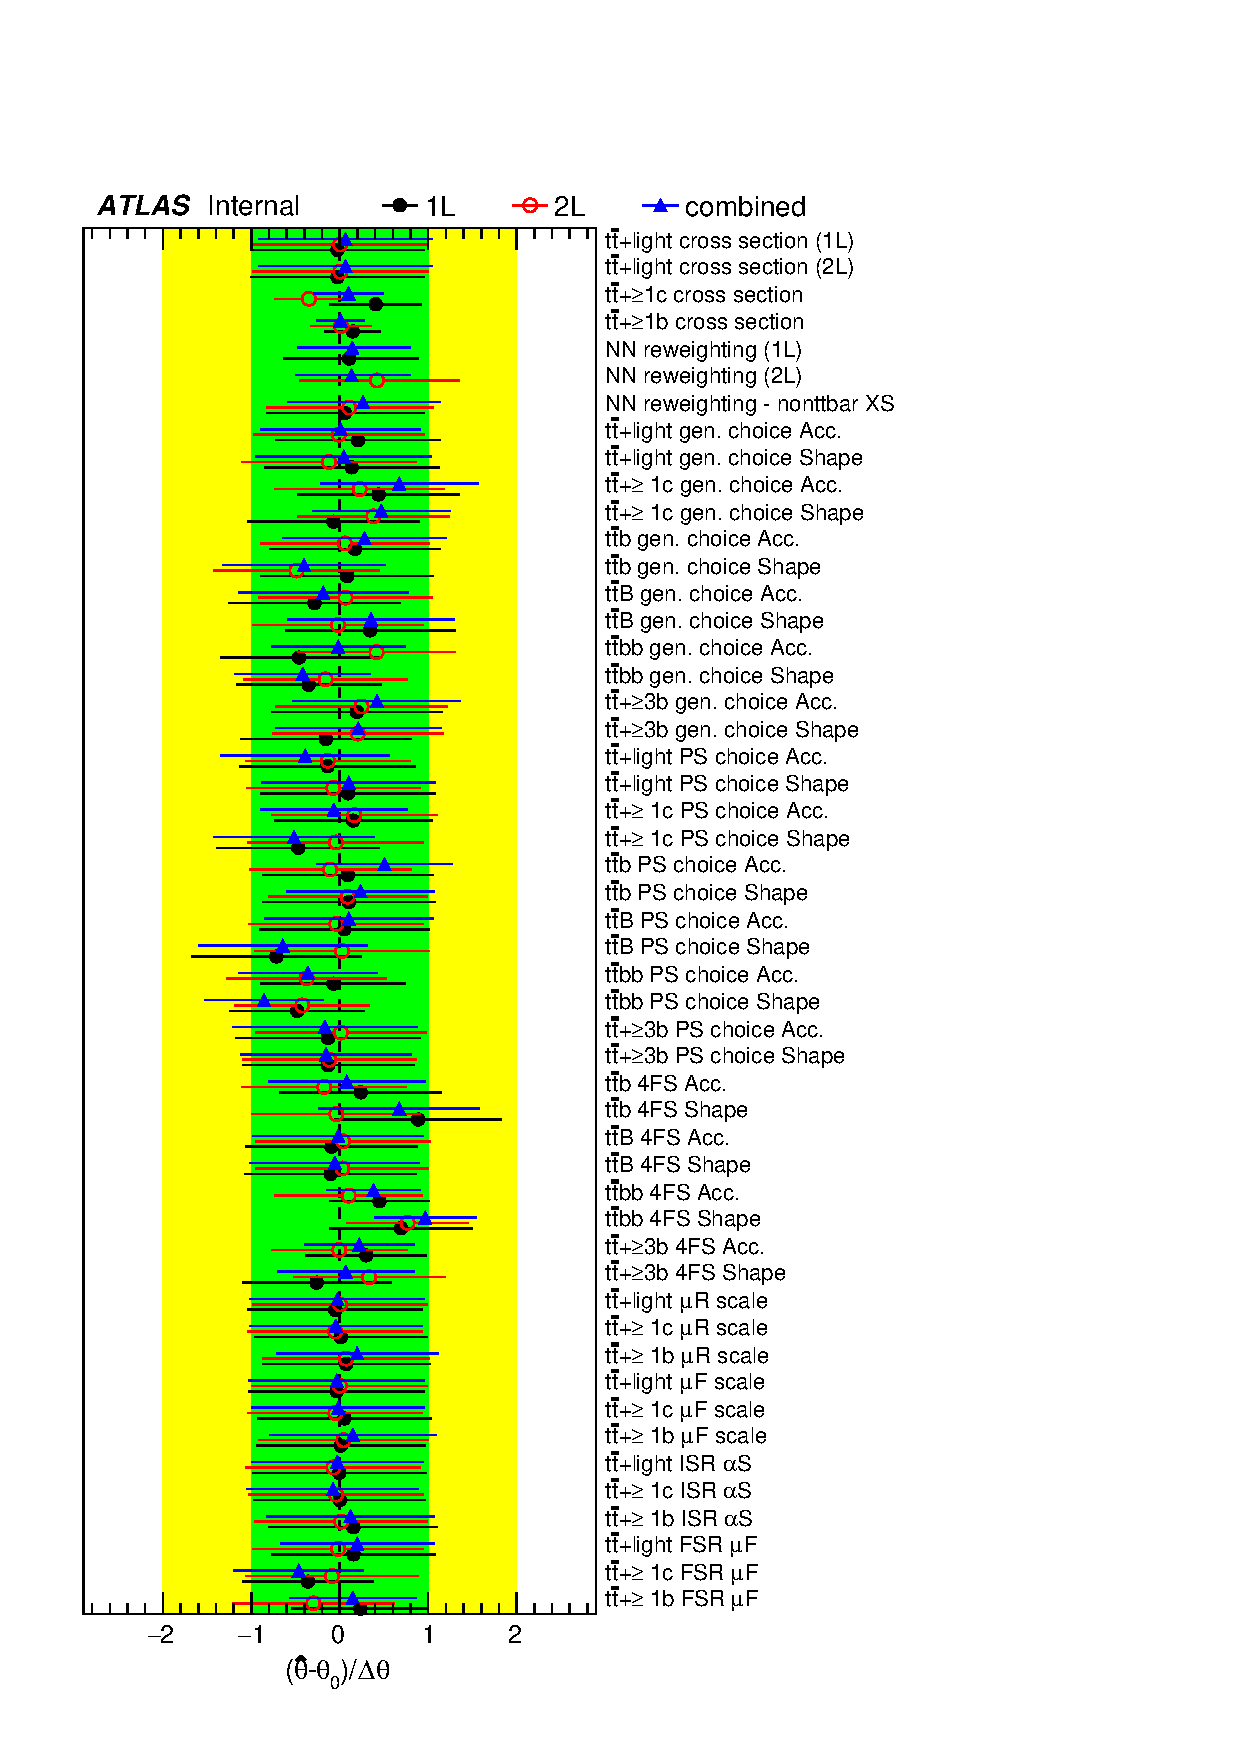
\includegraphics[width=\linewidth]{figures/fits/comparisons/selections/GNN/700/data_unblindedSplusB/NuisPar_comp_ttbar.pdf}
    \subcaption{mH=700\gev}
    \label{fig:unblinded_data_SplusB_NP_mH400}
  \end{subfigure}
  \begin{subfigure}[t]{0.32\textwidth}
    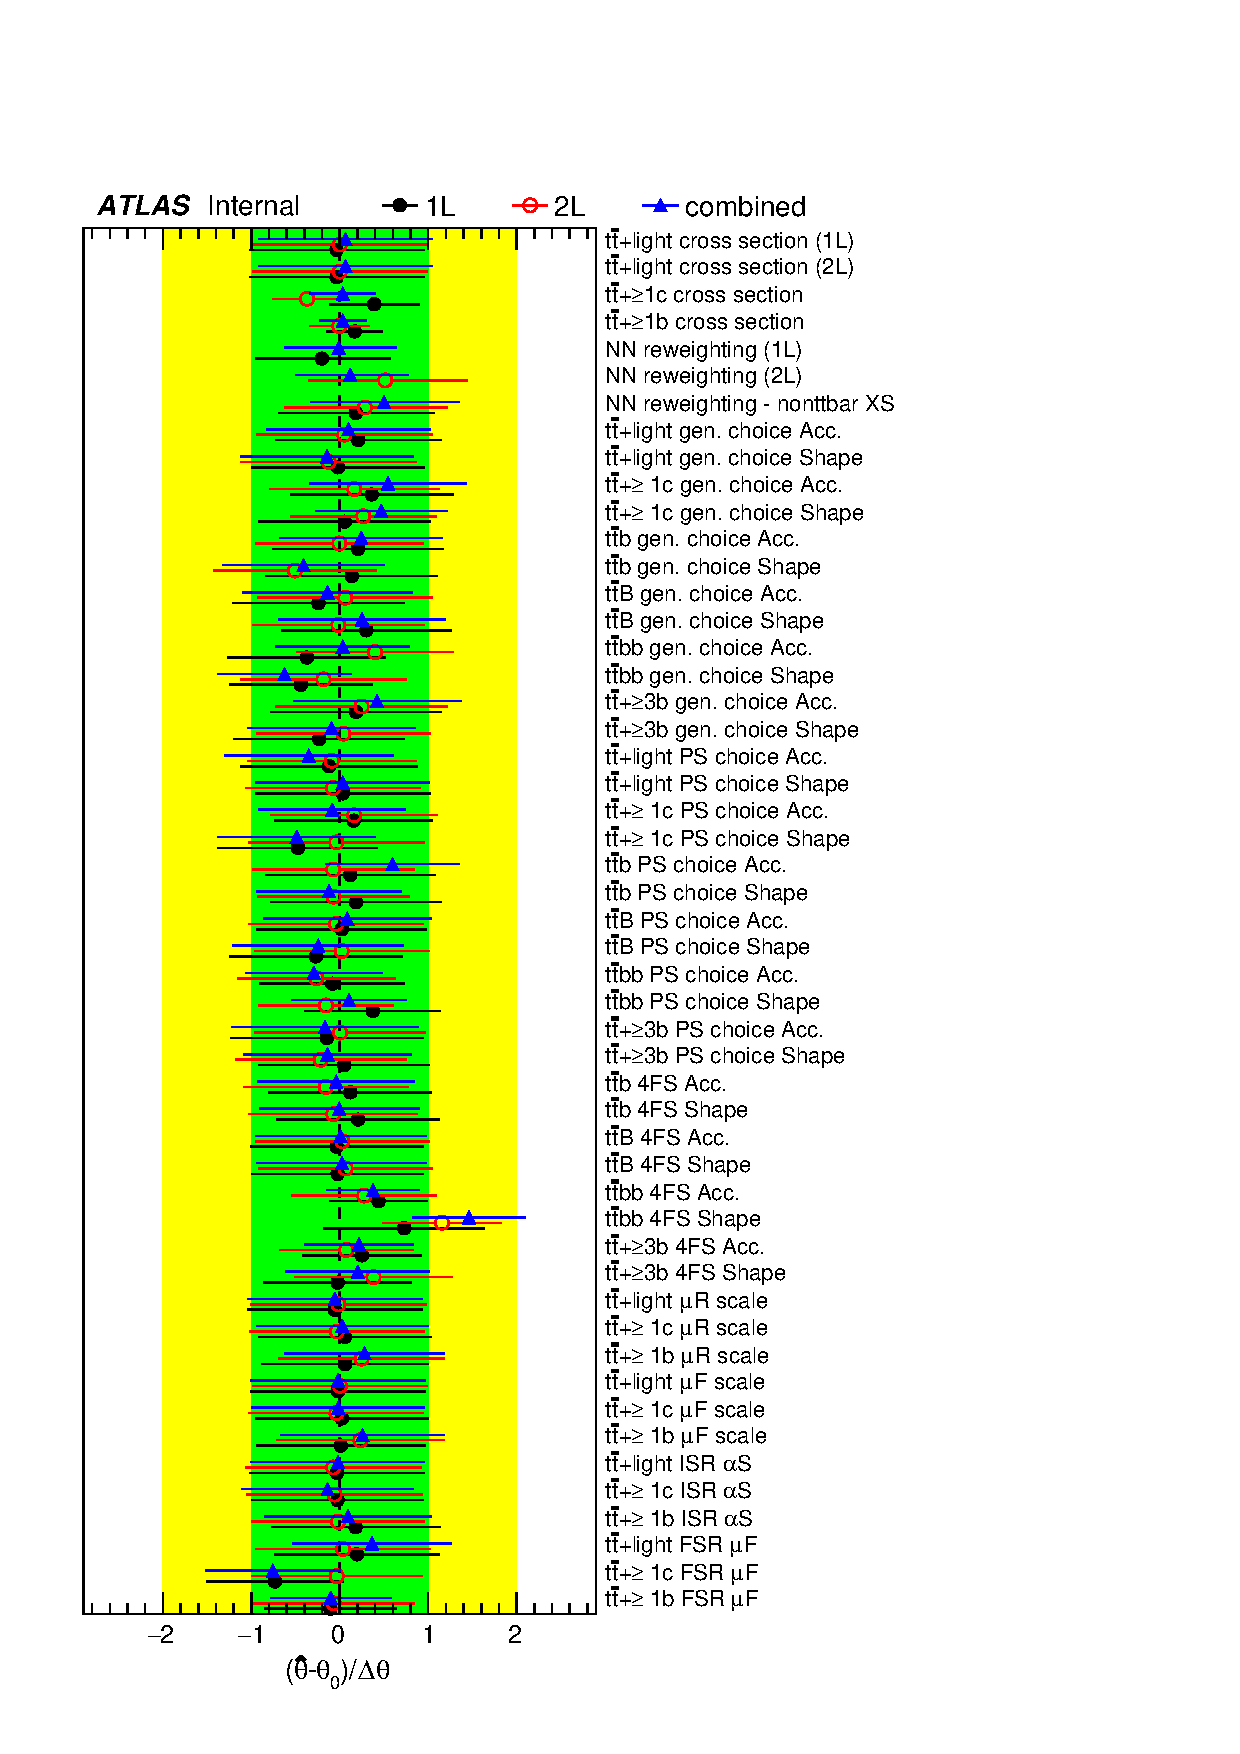
\includegraphics[width=\linewidth]{figures/fits/comparisons/selections/GNN/1000/data_unblindedSplusB/NuisPar_comp_ttbar.pdf}
    \subcaption{mH=1000\gev}
    \label{fig:unblinded_data_SplusB_NP_mH400}
  \end{subfigure}
  \caption{\label{fig:unblinded_data_SplusB_NP_ttbar}Fitted pulls and constraints for the nuisance parameters corresponding to the \ttbar systematic uncertainties for the signal+background unblinded Data fit for three mass points. Comparison is done for three fits: using only 1L regions, using only 2LOS regions and using all regions.}
\end{figure}


\begin{figure}[htbp!]
  \centering
  \begin{subfigure}[t]{0.32\textwidth}
    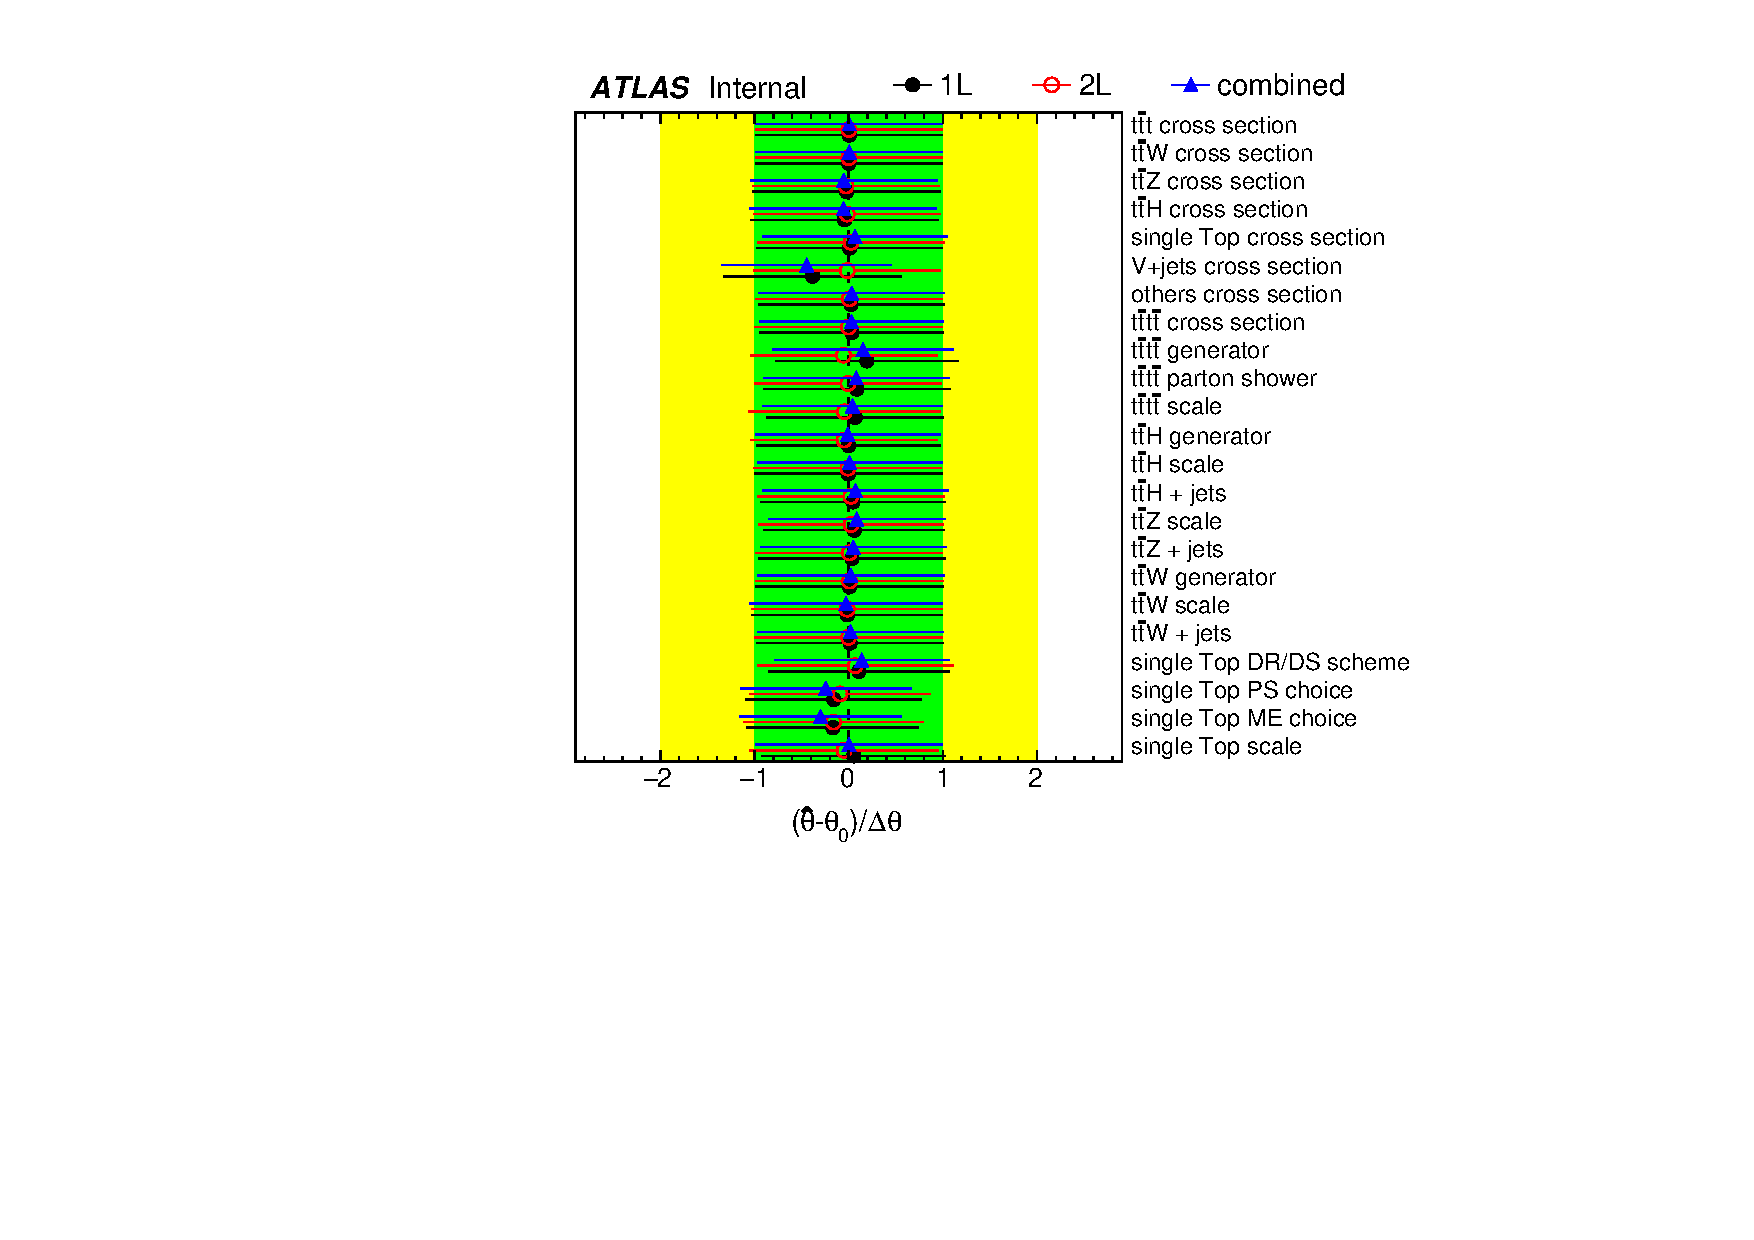
\includegraphics[width=\linewidth]{figures/fits/comparisons/selections/GNN/400/data_unblindedSplusB/NuisPar_comp_Other.pdf}
    \subcaption{mH=400\gev}
    \label{fig:unblinded_data_SplusB_NP_mH400}
  \end{subfigure}
  \begin{subfigure}[t]{0.32\textwidth}
    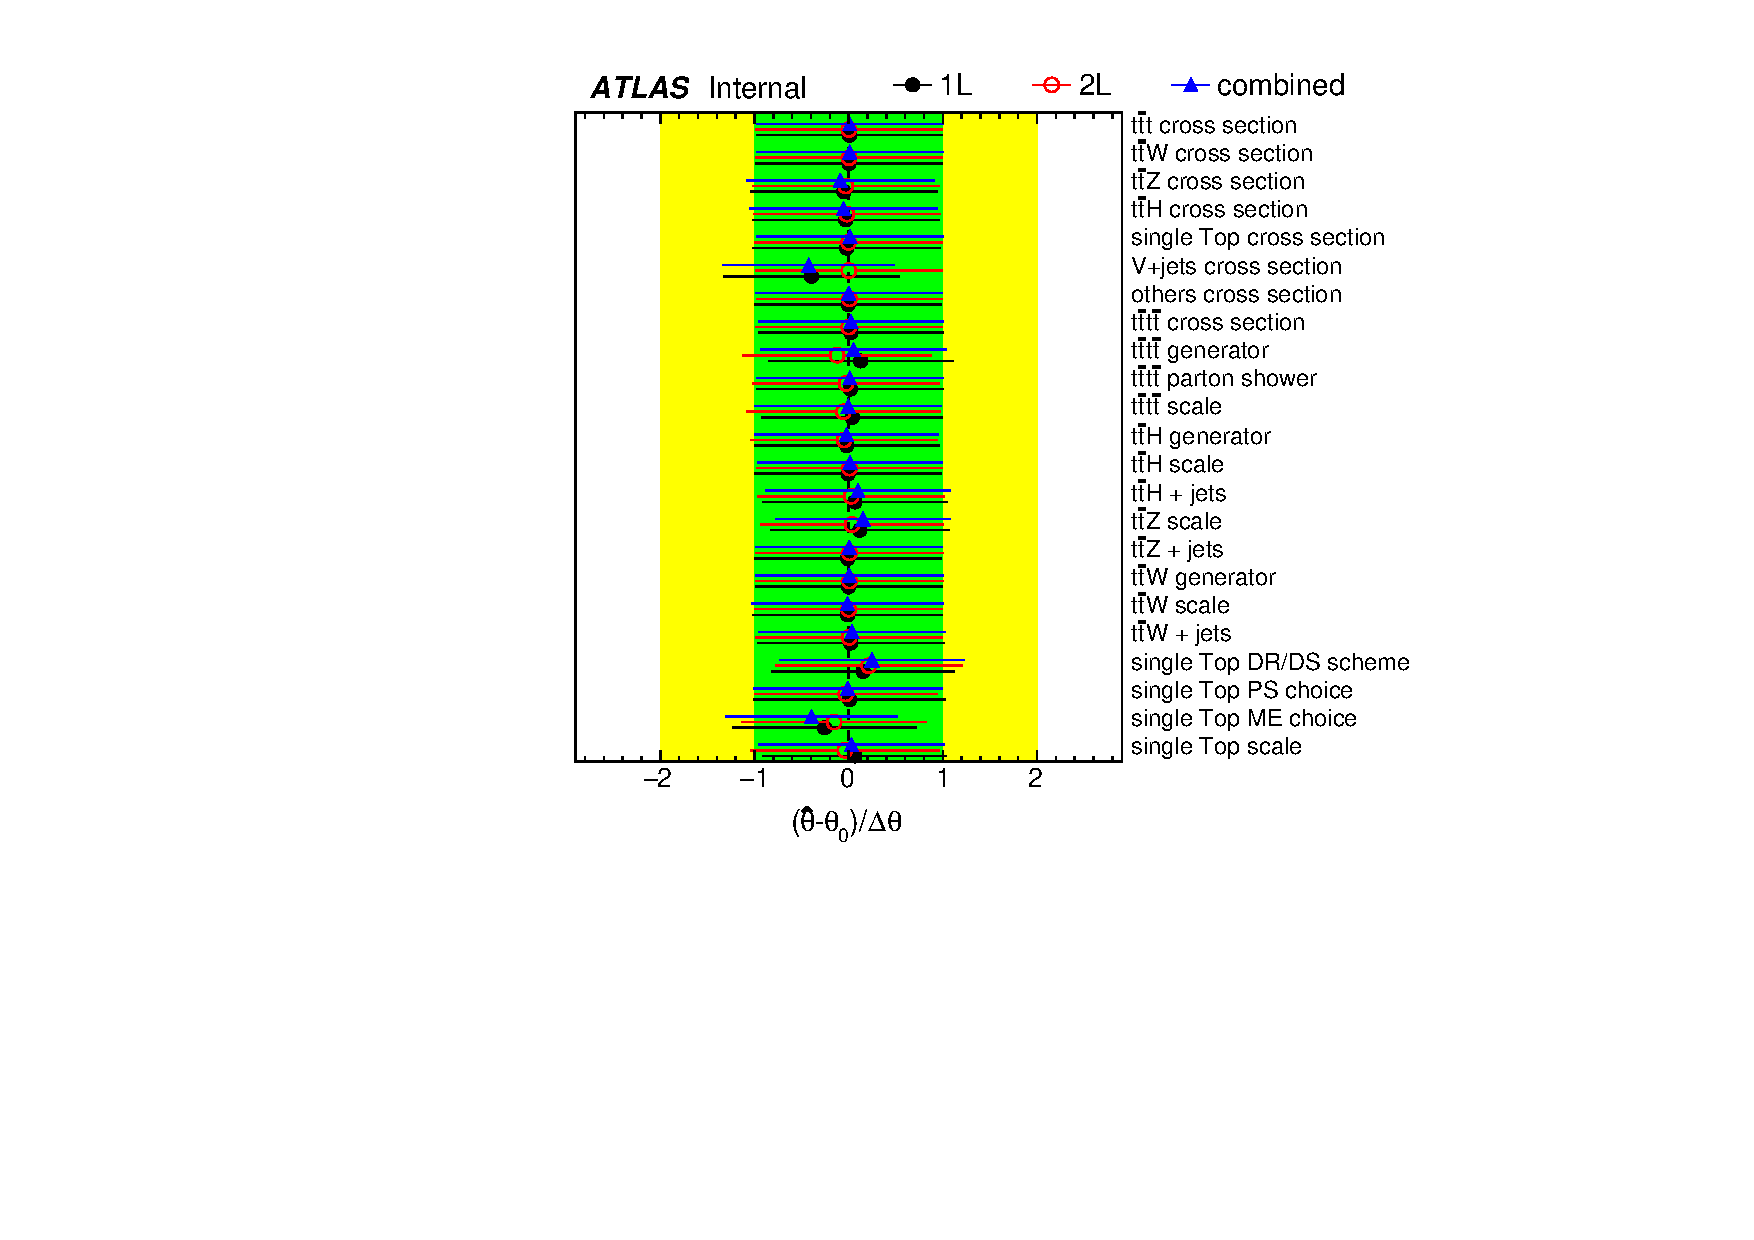
\includegraphics[width=\linewidth]{figures/fits/comparisons/selections/GNN/700/data_unblindedSplusB/NuisPar_comp_Other.pdf}
    \subcaption{mH=700\gev}
    \label{fig:unblinded_data_SplusB_NP_mH400}
  \end{subfigure}
  \begin{subfigure}[t]{0.32\textwidth}
    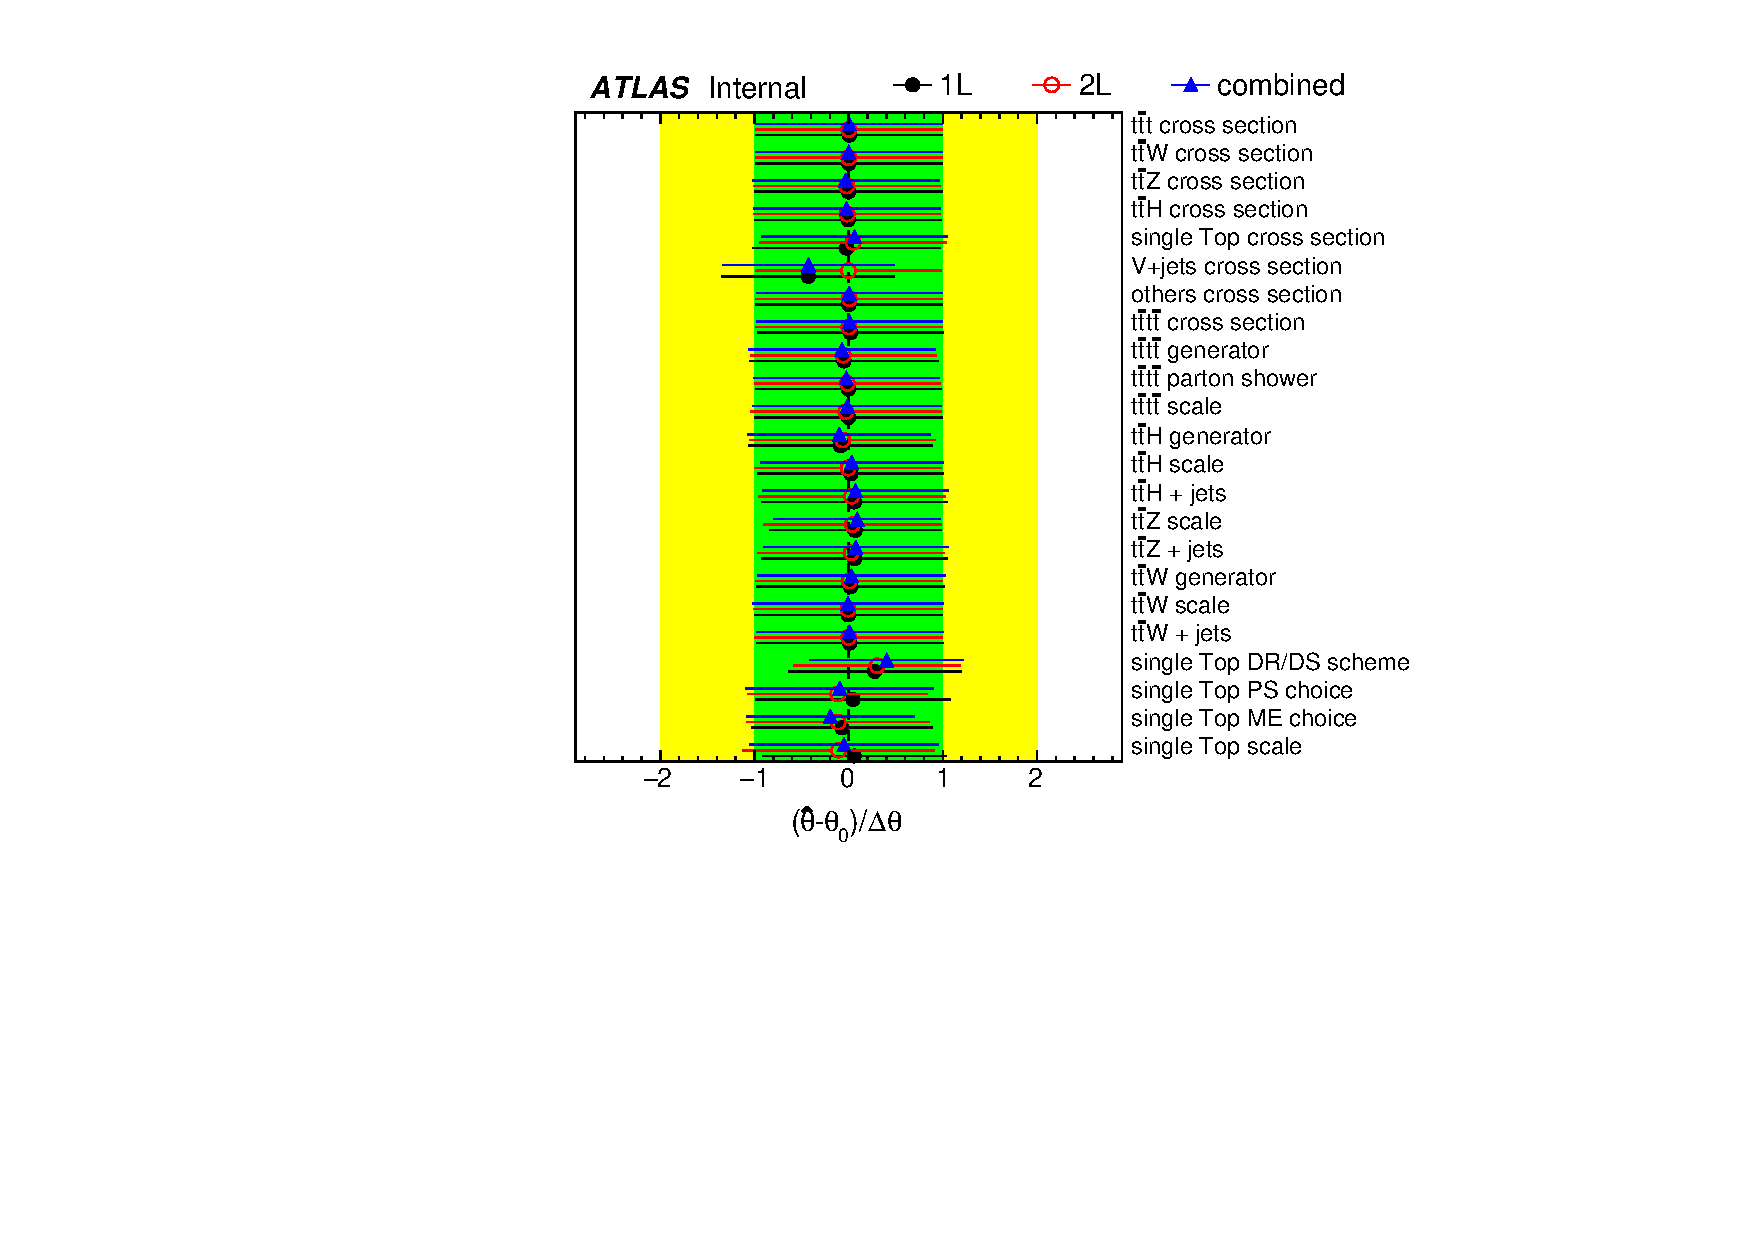
\includegraphics[width=\linewidth]{figures/fits/comparisons/selections/GNN/1000/data_unblindedSplusB/NuisPar_comp_Other.pdf}
    \subcaption{mH=1000\gev}
    \label{fig:unblinded_data_SplusB_NP_mH400}
  \end{subfigure}
  \caption{\label{fig:unblinded_data_SplusB_NP_other}Fitted pulls and constraints for the  nuisance parameters corresponding to the non-\ttbar-background systematic uncertainties for the signal+background unblinded Data fit for three mass points. Comparison is done for three fits: using only 1L regions, using only 2LOS regions and using all regions.}
\end{figure}



\begin{figure}[htbp!]
  \centering
  \begin{subfigure}[t]{0.32\textwidth}
    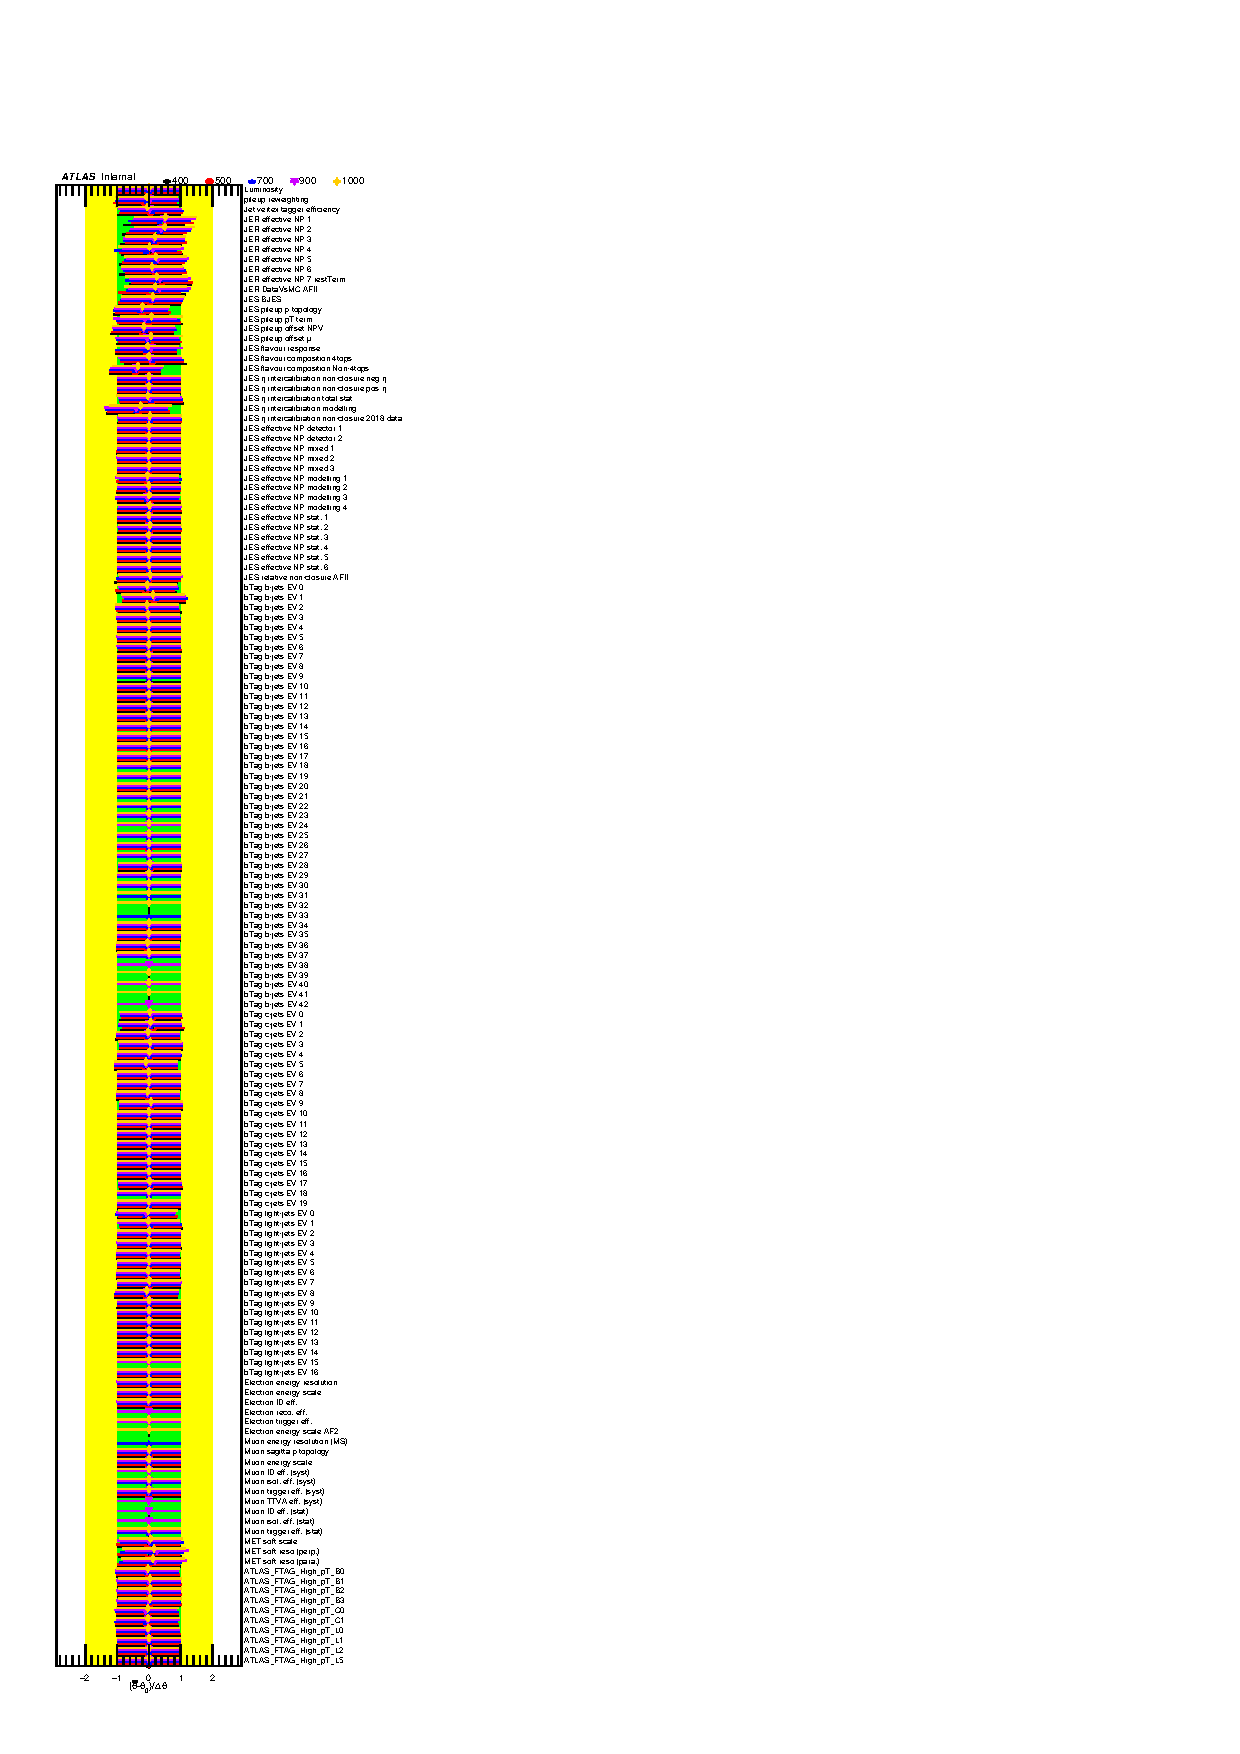
\includegraphics[width=\linewidth]{figures/fits/comparisons/massPoints/GNN/1L/data_unblindedSplusB/NuisPar_comp_Instrumental.pdf}
    \subcaption{1L}
    \label{fig:unblinded_data_SplusB_NP_1L_instrumental}
  \end{subfigure}
  \begin{subfigure}[t]{0.32\textwidth}
    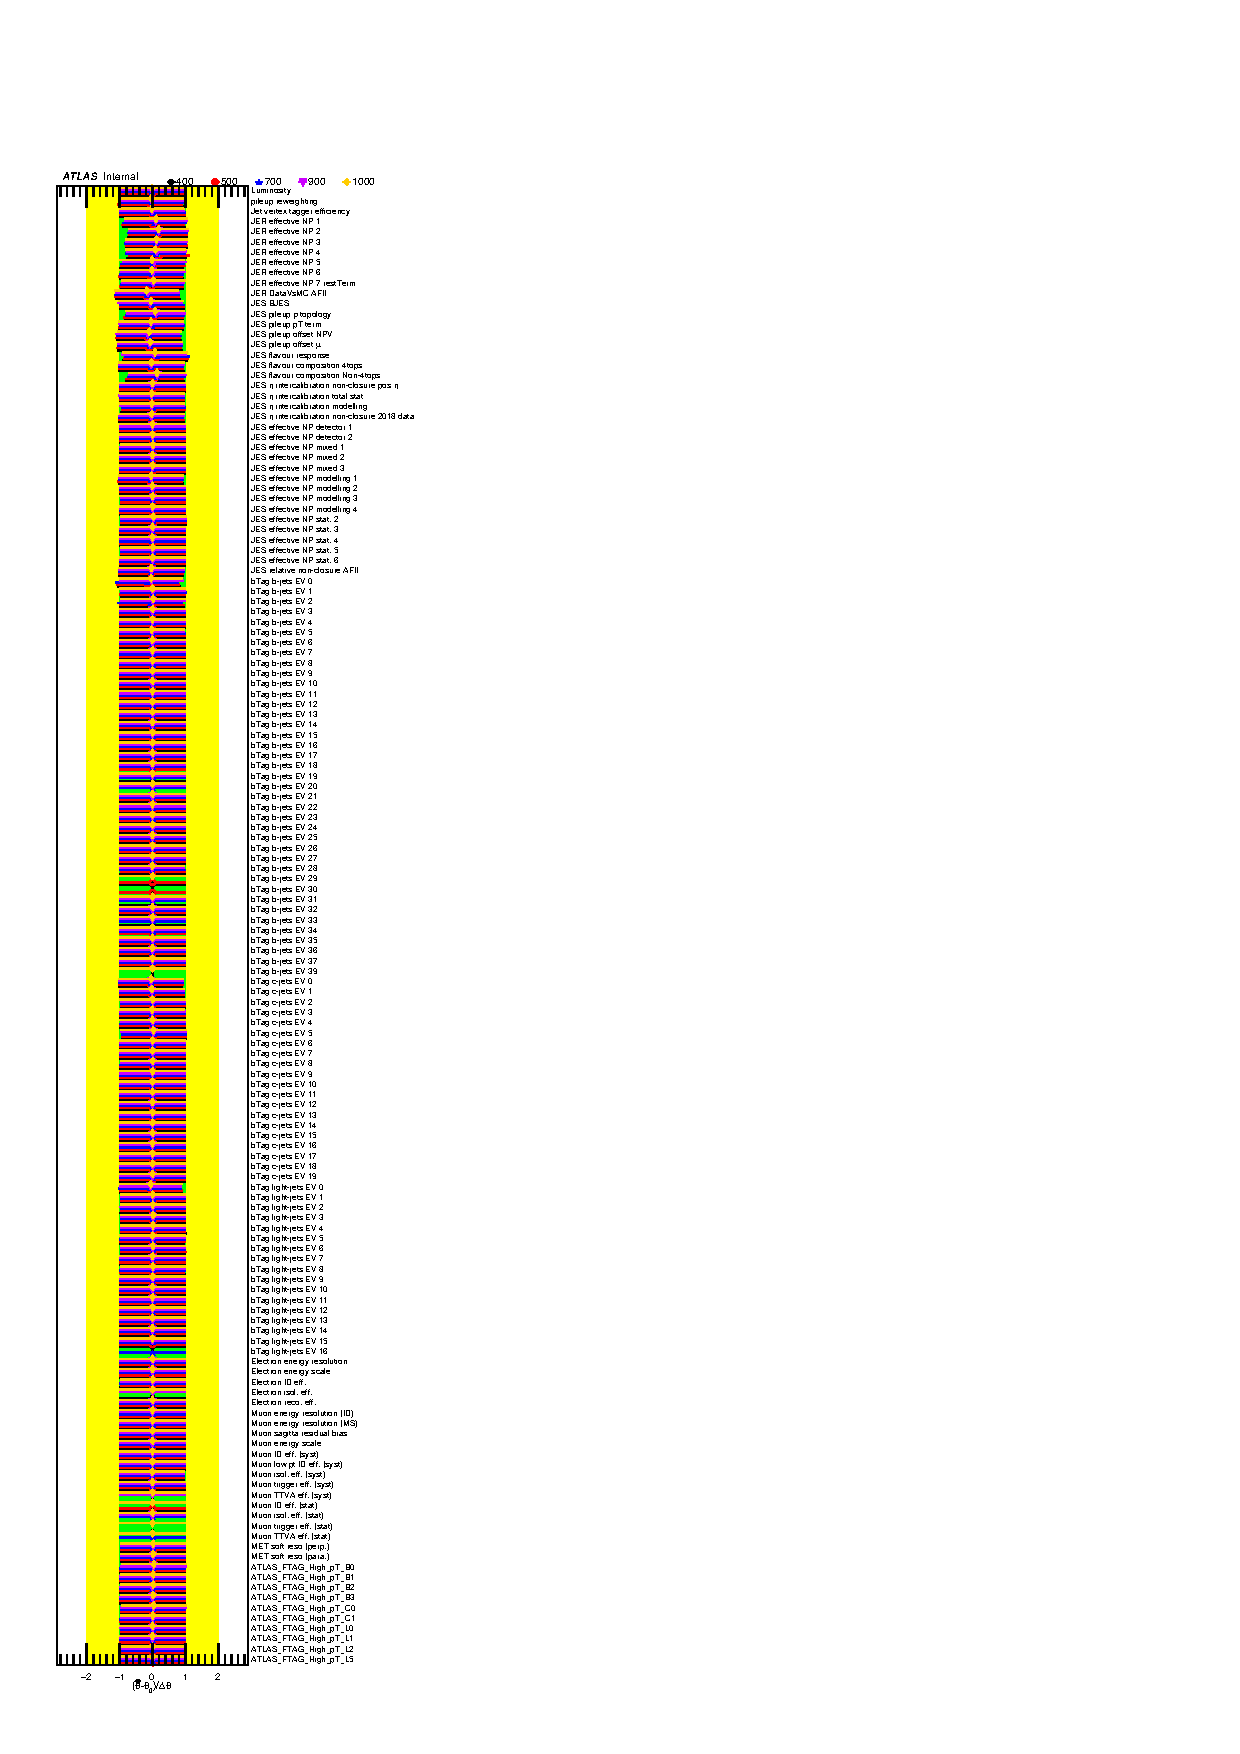
\includegraphics[width=\linewidth]{figures/fits/comparisons/massPoints/GNN/2L/data_unblindedSplusB/NuisPar_comp_Instrumental.pdf}
    \subcaption{2L}
    \label{fig:unblinded_data_SplusB_NP_2L_instrumental}
  \end{subfigure}
  \begin{subfigure}[t]{0.32\textwidth}
    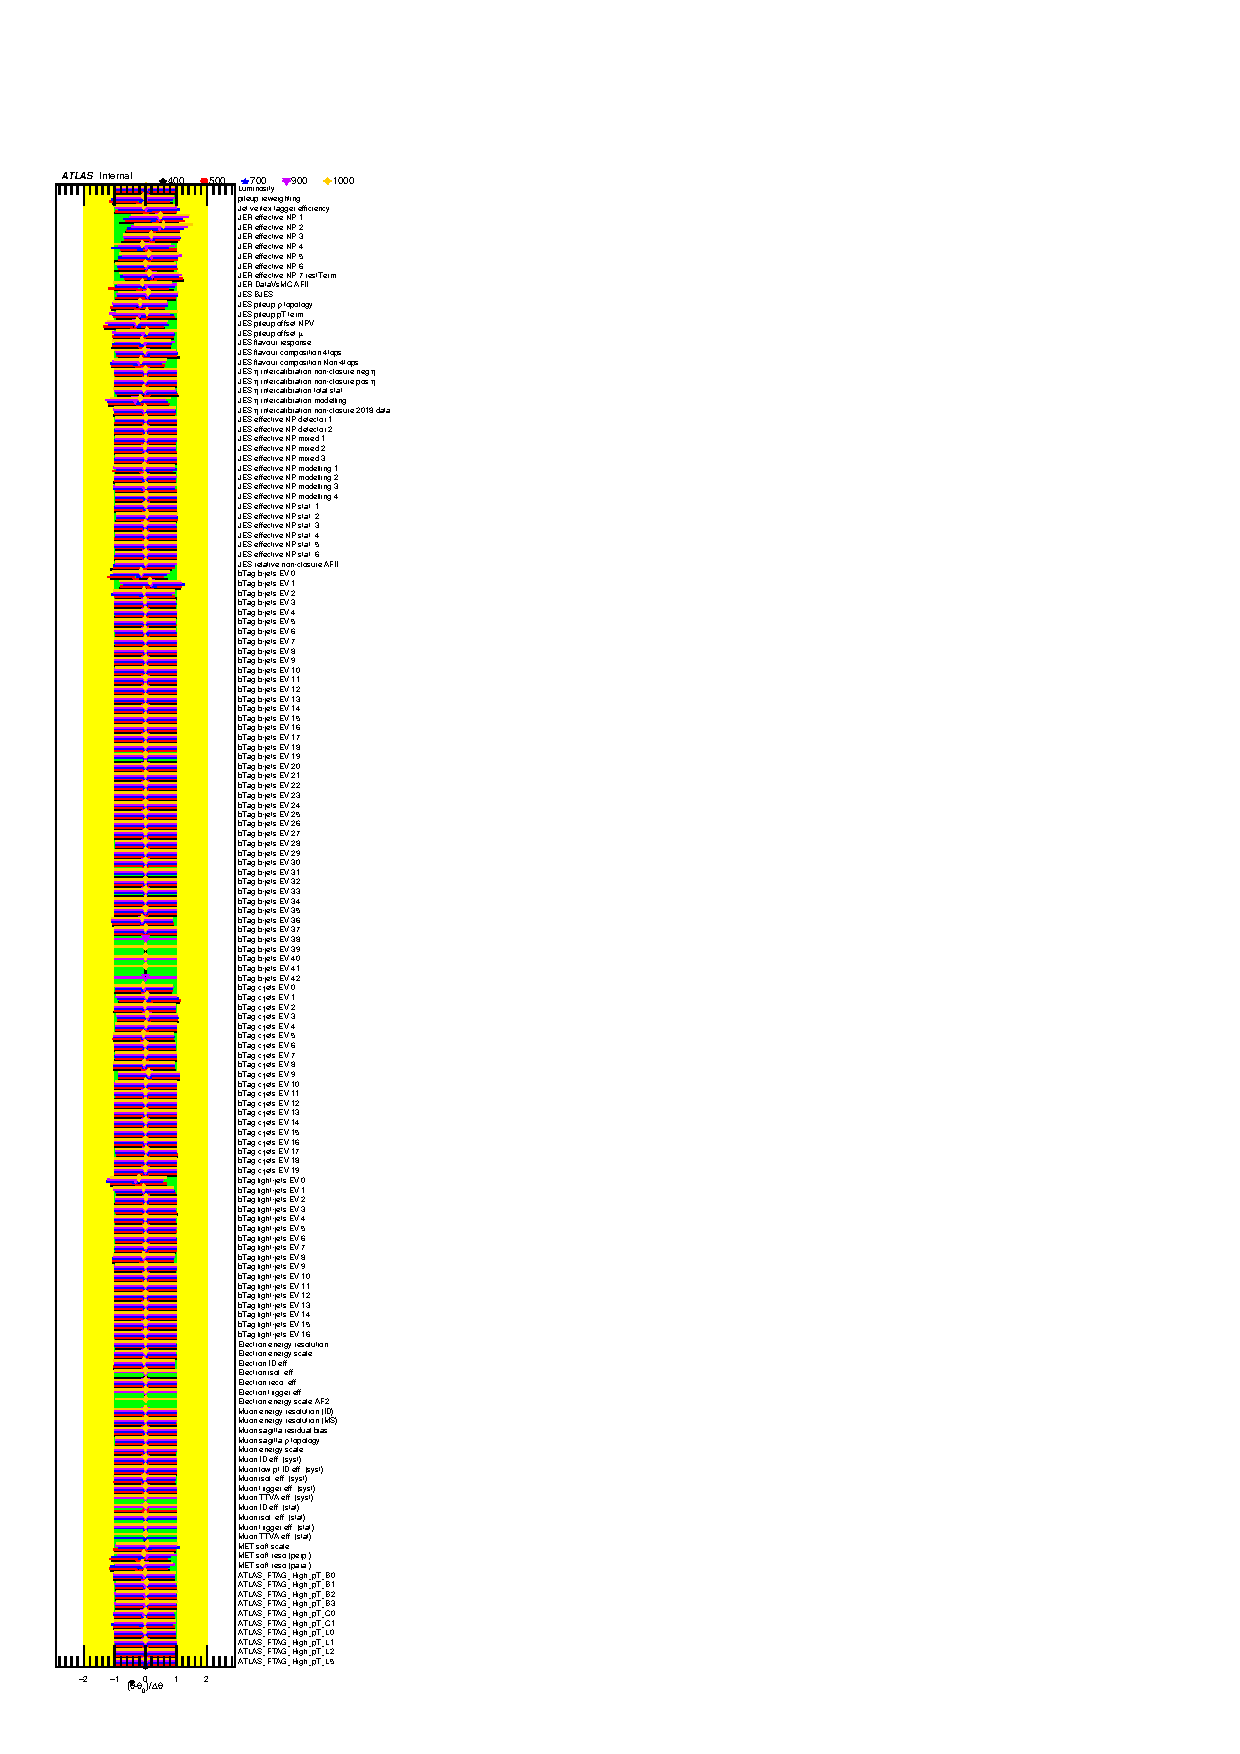
\includegraphics[width=\linewidth]{figures/fits/comparisons/massPoints/GNN/all/data_unblindedSplusB/NuisPar_comp_Instrumental.pdf}
    \subcaption{1L+2L}
    \label{fig:unblinded_data_SplusB_NP_all_instrumental}
  \end{subfigure}
  \caption{Fitted pulls and constraints for the nuisance parameters corresponding to the instrumental systematic uncertainties for the signal+background unblinded Data fit for three types of fits: using only 1L regions, using only 2L regions, and using all regions. Comparison is done for five mass points.}
\label{fig:unblinded_data_SplusB_NP_mass_instrumental}
\end{figure}


\begin{figure}[htbp!]
  \centering
  \begin{subfigure}[t]{0.32\textwidth}
    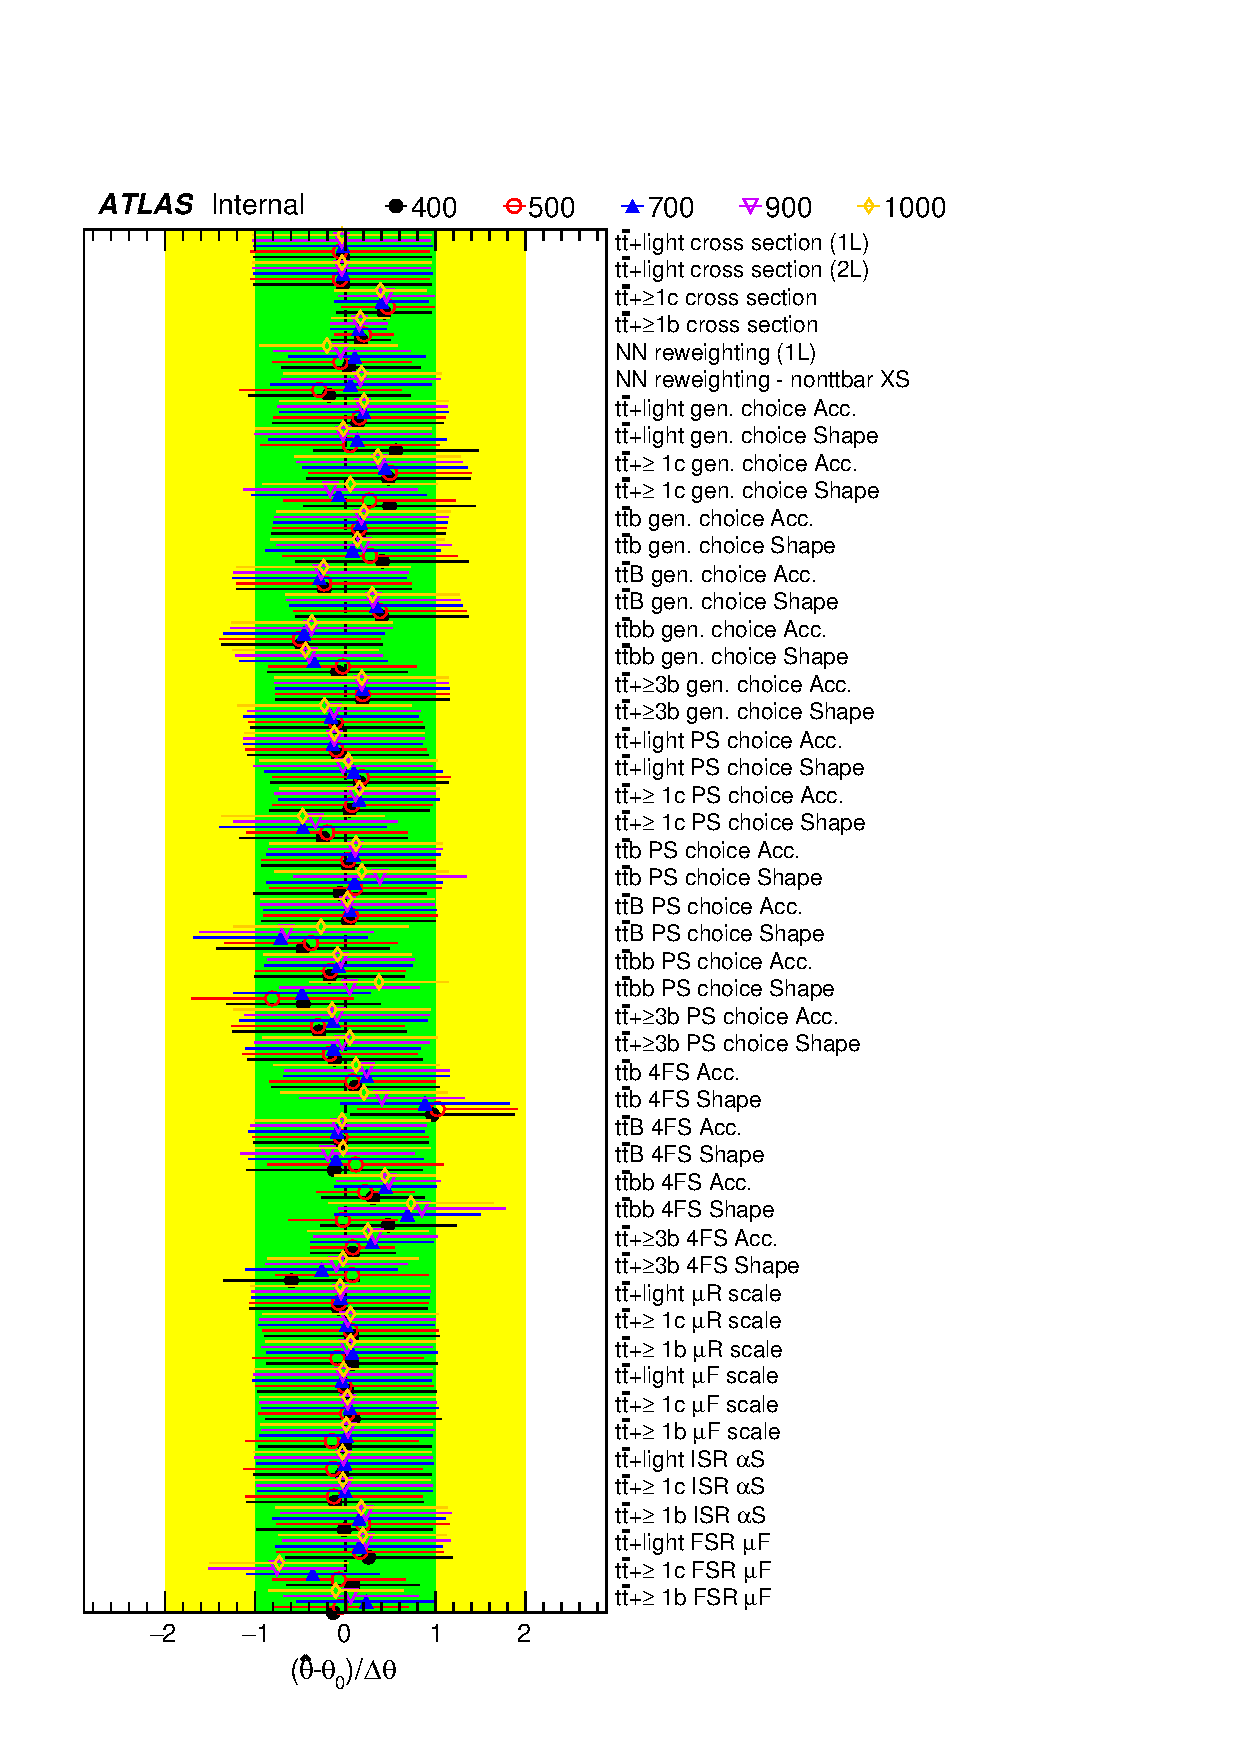
\includegraphics[width=\linewidth]{figures/fits/comparisons/massPoints/GNN/1L/data_unblindedSplusB/NuisPar_comp_ttbar.pdf}
    \subcaption{1L}
    \label{fig:unblinded_data_SplusB_NP_1L}
  \end{subfigure}
  \begin{subfigure}[t]{0.32\textwidth}
    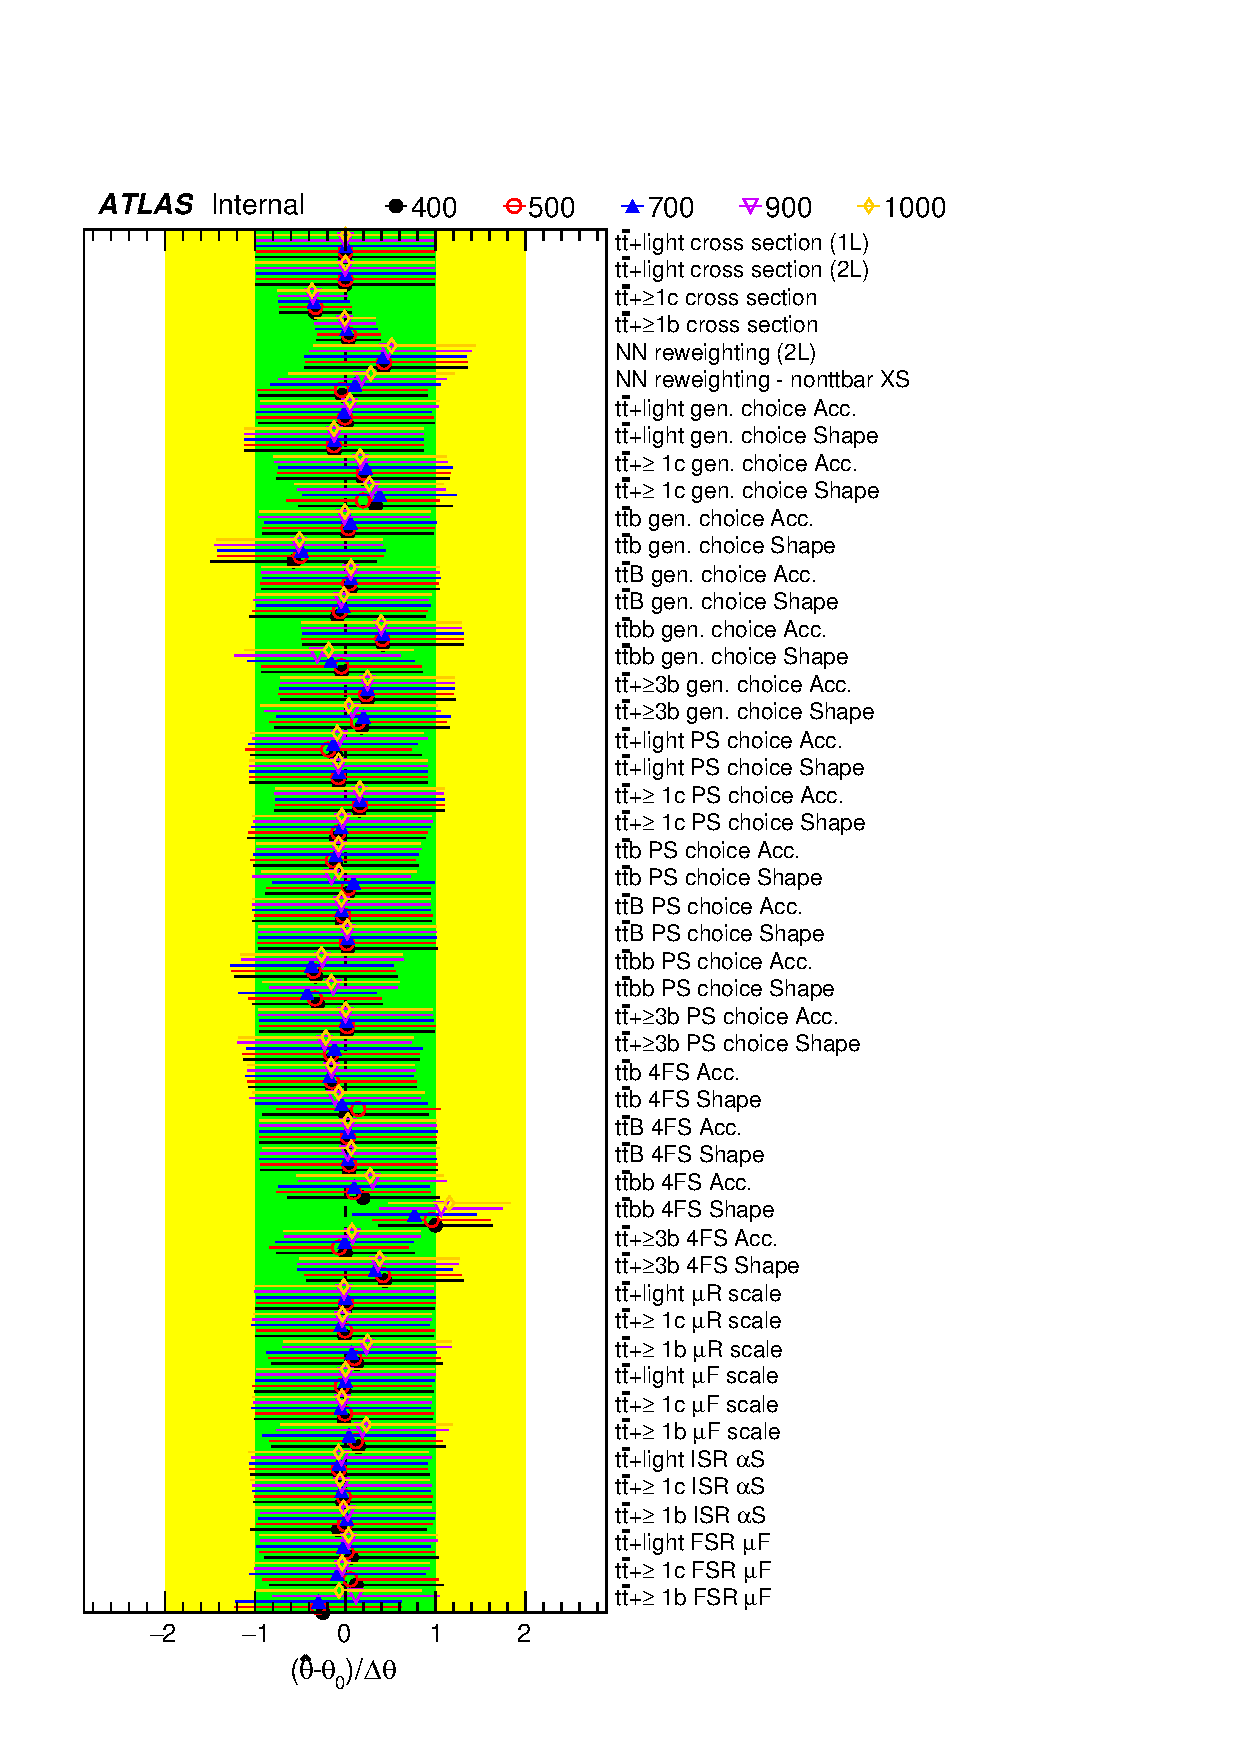
\includegraphics[width=\linewidth]{figures/fits/comparisons/massPoints/GNN/2L/data_unblindedSplusB/NuisPar_comp_ttbar.pdf}
    \subcaption{2L}
    \label{fig:unblinded_data_SplusB_NP_2L}
  \end{subfigure}
  \begin{subfigure}[t]{0.32\textwidth}
    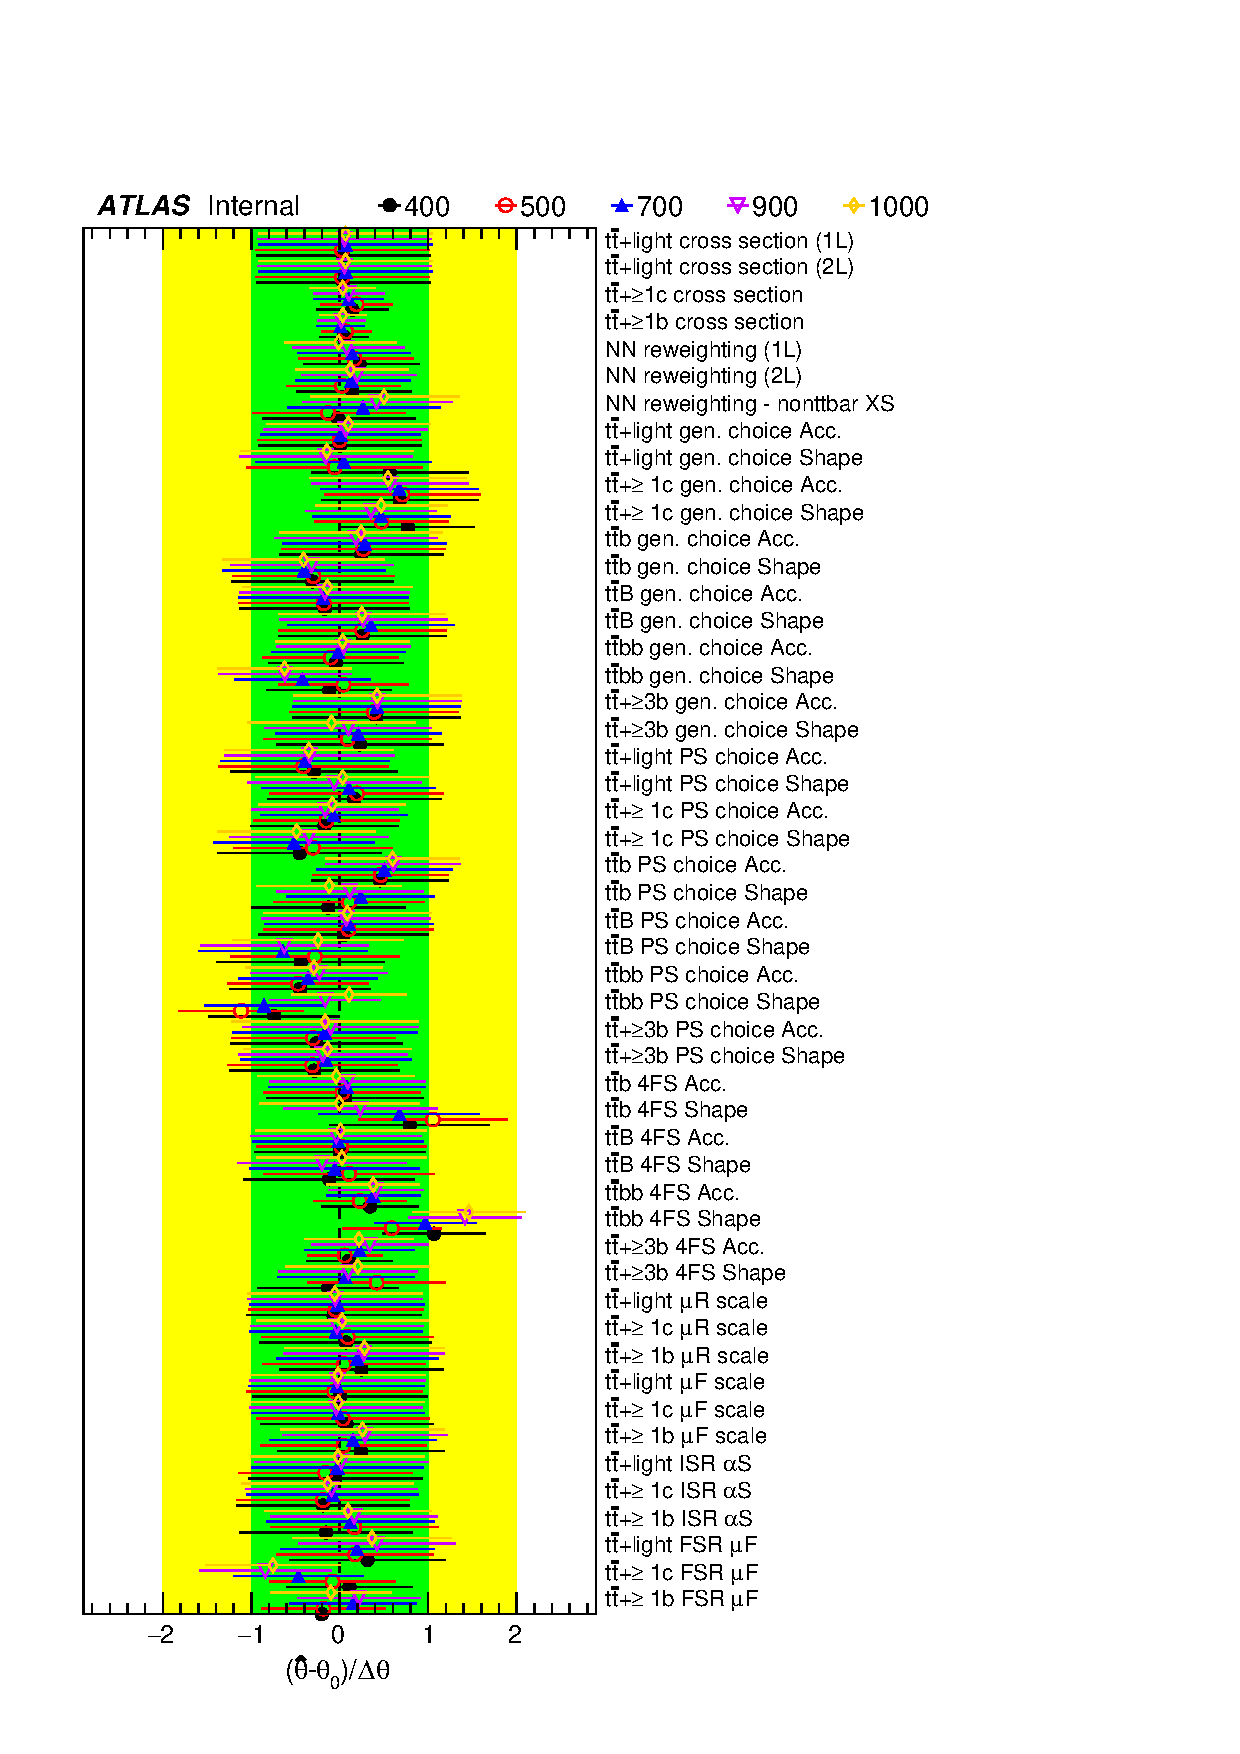
\includegraphics[width=\linewidth]{figures/fits/comparisons/massPoints/GNN/all/data_unblindedSplusB/NuisPar_comp_ttbar.pdf}
    \subcaption{1L+2L}
    \label{fig:unblinded_data_SplusB_NP_all}
  \end{subfigure}
  \caption{Fitted pulls and constraints for the nuisance parameters corresponding to the \ttbar systematic uncertainties for the signal+background unblinded Data fit for three types of fits: using only 1L regions, using only 2L regions, and using all regions. Comparison is done for five mass points.}
\label{fig:unblinded_data_SplusB_NP_mass_ttbar}
\end{figure}


\begin{figure}[htbp!]
  \centering
  \begin{subfigure}[t]{0.32\textwidth}
    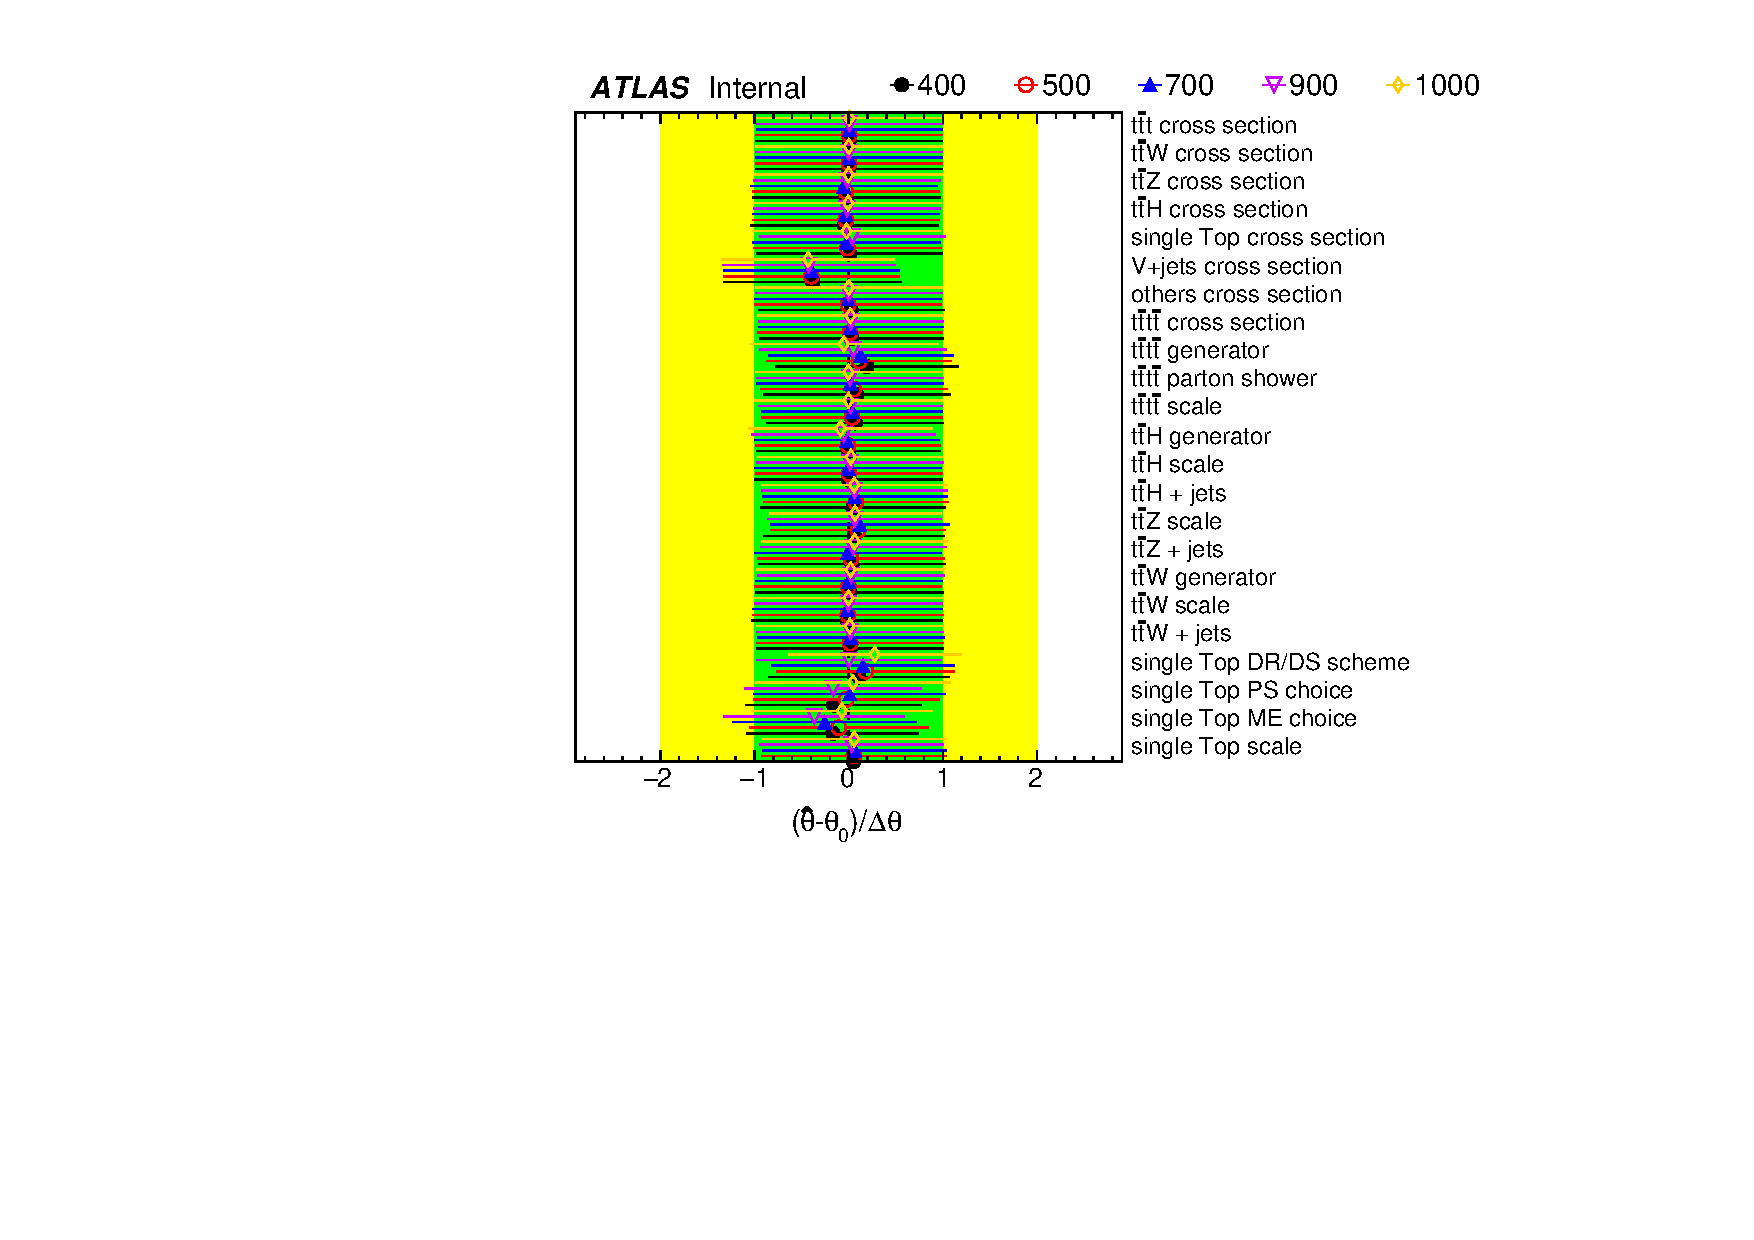
\includegraphics[width=\linewidth]{figures/fits/comparisons/massPoints/GNN/1L/data_unblindedSplusB/NuisPar_comp_Other.pdf}
    \subcaption{1L}
    \label{fig:unblinded_data_SplusB_NP_1L_other}
  \end{subfigure}
  \begin{subfigure}[t]{0.32\textwidth}
    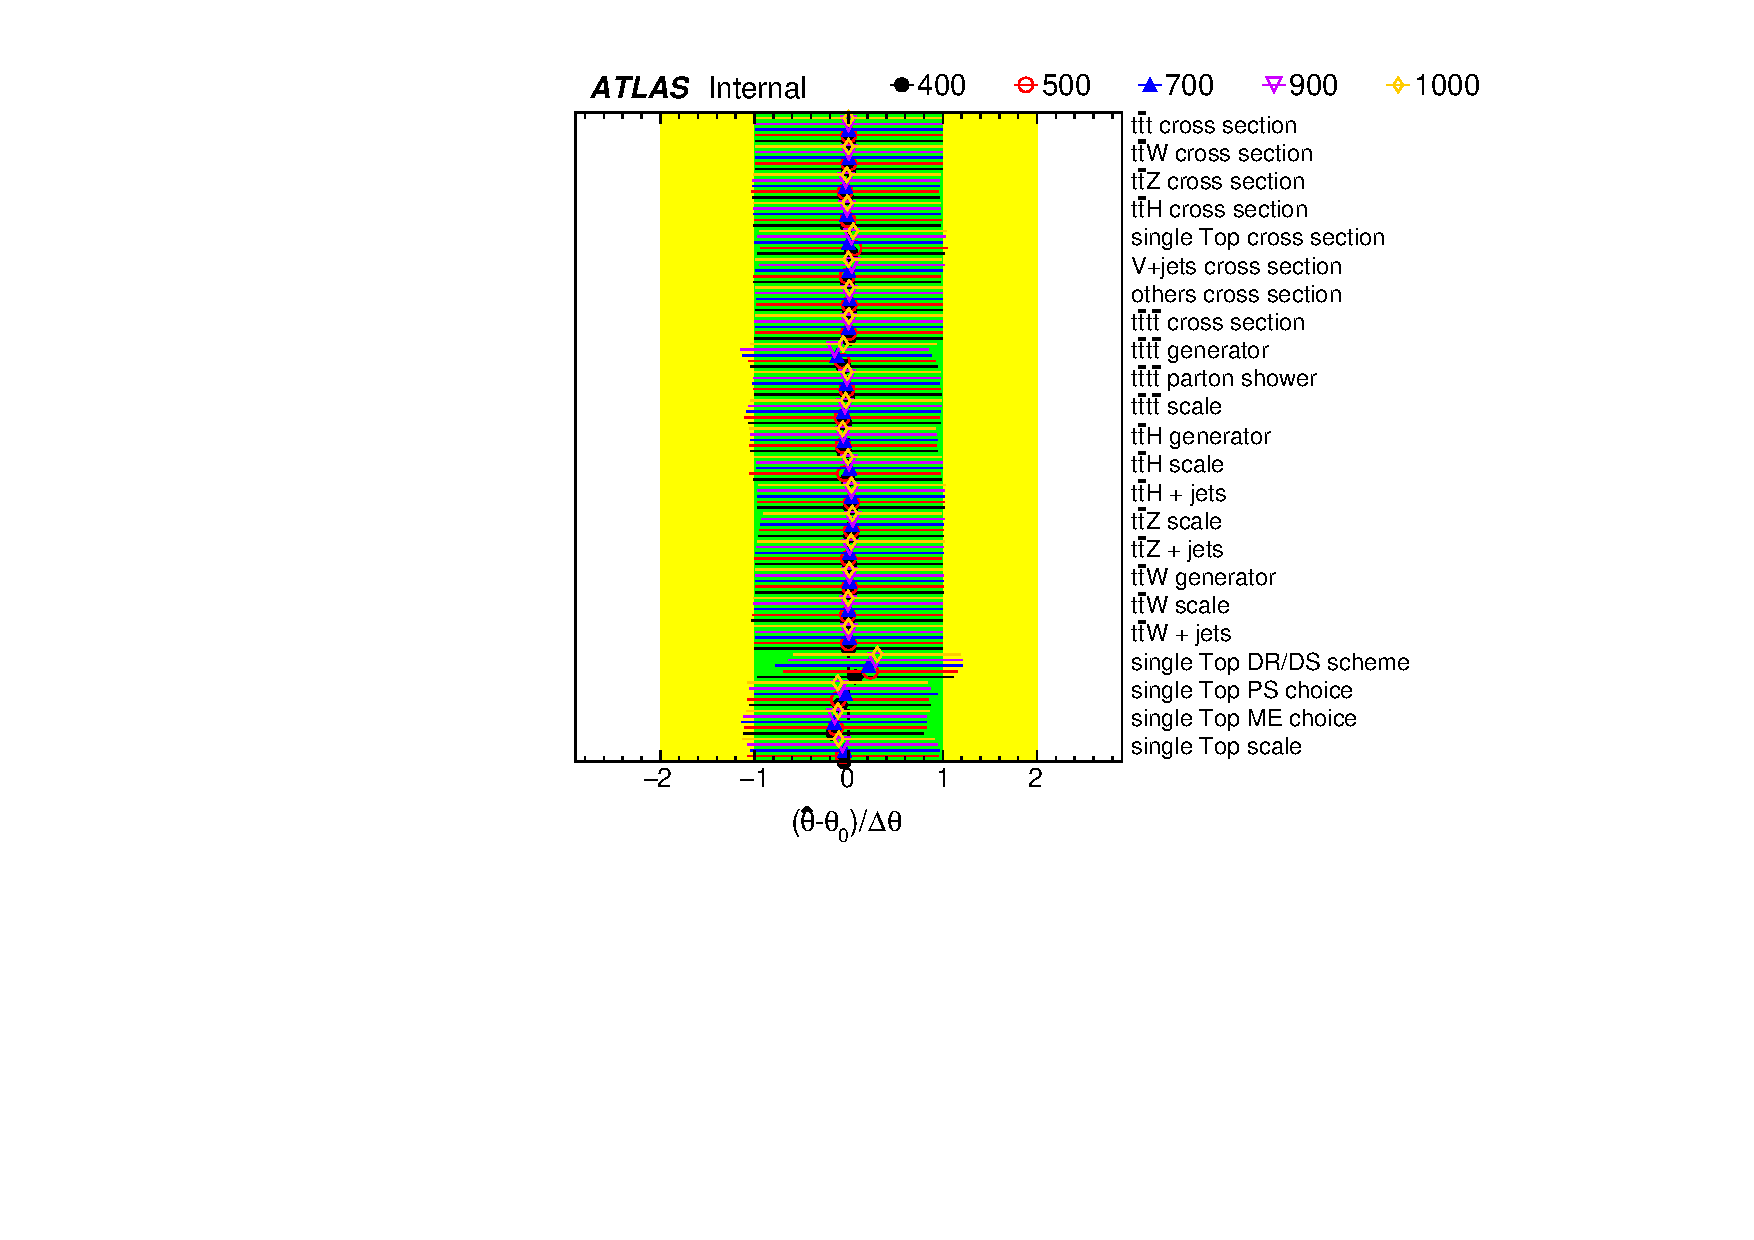
\includegraphics[width=\linewidth]{figures/fits/comparisons/massPoints/GNN/2L/data_unblindedSplusB/NuisPar_comp_Other.pdf}
    \subcaption{2L}
    \label{fig:unblinded_data_SplusB_NP_2L_other}
  \end{subfigure}
  \begin{subfigure}[t]{0.32\textwidth}
    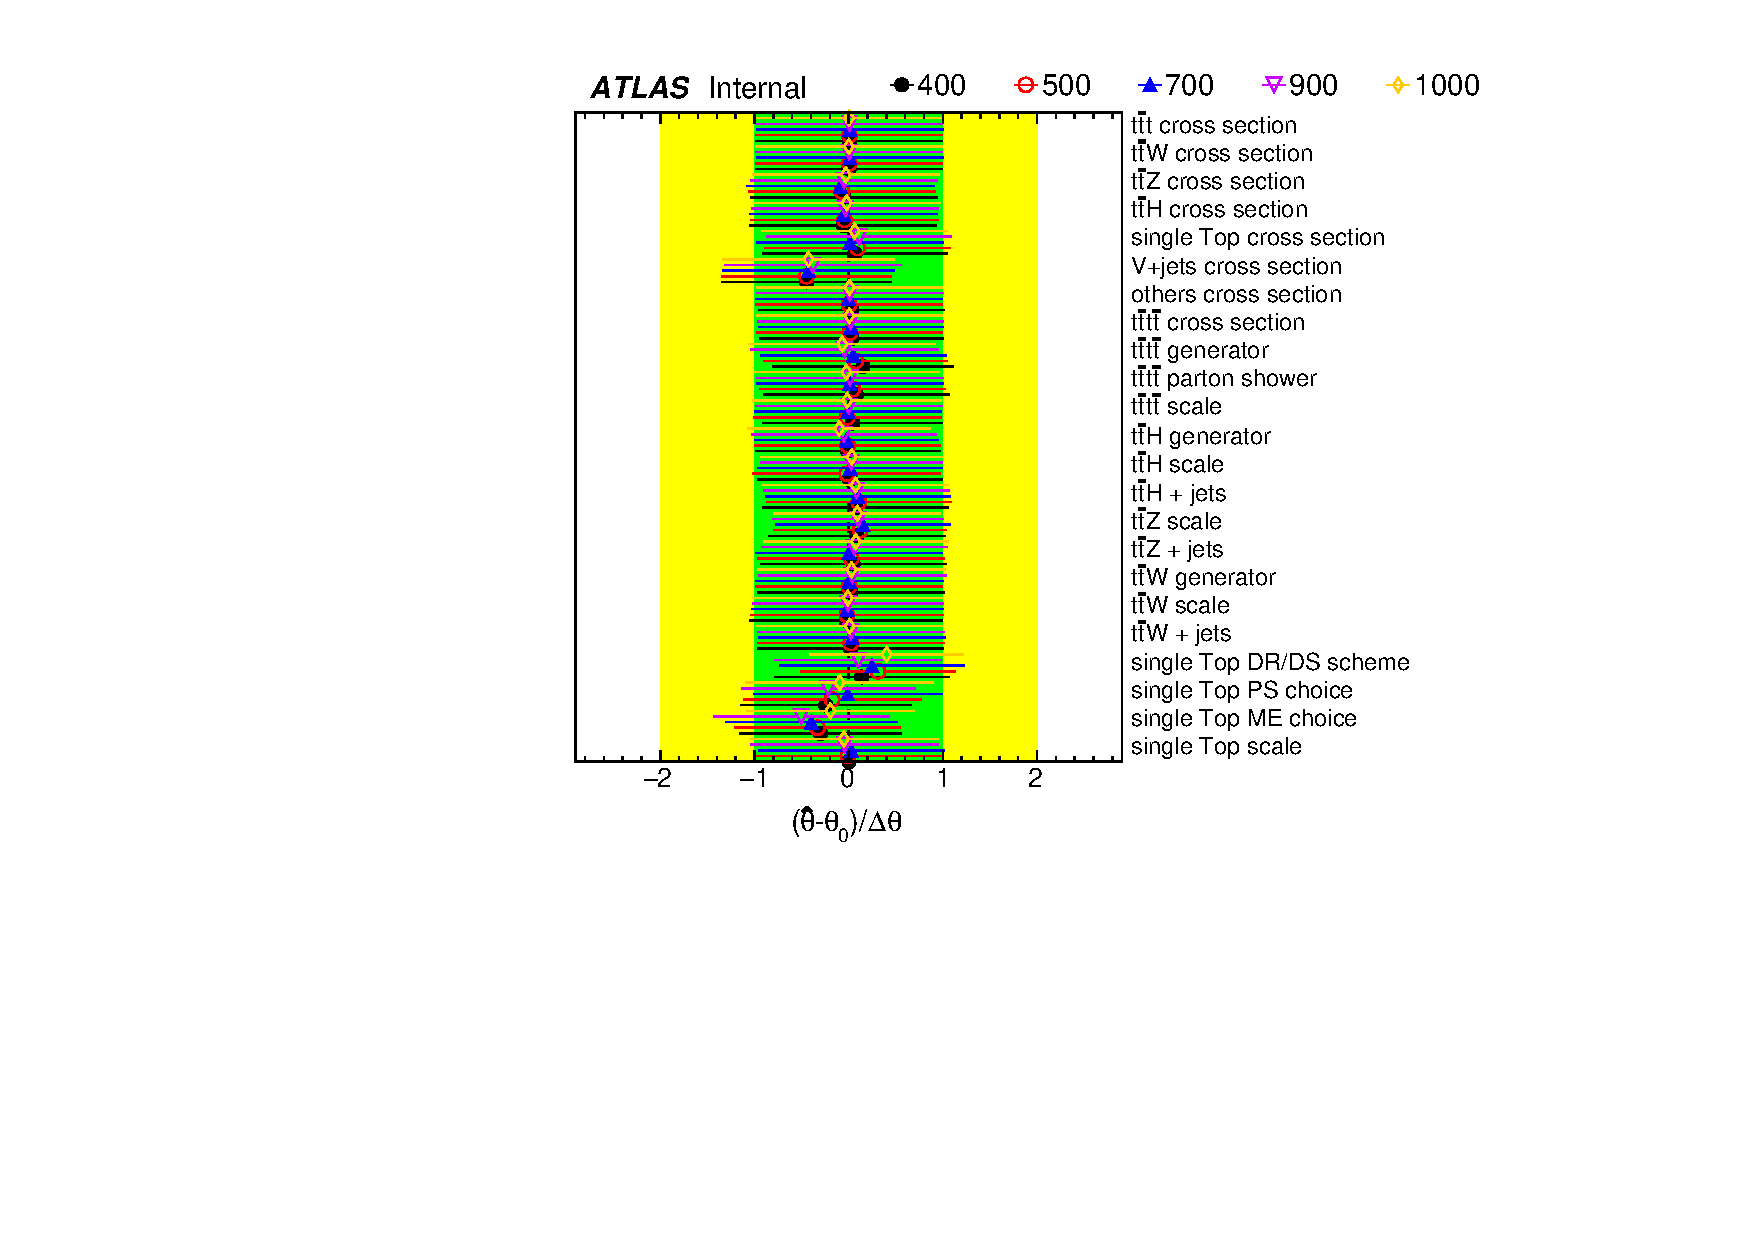
\includegraphics[width=\linewidth]{figures/fits/comparisons/massPoints/GNN/all/data_unblindedSplusB/NuisPar_comp_Other.pdf}
    \subcaption{1L+2L}
    \label{fig:unblinded_data_SplusB_NP_all_other}
  \end{subfigure}
  \caption{Fitted pulls and constraints for the nuisance parameters corresponding to the non-\ttbar-background systematic uncertainties for the signal+background unblinded Data fit for three types of fits: using only 1L regions, using only 2L regions, and using all regions. Comparison is done for five mass points.}
\label{fig:unblinded_data_SplusB_NP_mass_other}
\end{figure}

\begin{figure}[htbp!]
        \centering
        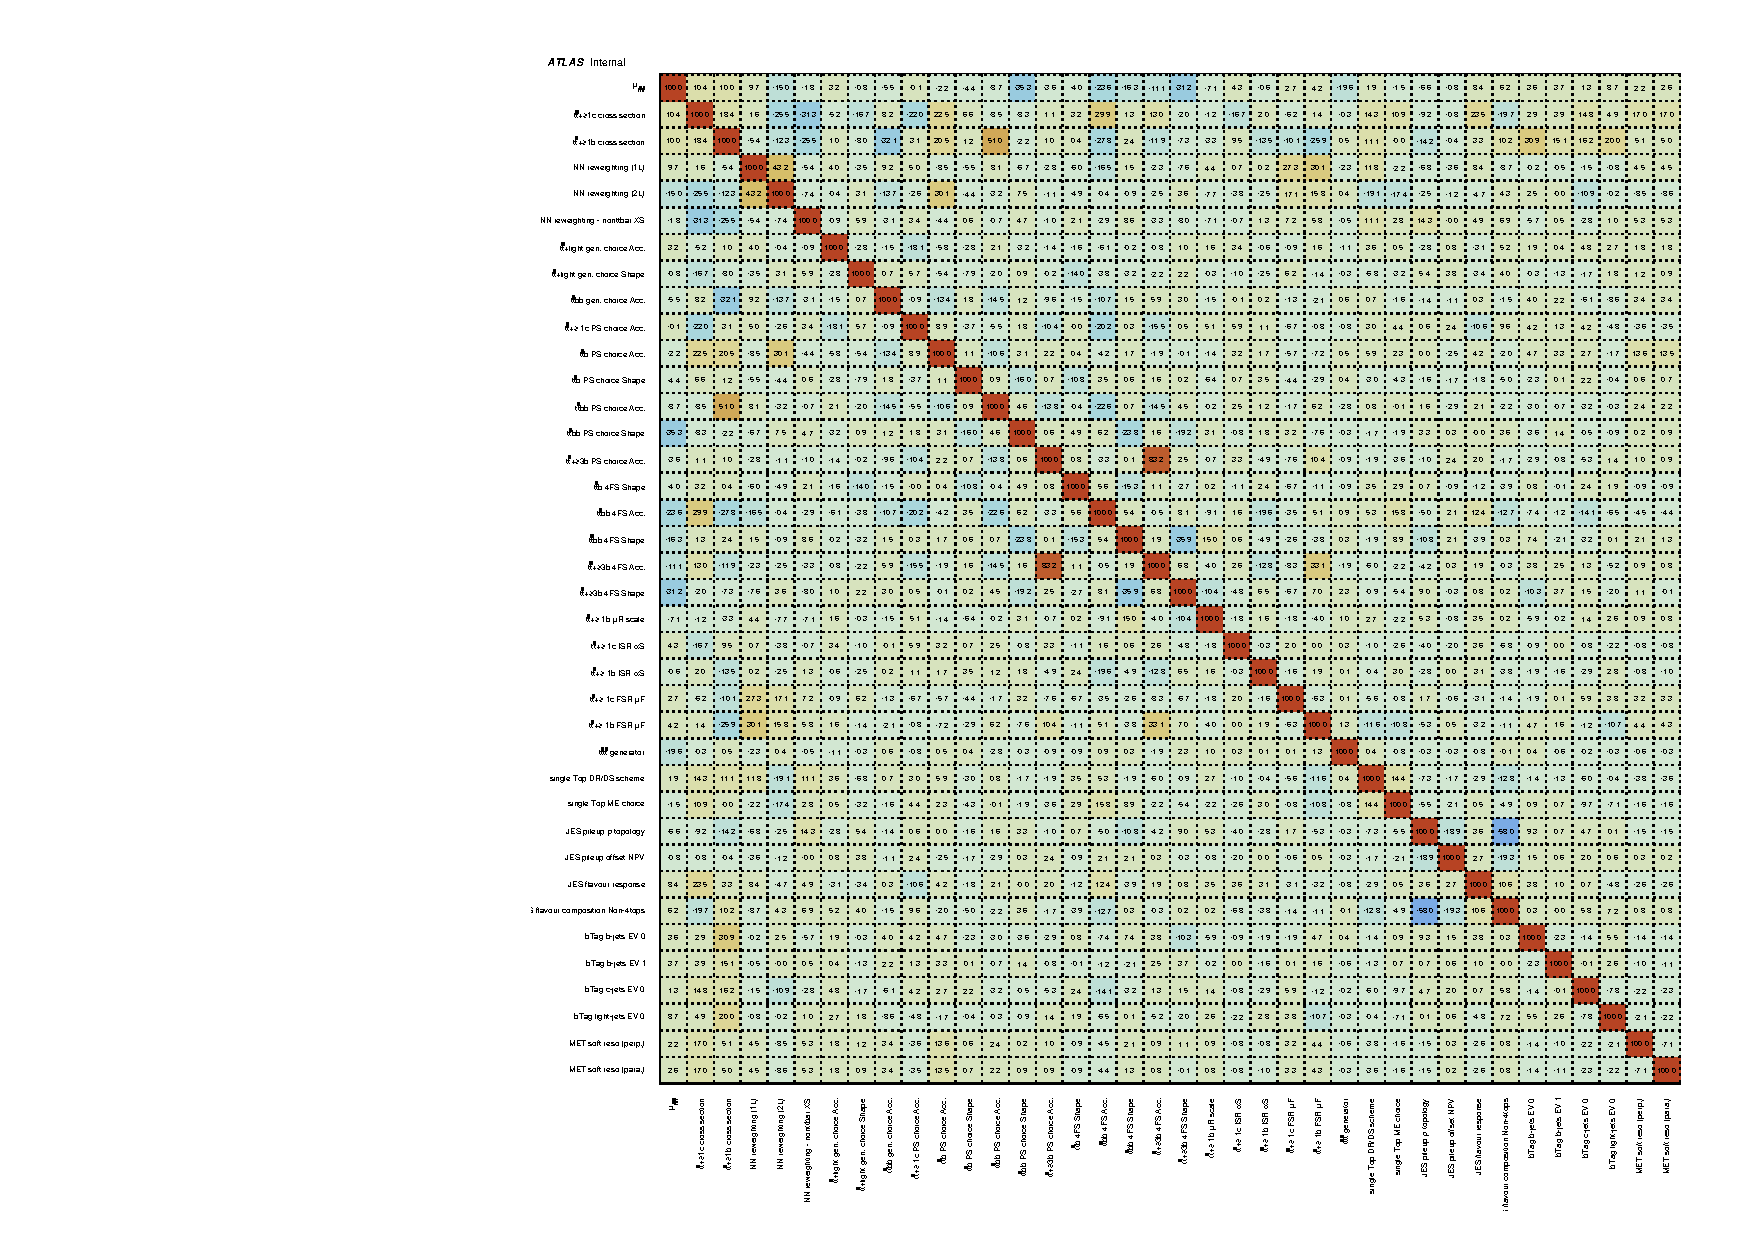
\includegraphics[width=\linewidth]{figures/fits/GNN/400/all/data_unblindedSplusB/CorrMatrix.pdf}
        \caption{\label{fig:unblinded_data_SplusB_corr_mH400_Data_all}Correlation matrix for the signal+background unblinded data fit for mH = 400 GeV}
\end{figure}



\begin{figure}[htbp!]
  \centering
  \begin{subfigure}[t]{0.24\textwidth}
    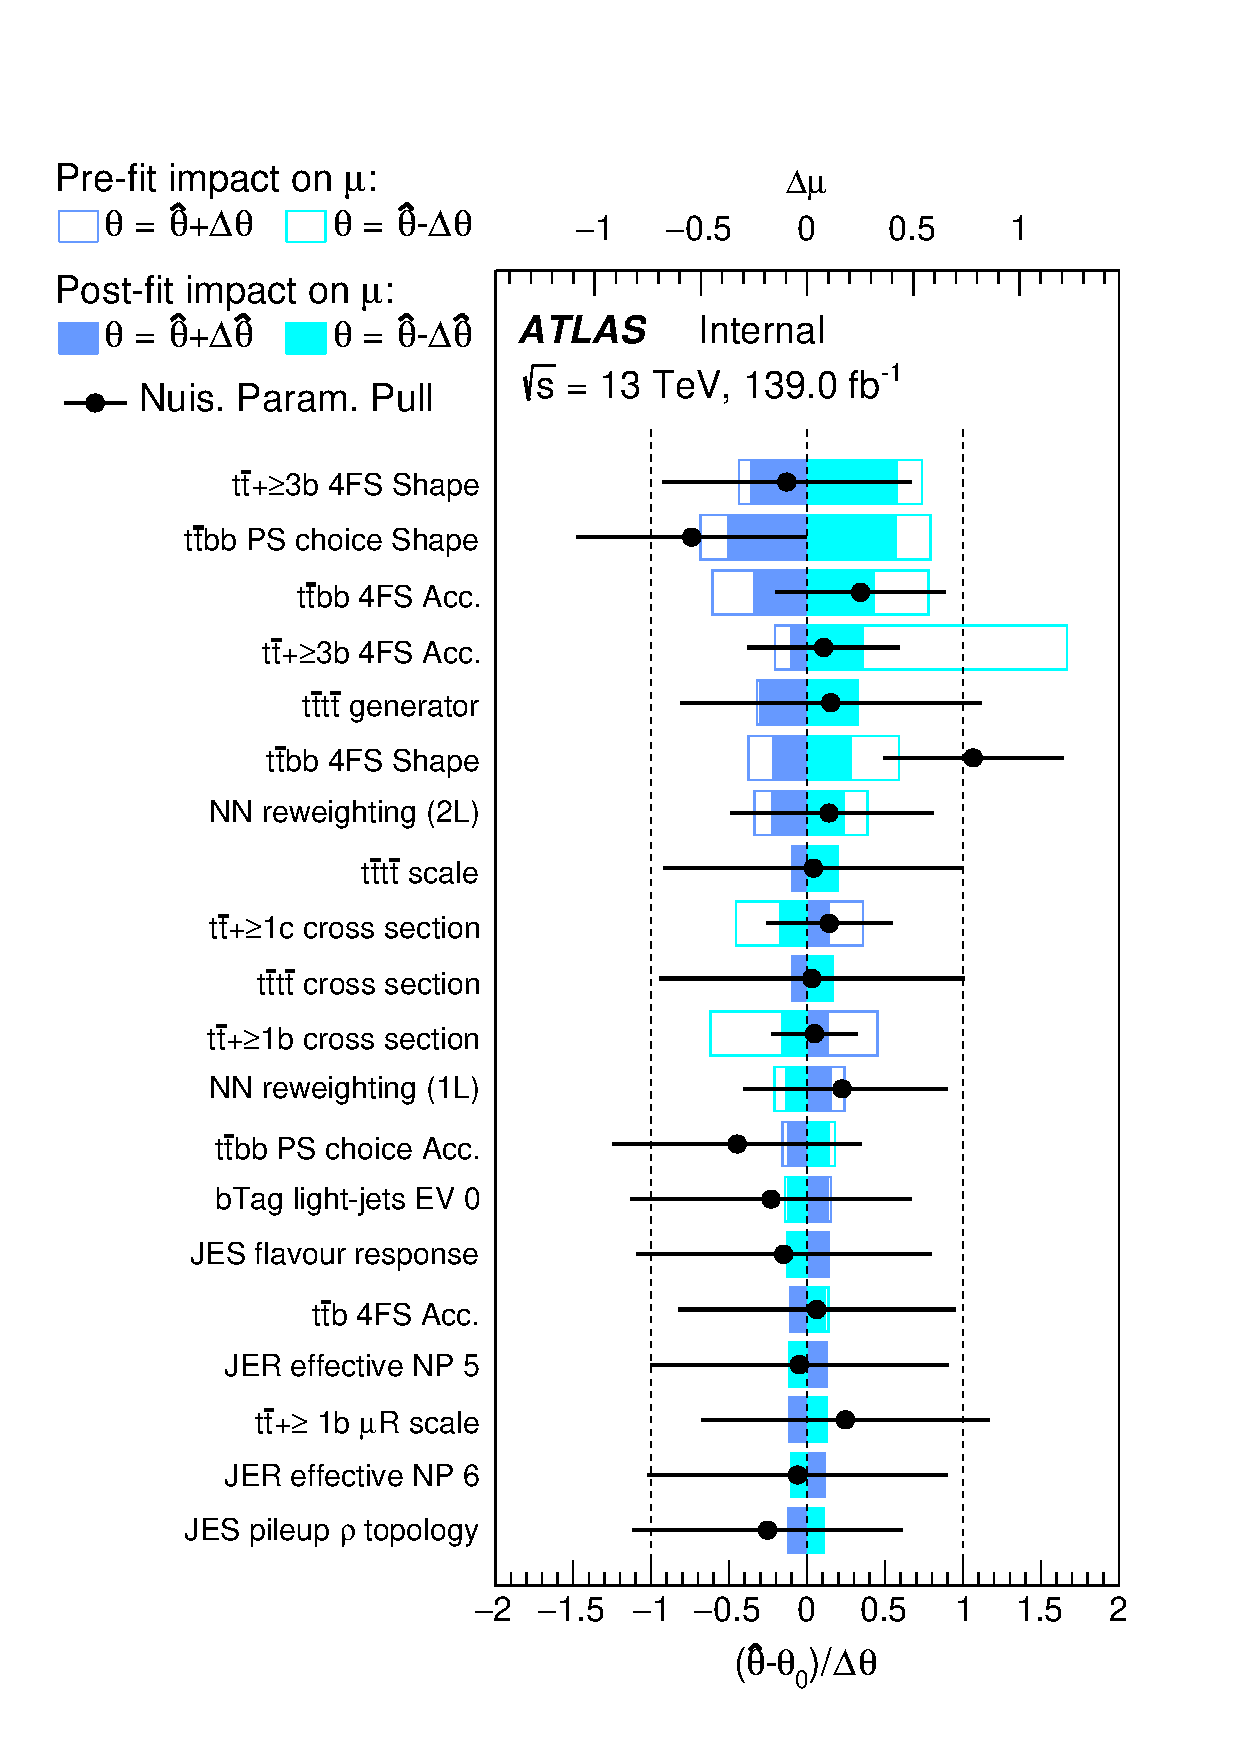
\includegraphics[width=1 \textwidth]{figures/fits/GNN/400/all/data_unblindedSplusB/Ranking_mu_tttt.pdf}
    \caption{\label{fig:Ranking_data_SplusB_400}400\gev }
  \end{subfigure}
  \begin{subfigure}[t]{0.24\textwidth}
    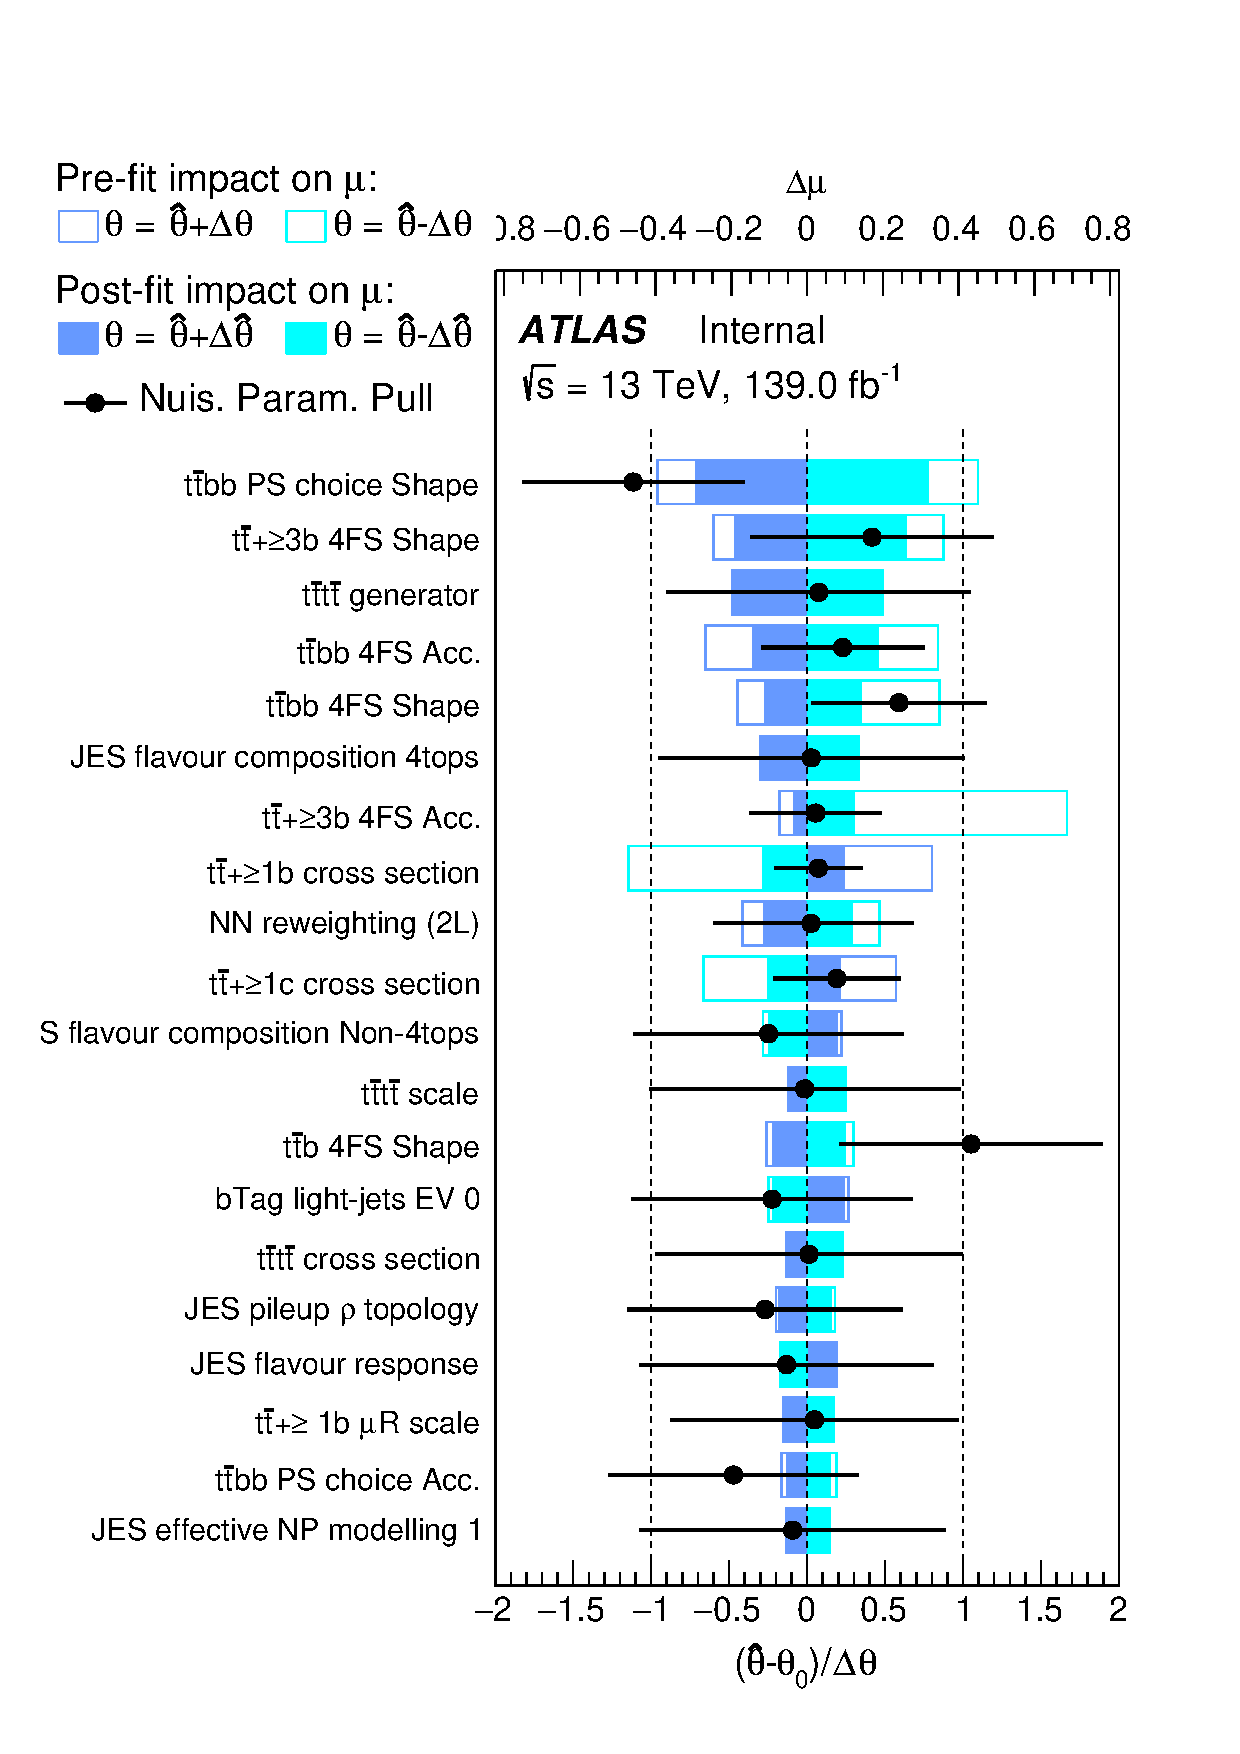
\includegraphics[width=1 \textwidth]{figures/fits/GNN/500/all/data_unblindedSplusB/Ranking_mu_tttt.pdf}
    \caption{\label{fig:Ranking_data_SplusB_500}500\gev }
  \end{subfigure}
  \begin{subfigure}[t]{0.24\textwidth}
    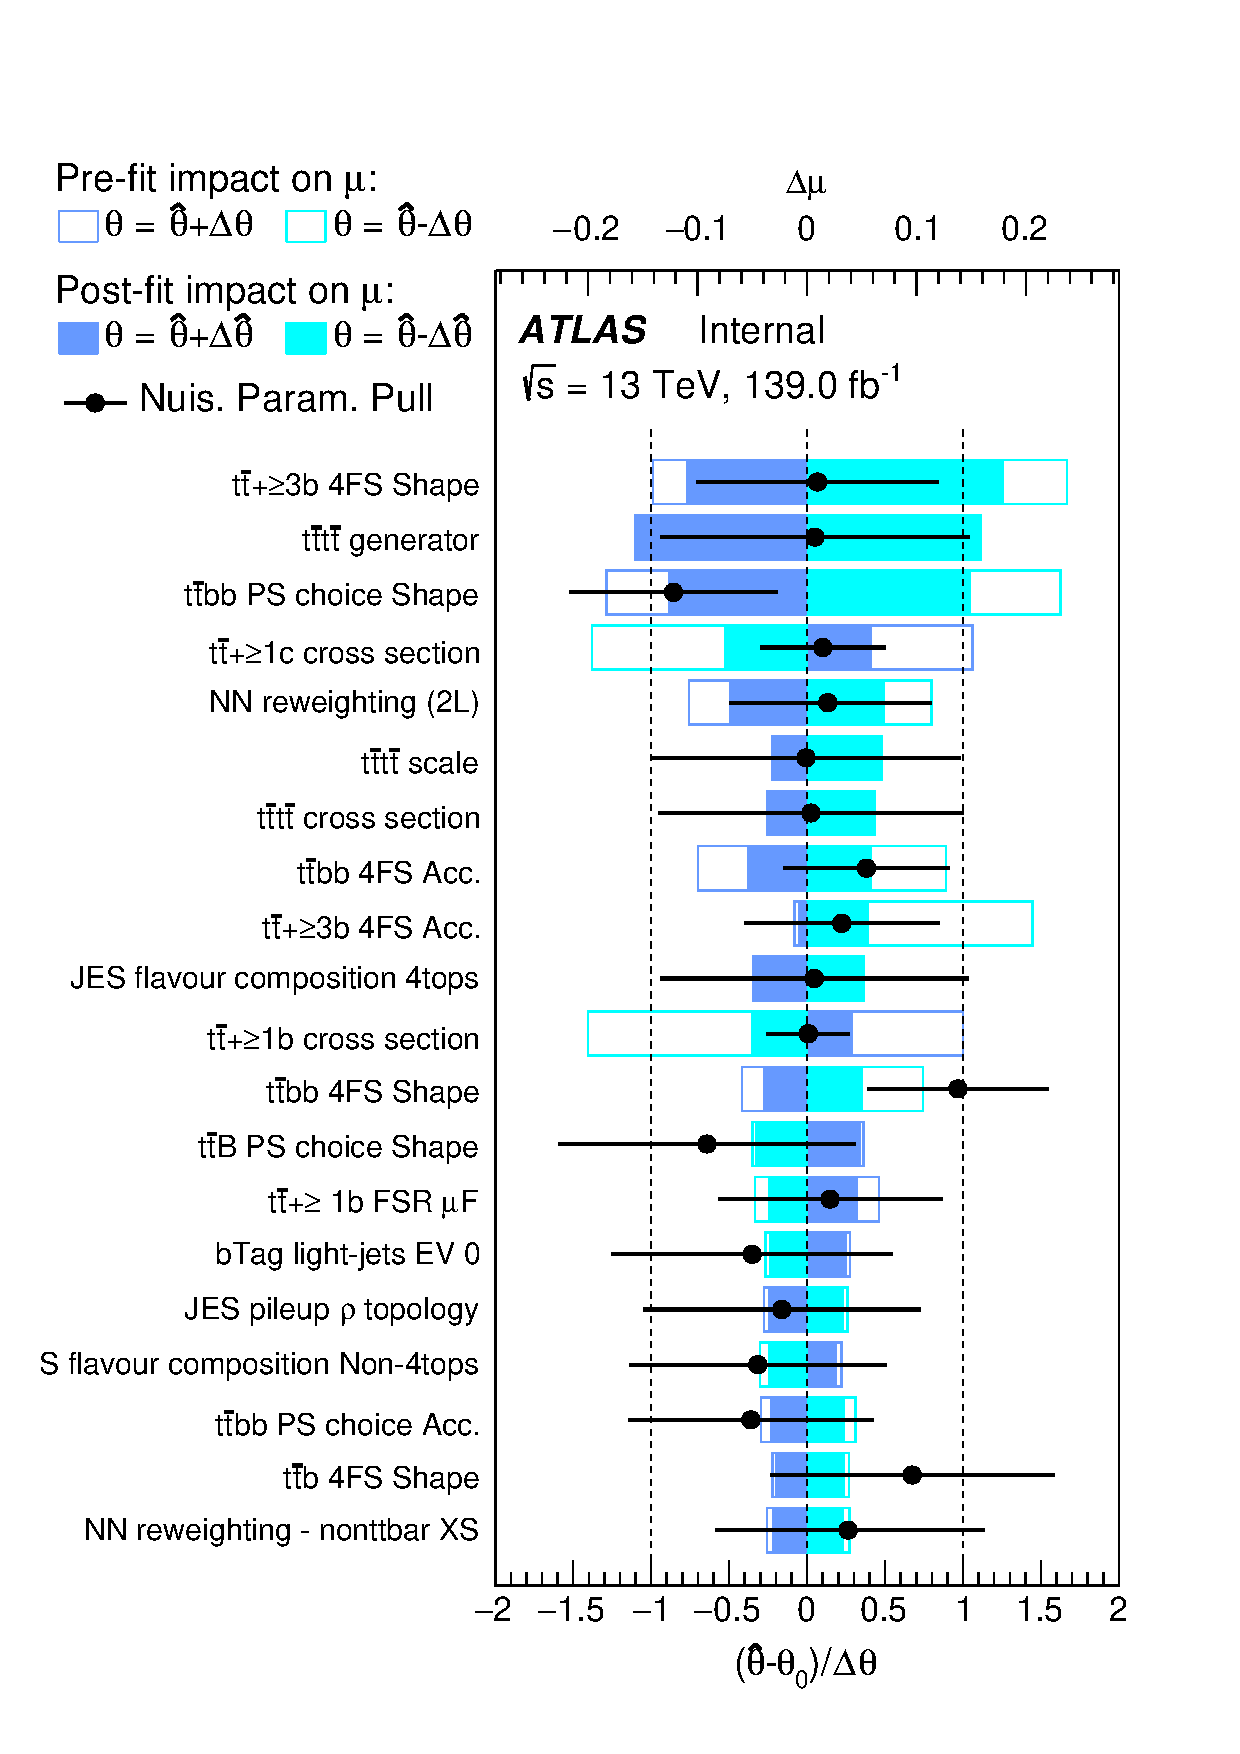
\includegraphics[width=1 \textwidth]{figures/fits/GNN/700/all/data_unblindedSplusB/Ranking_mu_tttt.pdf}
    \caption{\label{fig:Ranking_data_SplusB_700}700\gev }
  \end{subfigure}
  \begin{subfigure}[t]{0.24\textwidth}
    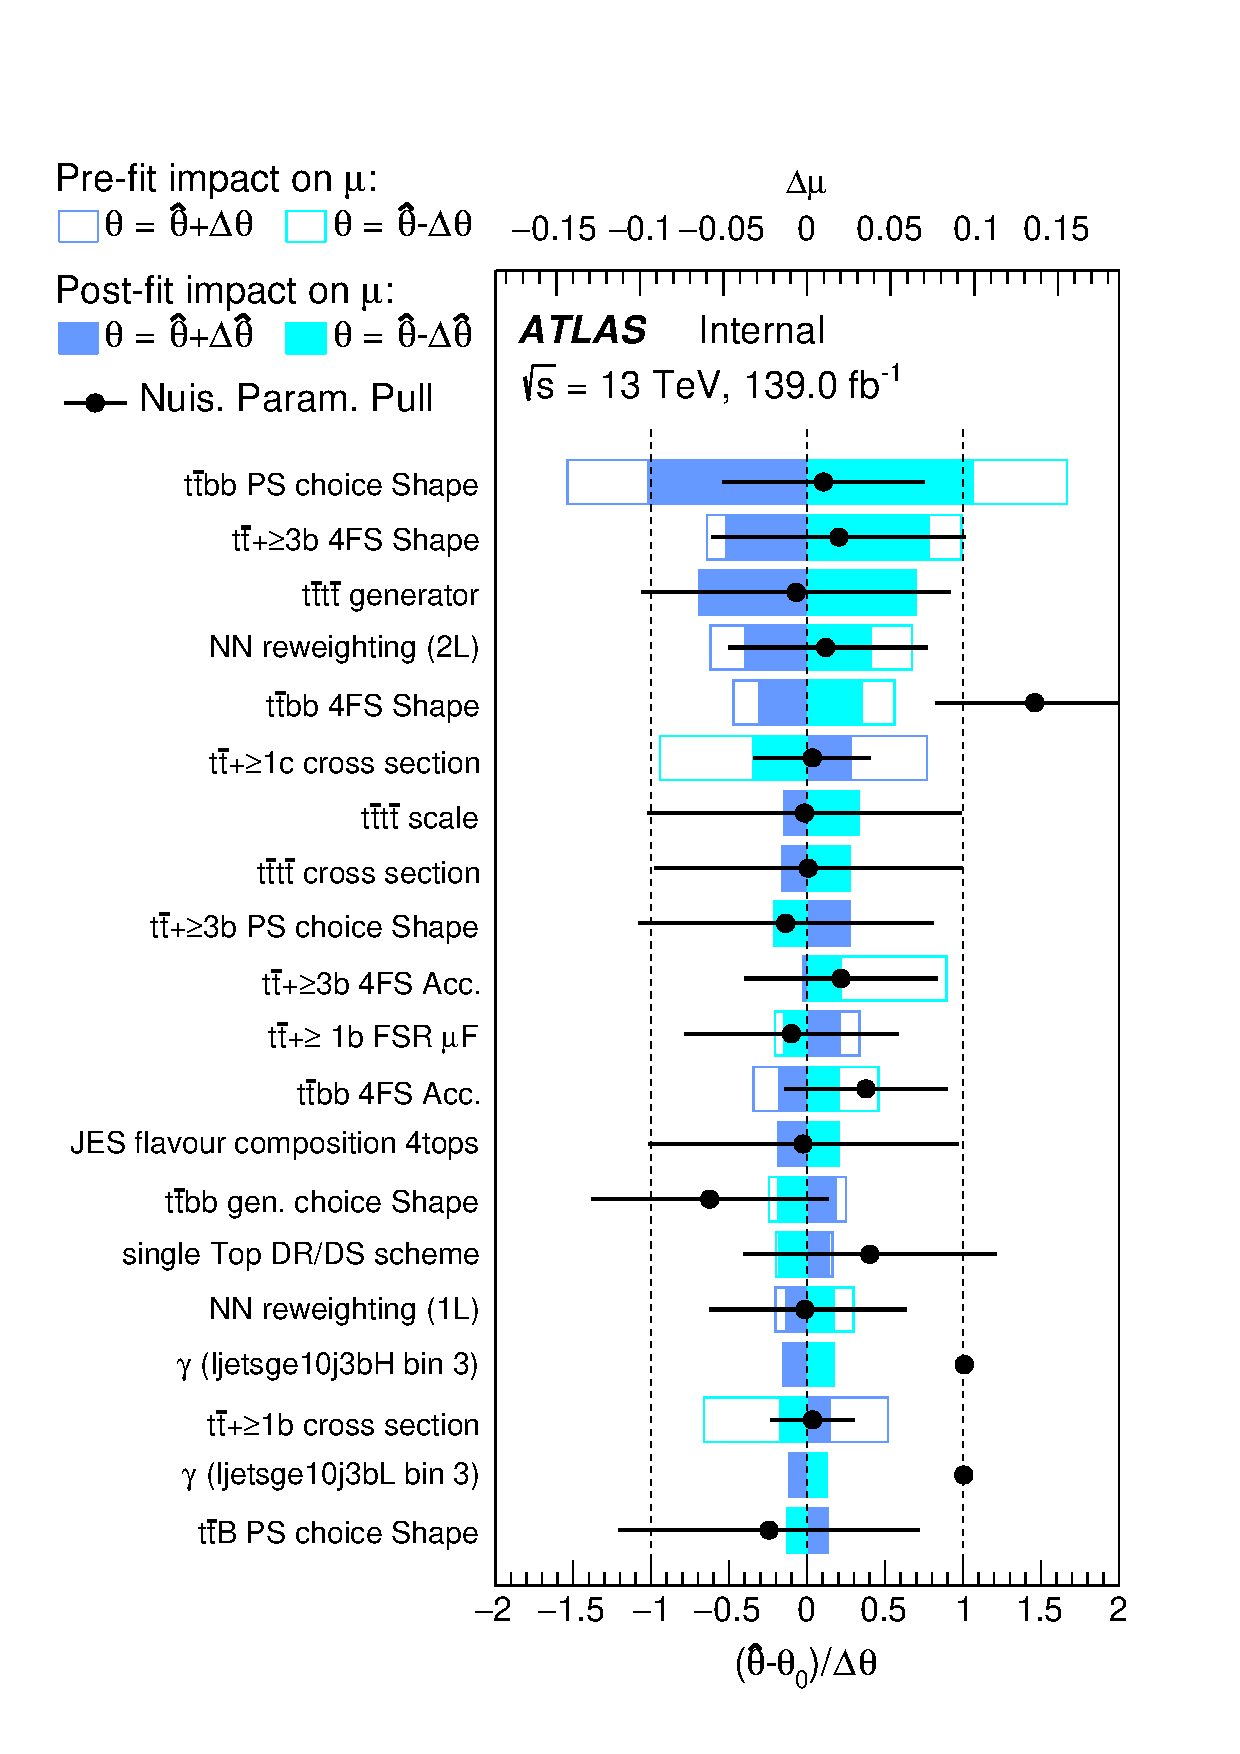
\includegraphics[width=1 \textwidth]{figures/fits/GNN/1000/all/data_unblindedSplusB/Ranking_mu_tttt.pdf}
    \caption{\label{fig:Ranking_data_SplusB_1000}1000\gev }
  \end{subfigure}
  \caption{\label{fig:Ranking_mH700_Asimov}Fitted pulls and constraints for the nuisance parameters ranked by their impact for four mass points types of signal+background unblinded data fit.}
\end{figure}



\subsubsection{2HDM interpretation}
\label{sec:limits_data}
The expected and observed limits on cross section of BSM $\fourtops$ using all regions (1L+2L) are shown in Figure \ref{fig:data_SplusB_limits}. Exclusion limit of $\tan\beta$ as a function of $m_{H/A}$ is shown in Figure \ref{fig:1LOS_2Dplots}. The combination with the previous search using SSML regions is shown in Section \ref{sec:combination}.

\begin{figure}[htbp!]
  \centering
  \begin{subfigure}[t]{0.49\textwidth}
    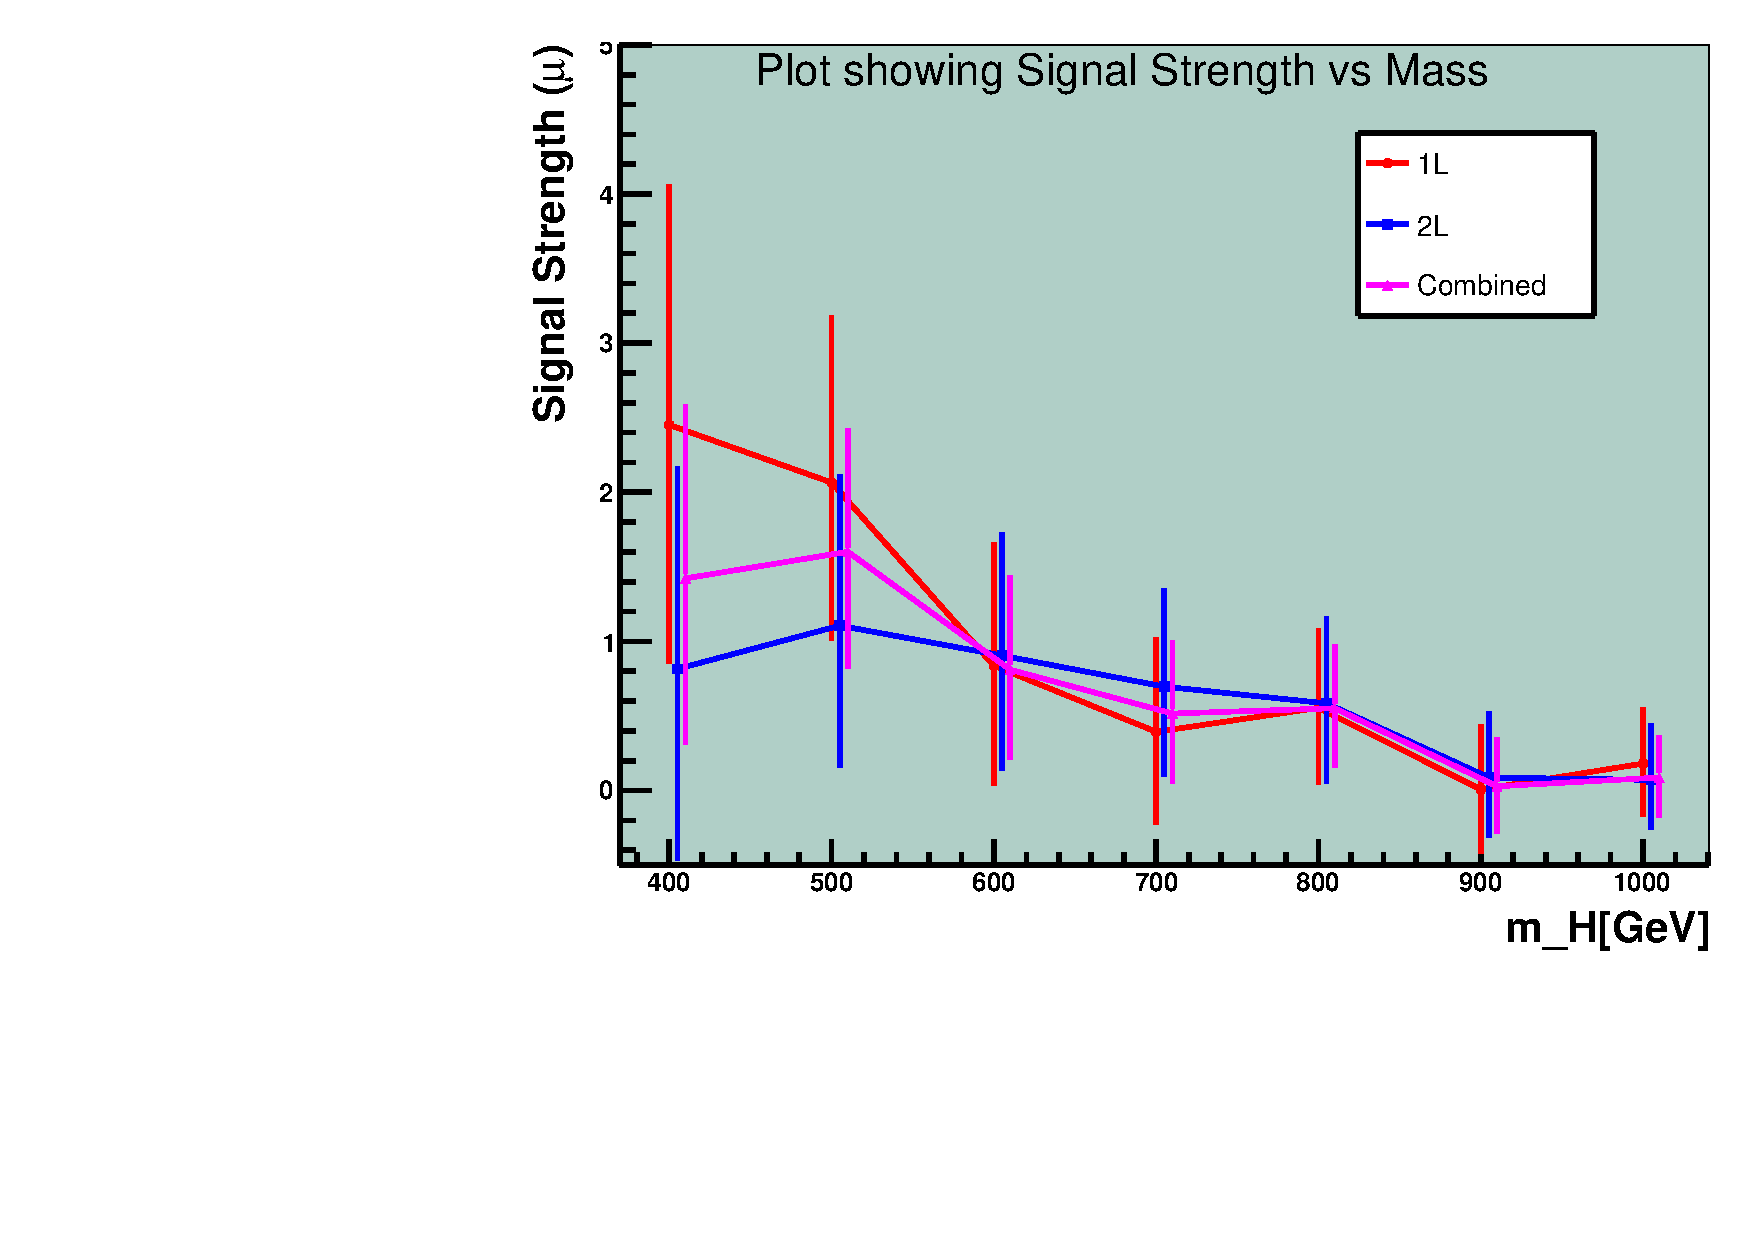
\includegraphics[width=1 \textwidth]{figures/fits/signalStrengthVsMass.pdf}
    \caption{\label{fig:data_SplusB_signal_strength}Signal strength}
  \end{subfigure}
  \begin{subfigure}[t]{0.49\textwidth}
    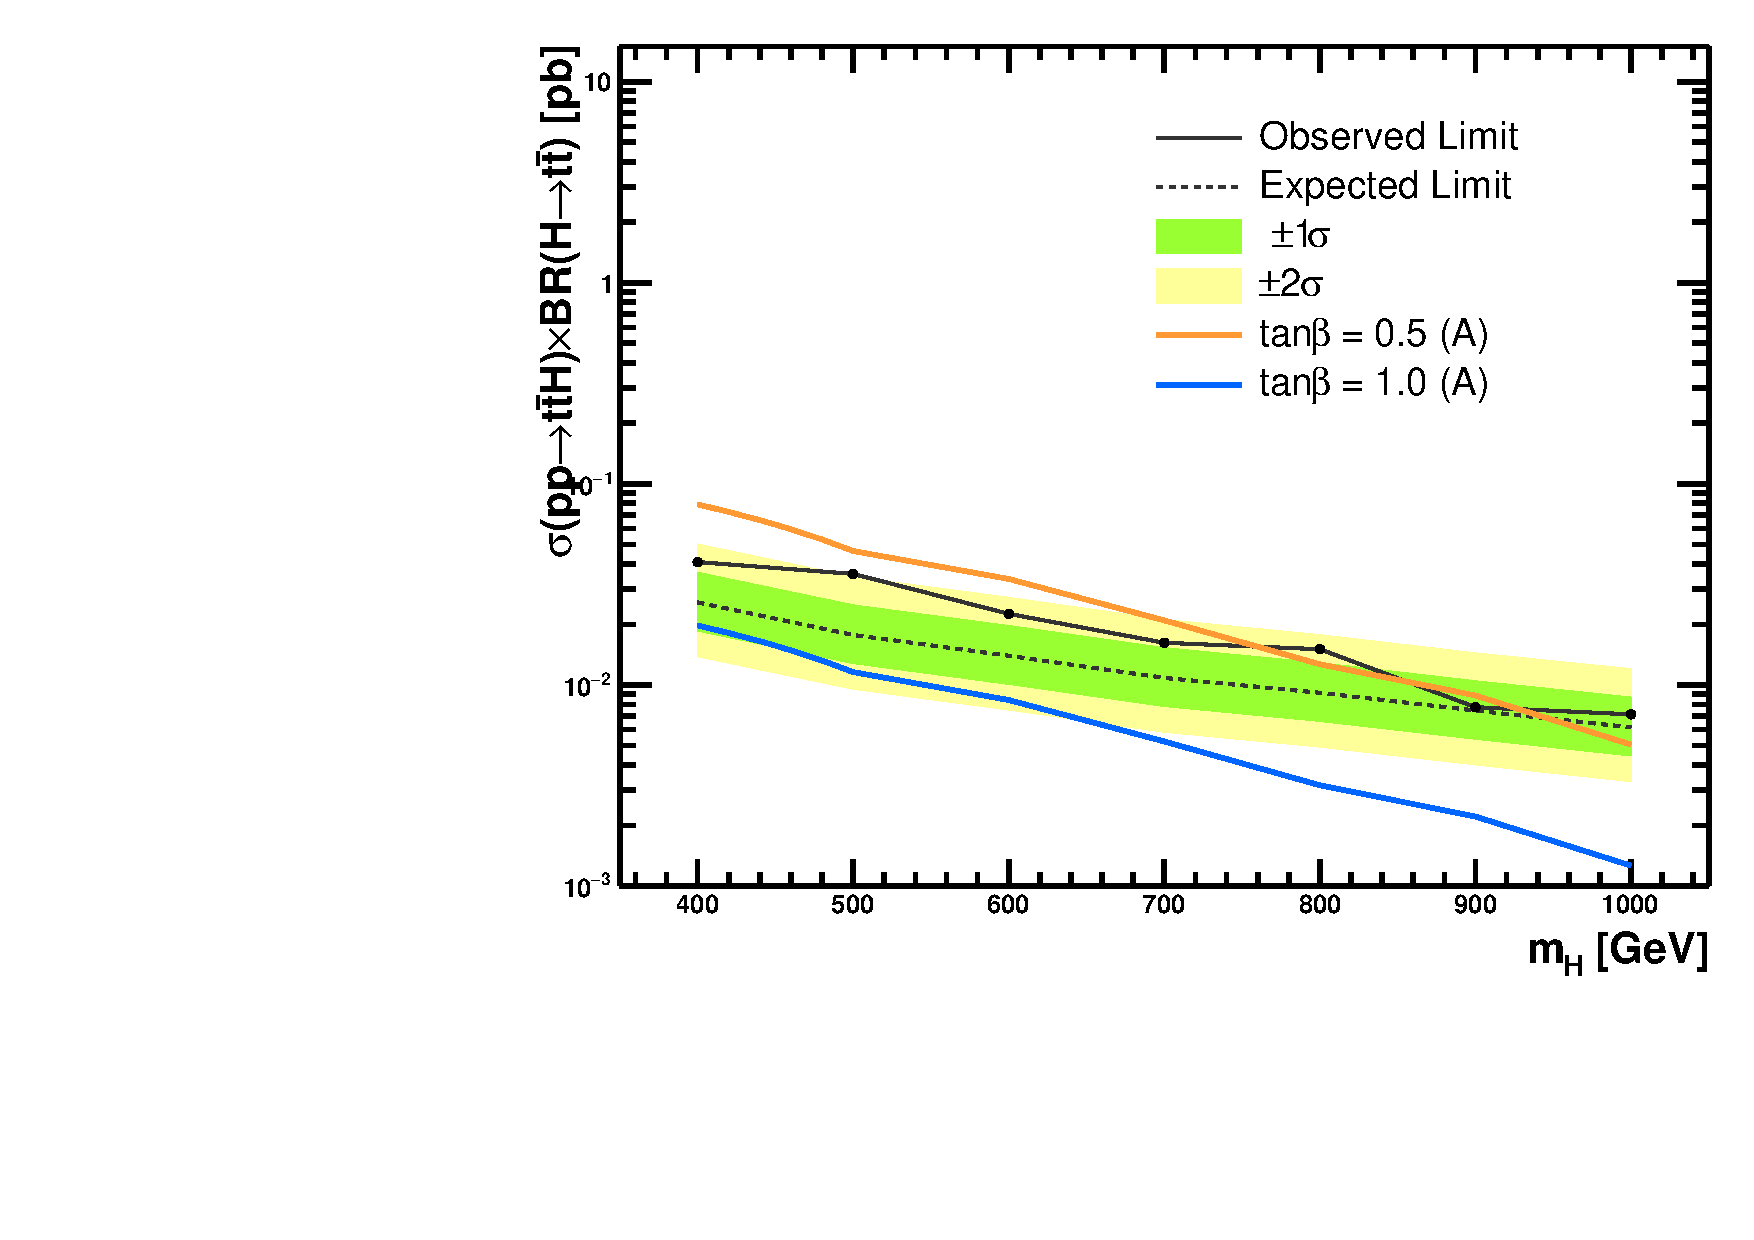
\includegraphics[width=1 \textwidth]{figures/fits/limits_Obs.pdf}
    \caption{\label{fig:data_SplusB_limits}Expected and observed limits}
  \end{subfigure}
  \caption{\label{fig:data_SplusB}Comparison of the expected and observed 95\% CL upper limits on the cross section times branching fraction to \ttbar for the production of a heavy higgs boson~\ttHA~as a function of $m_{H/A}$ for unblinded data fit. Theoretical predictions for two values of $\tan\beta$ are shown.}
\end{figure}

\begin{figure}[htbp!]
  \centering
  \begin{subfigure}[t]{0.49\textwidth}
    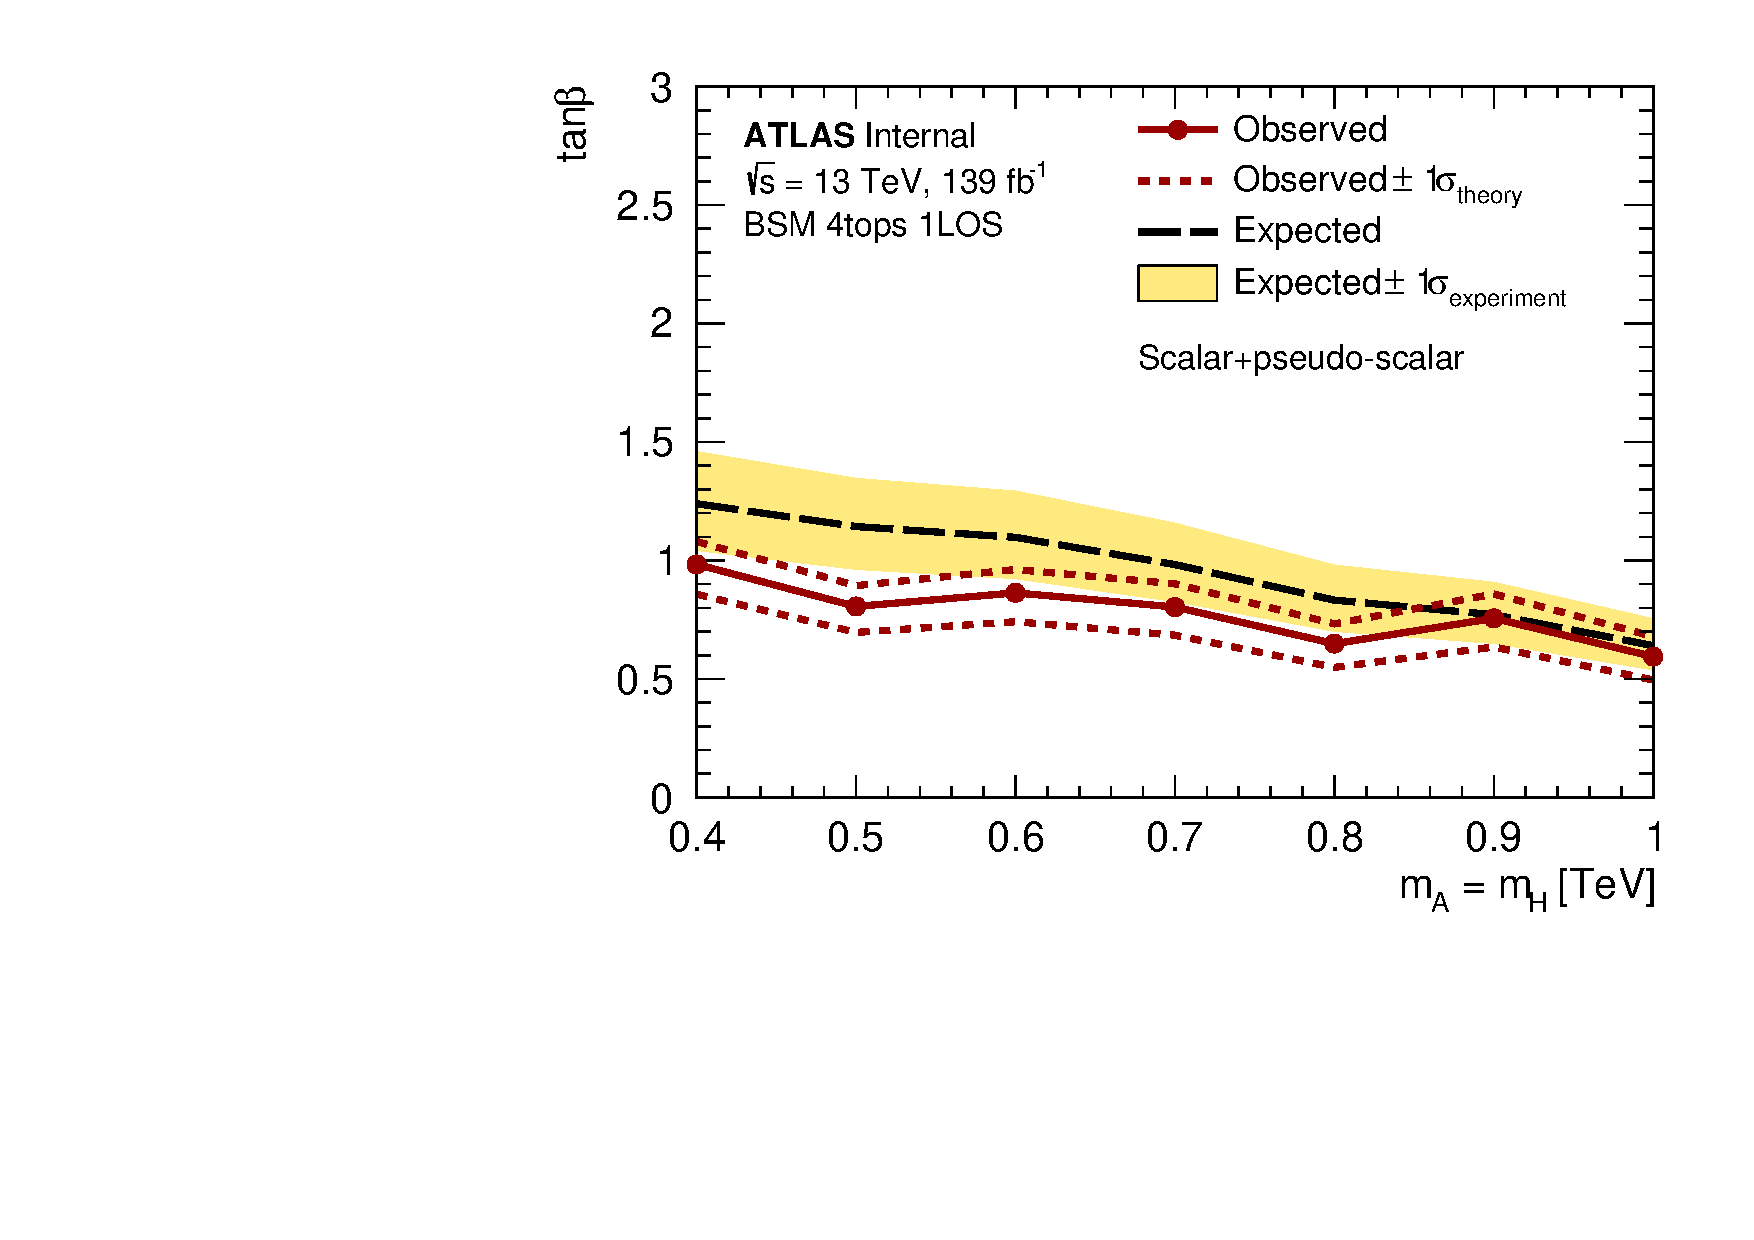
\includegraphics[width=1 \textwidth]{figures/fits/2D_plots/Data_12fb_All_1LOS.pdf}
    \caption{}
  \end{subfigure}
  \\
  \begin{subfigure}[t]{0.49\textwidth}
    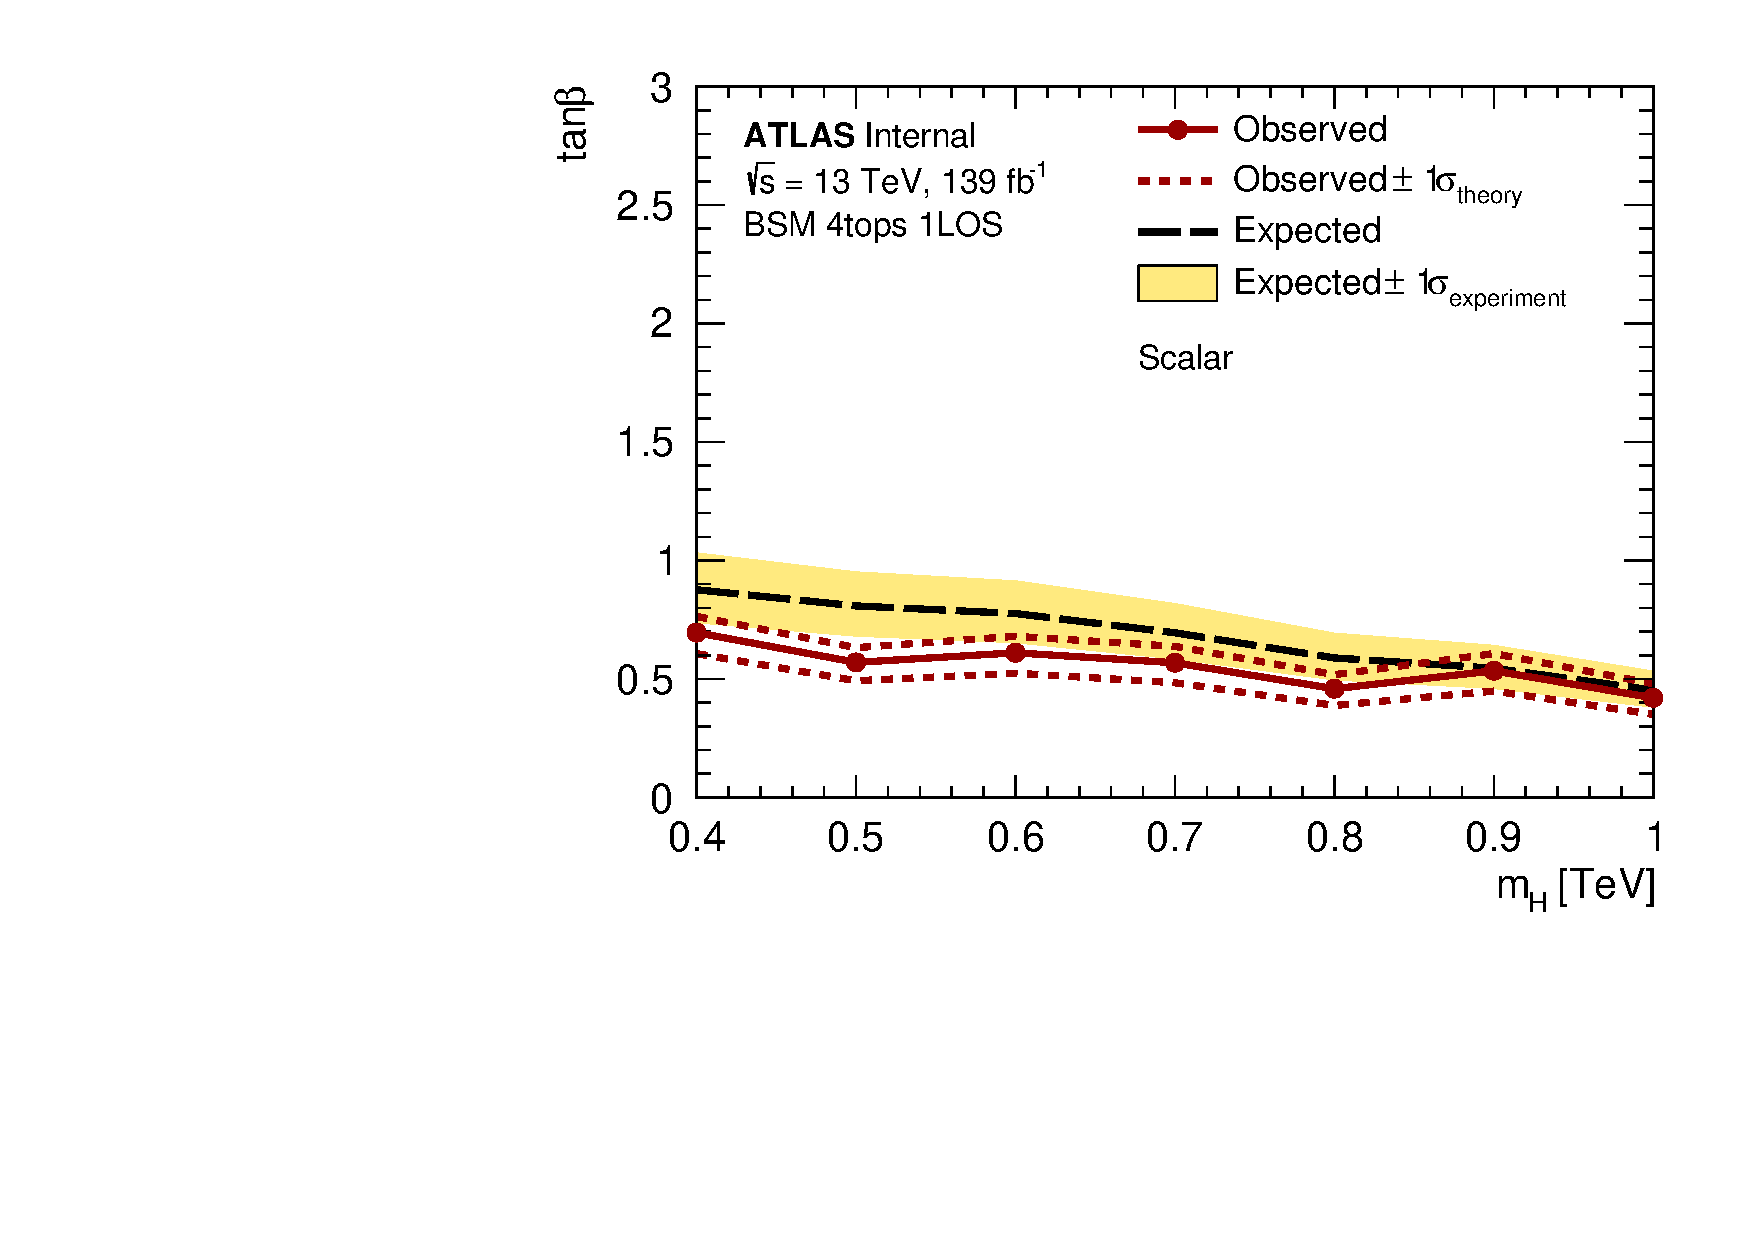
\includegraphics[width=1 \textwidth]{figures/fits/2D_plots/Data_12fb_ttH_1LOS.pdf}
    \caption{}
  \end{subfigure}
  \begin{subfigure}[t]{0.49\textwidth}
    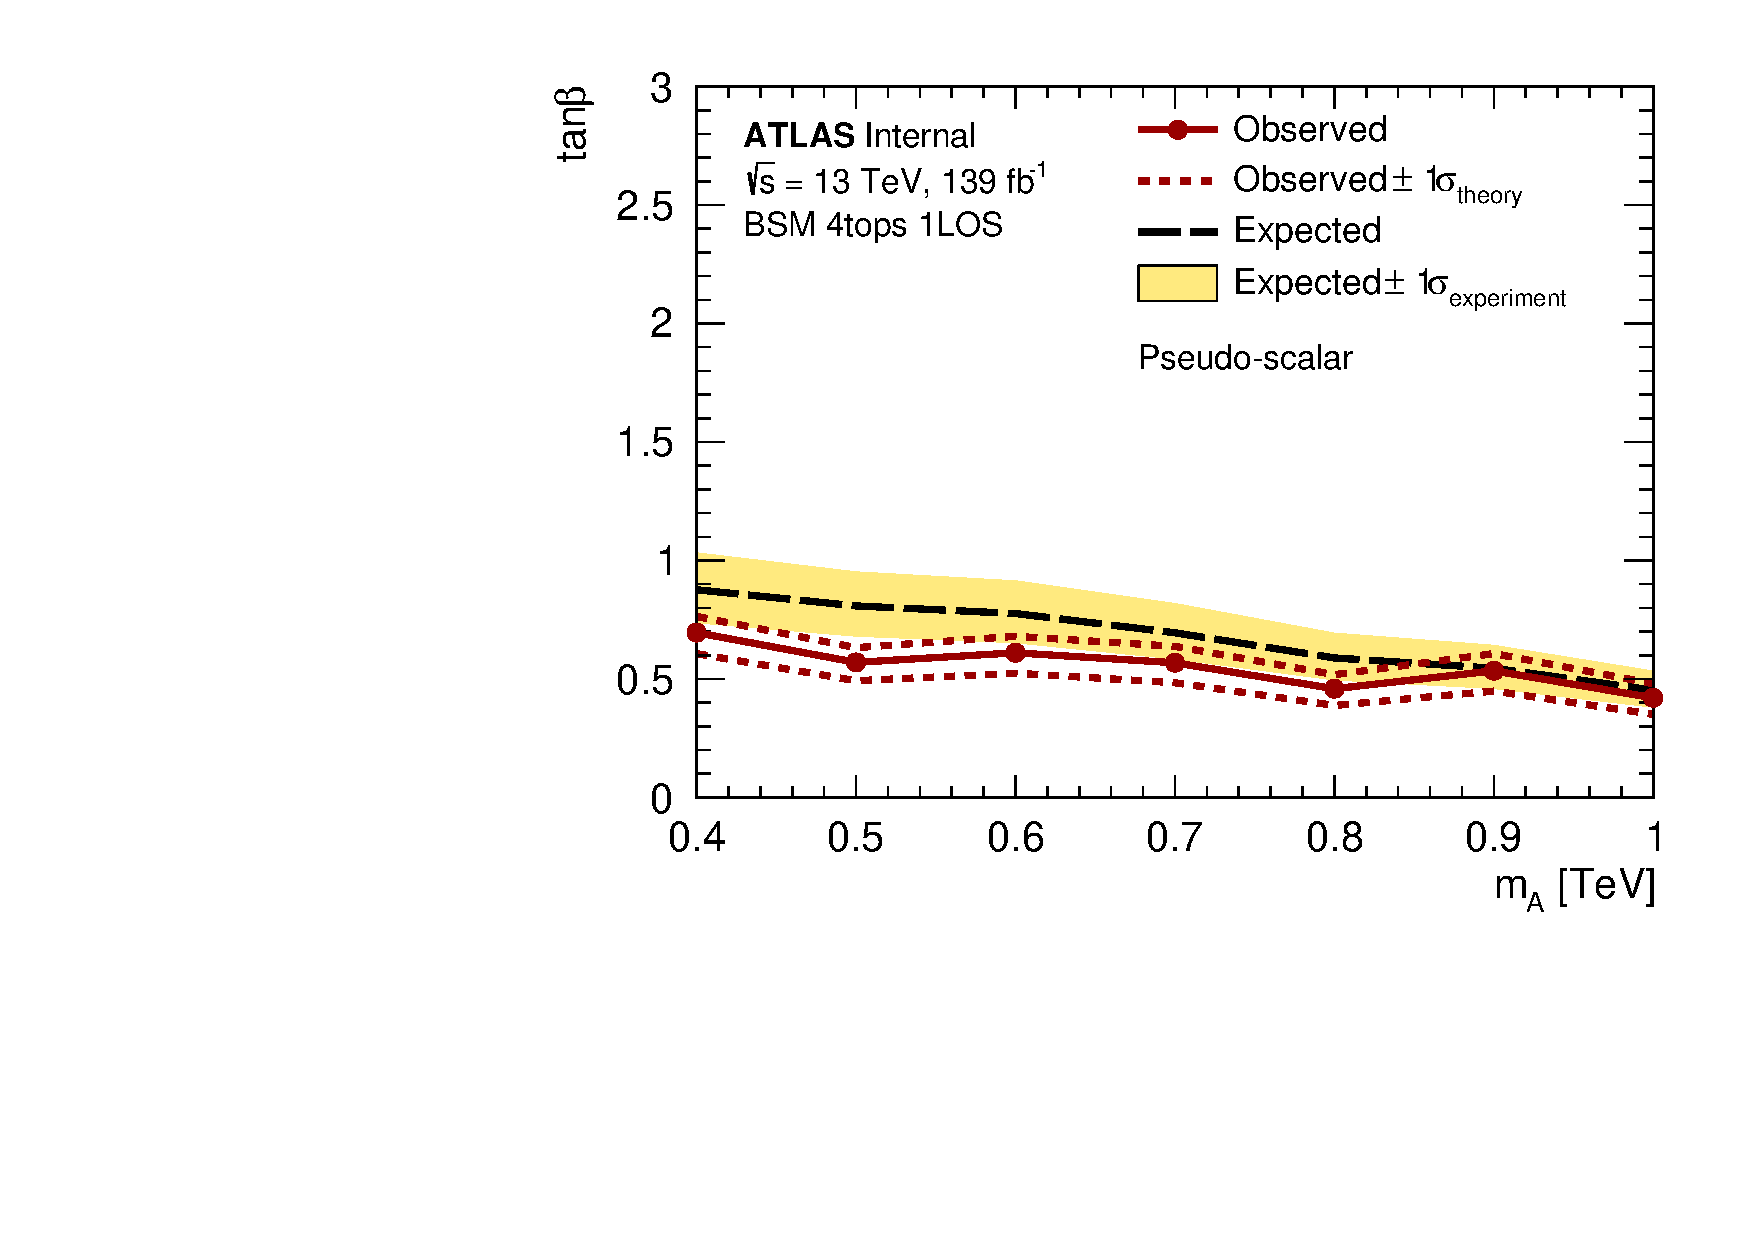
\includegraphics[width=1 \textwidth]{figures/fits/2D_plots/Data_12fb_ttA_1LOS.pdf}
    \caption{}
  \end{subfigure}
  \caption{\label{fig:1LOS_2Dplots}Observed and expected exclusion regions at 95$\%$ CL in the $\tan\beta$ versus mass plane assuming that both, a heavy scalar $H$ and pseudo-scalar $A$, contribute to the $t\bar{t}t\bar{t}$ final state and have the same mass $m_{H}=m_{A}$ (a), or assuming that only the scalar $H$ (b) or the pseudo-scalar $A$ contributes (c). The yellow band shows the $\pm1\sigma$ variation on the expected exclusion region. The region below the red solid line is excluded at 95$\%$ CL. The exclusion regions are derived in the context of 2HDM type-II.}
\end{figure}